\documentclass[12pt, block=fill]{beamer}
\usepackage{graphicx}
% \usepackage[sfdefault]{FiraSans}
% \usepackage{FiraMono}
\usepackage[T1]{fontenc}
\usepackage{xcolor}
% \usepackage{mathtools}
\usepackage{txfonts}
\usepackage{amsmath}


\usepackage{hyperref}

\definecolor{burntOrange}{rgb}{.8, .5, .1}
\definecolor{textgray}{rgb}{.8,.8,.8}
\definecolor{berkeleyBlue}{cmyk}{100,71,10,47}
\definecolor{berkeleyYellow}{HTML}{FDB515}

% \setbeamercolor{frametitle}{bg=berkeleyBlue}

\usetheme[
titleformat frame = smallcaps,
subsectionpage = progressbar]
{metropolis}

\metroset{
  block=fill
}

\usepackage{pgfpages}
  \setbeameroption{hide notes} % Only slides
% \setbeameroption{show only notes} % Only notes
%  \setbeameroption{show notes on second screen=right} % Both
  
\setbeamerfont{note page}{size=\footnotesize}

\newcommand{\E}{\text{E}}
\newcommand{\V}{\text{V}}
\newcommand{\cov}{\text{cov}}

\newcommand{\bs}{\boldsymbol}
\newcommand{\Z}{\mathbb{Z}}
\newcommand{\R}{\mathbb{R}}
\newcommand{\N}{\mathbb{N}}
\newcommand{\paul}[1]{{\color{red}#1}}
\newcommand{\alex}[1]{\textcolor{berkeleyYellow}{#1}}
\usepackage[normalem]{ulem}



% \title{Week 1}
% \subtitle{Introduction to Probability}

% \author{Paul Laskowski and Alex Hughes}
% \institute{UC Berkeley, School of Information}

\begin{document}

\section{Motivating Example}

\begin{frame}
  \frametitle{Roasting Coffee: Introduction}
  \note[item]{This is the set shot}
  \note[item]{Coffee is one of life's innumerable joys. It is also the
    best of them.}
  \note[item]{There are flavors, complexity, bitterness, sweetness --
    and caffiene.}
  \note[item]{I've been roasting coffee at home, for several years,
    I'll take you on a little tour. Don't worry, there's a reason.}  
\end{frame}

\begin{frame}
  \frametitle{Roasting Coffee: Field Trip}
  \note[item]{Introduce (a) green coffee (and its range of size and
    dryness); (b) the roaster; (c) the temperature scope; (d) the
    young gun; and (e) the tryer.}
  \note[item]{Introduce the tryer,then show trying before drop.}
  \note[item]{Within each of these ``trys'' I've got a sample that has
    been jumbled up for 10 minutes. I've drawn about 30 beans, each
    from the same distribution.}
  \note[item]{Ask students: In casual terms, would you say that the
    beans that I pull out are ``random''?}
  \note[item]{I sure would!}
  \note[item]{But, for our statistics to work, we need something that
    is different, and more specific than ``random'' -- we will need
    independent and identically distributed.} 
  \note[item]{The jumbling of these beans means that each bean's draw
    is independent of each other bean in the barrel.} 
\note[item]{\paul{What we're doing is proposing a model for where the
    data comes from, then asking if we believe it reminds us enough of
    the real world to be meaningful}} 
\note[item]{\paul{Depending on what the model is, the statement about
    independence makes more or less sense.}} 
\note[item]{\paul{If we identify the "distribution" with the
    population of beans currently in the roaster at the time you
    measure, then you get identically distributed for free - doesn't
    matter where the beans came from, they are the beans in the
    roaster by definition - and no need to state anything about
    screening, that shouldn't be relevant.}} 
\note[item]{\paul{I guess what I'm suggesting is that our phrasing
    needs to be "what kind of model is appropriate?" and "are there
    real world features that seem inconsistent with the iid assumption
    in particular?".}} 
\end{frame}

\section{Statistics, Parameters, and Estimators} 

\section{Introduction to Properties of Estimators} 

\begin{frame}
  \frametitle{Estimating Characteristics of Populations}
  \begin{itemize}
  \item Data scientists are not given the joint density distribution.
    \note[item]{We're never given the joint pdf. It doesn't come in
      the instructions to being a data scientist.}
  \item One of our principle tasks is to produce \textit{estimates}
    about the \textit{universe} given only the limited information
    that we get from a sample of data.
    \note[item]{Because we have
      built these statements from axioms, we're able to know, that
      \textit{if these sets of assumptions are actually true} then we
      can produce an estimate that has known properties.}
  \end{itemize}
\end{frame}

\begin{frame}[t]
  \frametitle{Estimating Characteristics of Populations (cont.)}
  \begin{block}{Parameters, Statistics, and Estimators}
    \begin{itemize}
    \item A \textbf{paramater}, $\theta$, is some summary of the joint
      distribution.
    \item A \textbf{statistic} is some function that maps data from
      $\R^{n} \to \R$. 
    \item An \textbf{estimator}, $\hat{\theta}$, is some statistic of the
      data that we use to produce a guess for $\theta$.
    \end{itemize}
  \end{block}
  \note[]{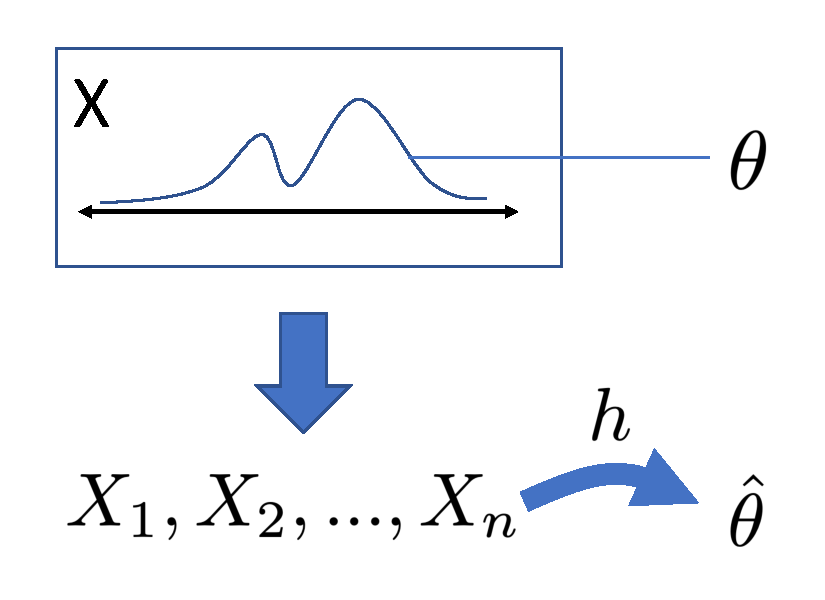
\includegraphics[width=0.5\linewidth]{images/estimator}}
    \note[item]{We can't observe the joint distribution directly, so
      we try to make guesses about it.} 
    \note[item]{An estimator could be any function of the statistic.
      Here, we'll pass the data through function h and get estimator
      $\hat{\theta}$.  This could be any function, but really, we
      want $\hat{\theta}$ to be a good guess for $\theta$}
\end{frame}

\begin{frame}
  \frametitle{$\overline{X}$ is an Estimator}
  We refer to statistics that are ``good'' guesses for a population parameter as
  \textbf{estimators}. 
  \begin{itemize}
  \item $\theta = \E[X]$ is a parameter.
  \item$T_{(n)} = \text{choose the 30}^{th} \text{ percentile}$ is a statistic
  \item $\hat \theta = \overline{X}$ is an estimator for $\theta$.
  \end{itemize}
\end{frame}

\begin{frame}
  \frametitle{Introducing Estimators}
  In this section, you will learn about the properties that make
  estimators good guesses for a population parameter.
  \begin{block}{Properties of estimators}
  \begin{itemize}
  \item \textbf{Consistency:} As sample size grows, does the estimator
    converge in probability to the true value? 
  \item \textbf{Bias} and \textbf{unbiasedness}: Is the estimator systematically too low or too
      high?
  \item \textbf{Efficiency:} Does an estimator have relatively
    \textit{large or small} sampling variance, standard error, and
    MSE? 
  \end{itemize}
  \end{block}
  \note[item]{\textbf{Consistency} Even if it is far from the truth in
    small samples, as $n$ increases, does an estimator $\hat{\theta}$
    get closer to the true value?}
  \note[item]{\textbf{Bias}: Across samples of any size, is an estimator
    systematically too low or too high?}
  \note[item]{\textbf{Efficiency}: Does a particular estimator have a
    relatively large or small mean squared error or sampling variance?
    If we have two estimators that are both unibased and consistent,
    I'd rather use the one that is closer to the truth on average.}   
\end{frame}

\section{Reading: Core Estimation Theory} 

\begin{frame}
  \frametitle{Reading: Core Estimation Theory}
  \textbf{Note: This is a READING CALL, just placing it here
    for organization.}
  Read pages 102–105, stopping at 3.2.3, Variance Estimators.
\end{frame}

\section{Desirable Properties of Estimators}

\begin{frame}
  \frametitle{Desirable Properties of Estimators}
  Throughout, we refer to $\theta$ as a population \textit{feature}
  or \textit{parameter}.
  \begin{itemize}
  \item $\theta$ has a fixed, true value, but this value is not
    directly observable.
  \note[item]{Examples of $\theta$: sentiment in a user population;
      donations to senate campaigns; mean age of MIDS instructors}
  \item Without ground truth, how can we know if our estimator is
    doing its job?
  \end{itemize}
  \note[item]{Test-driven development, engineering,
    analogy -- software teams imagine every scenario possible, write
    a testing suite -- and conduct tests before releasing. That's
    how they know it ``works''. Because we don't know $\theta$ we
    can't do the same.}
  % \note[item]{\paul{Just to push on your
  % analogy a bit... it made me think of simulation studies, like
  % we did to see how efficient the classical and robust
  % estimators for ols error are.  That seems to be a bit like the
  % software approach}}
  % \note[item]{\alex{I agree! Let's not bring this up to the students just yet
  %   though.} }
  \note[item]{Reasoning and evaluating these properties is one of the
    reasons that we have invested in probablity theory!}  
\end{frame}

\begin{frame}
  \frametitle{Desirable Properties of Estimators: Unbiasedness}
  \begin{block}{Bias of an estimator}
    \note[item]{The bias of an estimator is the difference between the
      truth, and what you estimate. In this way, the term
      \textit{bias} has the same meaning as our plain-language
      meaning.}
    \note[item]{However, we cannot use it
      \textit{unthinkingly}. People say in plain language, ``They got
      biased treatment,'' and, ``It was a biased process.'' I suspect
      what they mean to say, ``They got prejudiced treatment.''}
    \note[item]{Notice also that in order to evaluate whether an
      estimate is biaesd, we \textit{need} a concept of what the true
      value is.} 
    The bias of an estimator is the expected difference between the
    \textit{true} population value and the estimator.
    \begin{itemize}
    \item The \textit{bias} of $\hat{\theta}$ is $\E[\hat{\theta}] -
      \theta$.
    \item If $\E[\hat{\theta}] = \theta$, then there is no bias, and
      the estimator is \textit{unbiased}.
    \end{itemize}
  \end{block}
\end{frame}

\begin{frame}[t]
  \frametitle{Desirable Properties of Estimators: Unbiasedness (cont.)}
    If $\hat{\theta}$ is unbiased, does that mean that, for any sample
  taken, the estimate produced by $\hat{\theta} = \theta$?
  \begin{itemize}
  \item $\hat{\theta}$ as an \textit{estimator} is a random variable.
  \item The value that it takes on given a sample is the
    \textit{estimate}. 
  \end{itemize}
  \note[item]{Draw an unbiased estimator!} 
  \note[item]{As a RV, $\hat{\theta}$ has a set of values that it can
    take on, and a probability distribution about those values.}
  \note[item]{The \textit{estimator}, $\hat{\theta}$ is unbiased if
    its expected value, $E[\hat{\theta}]$ is the same as the truth.}
  \note[item]{Draw a biased estimator!}
  \note[]{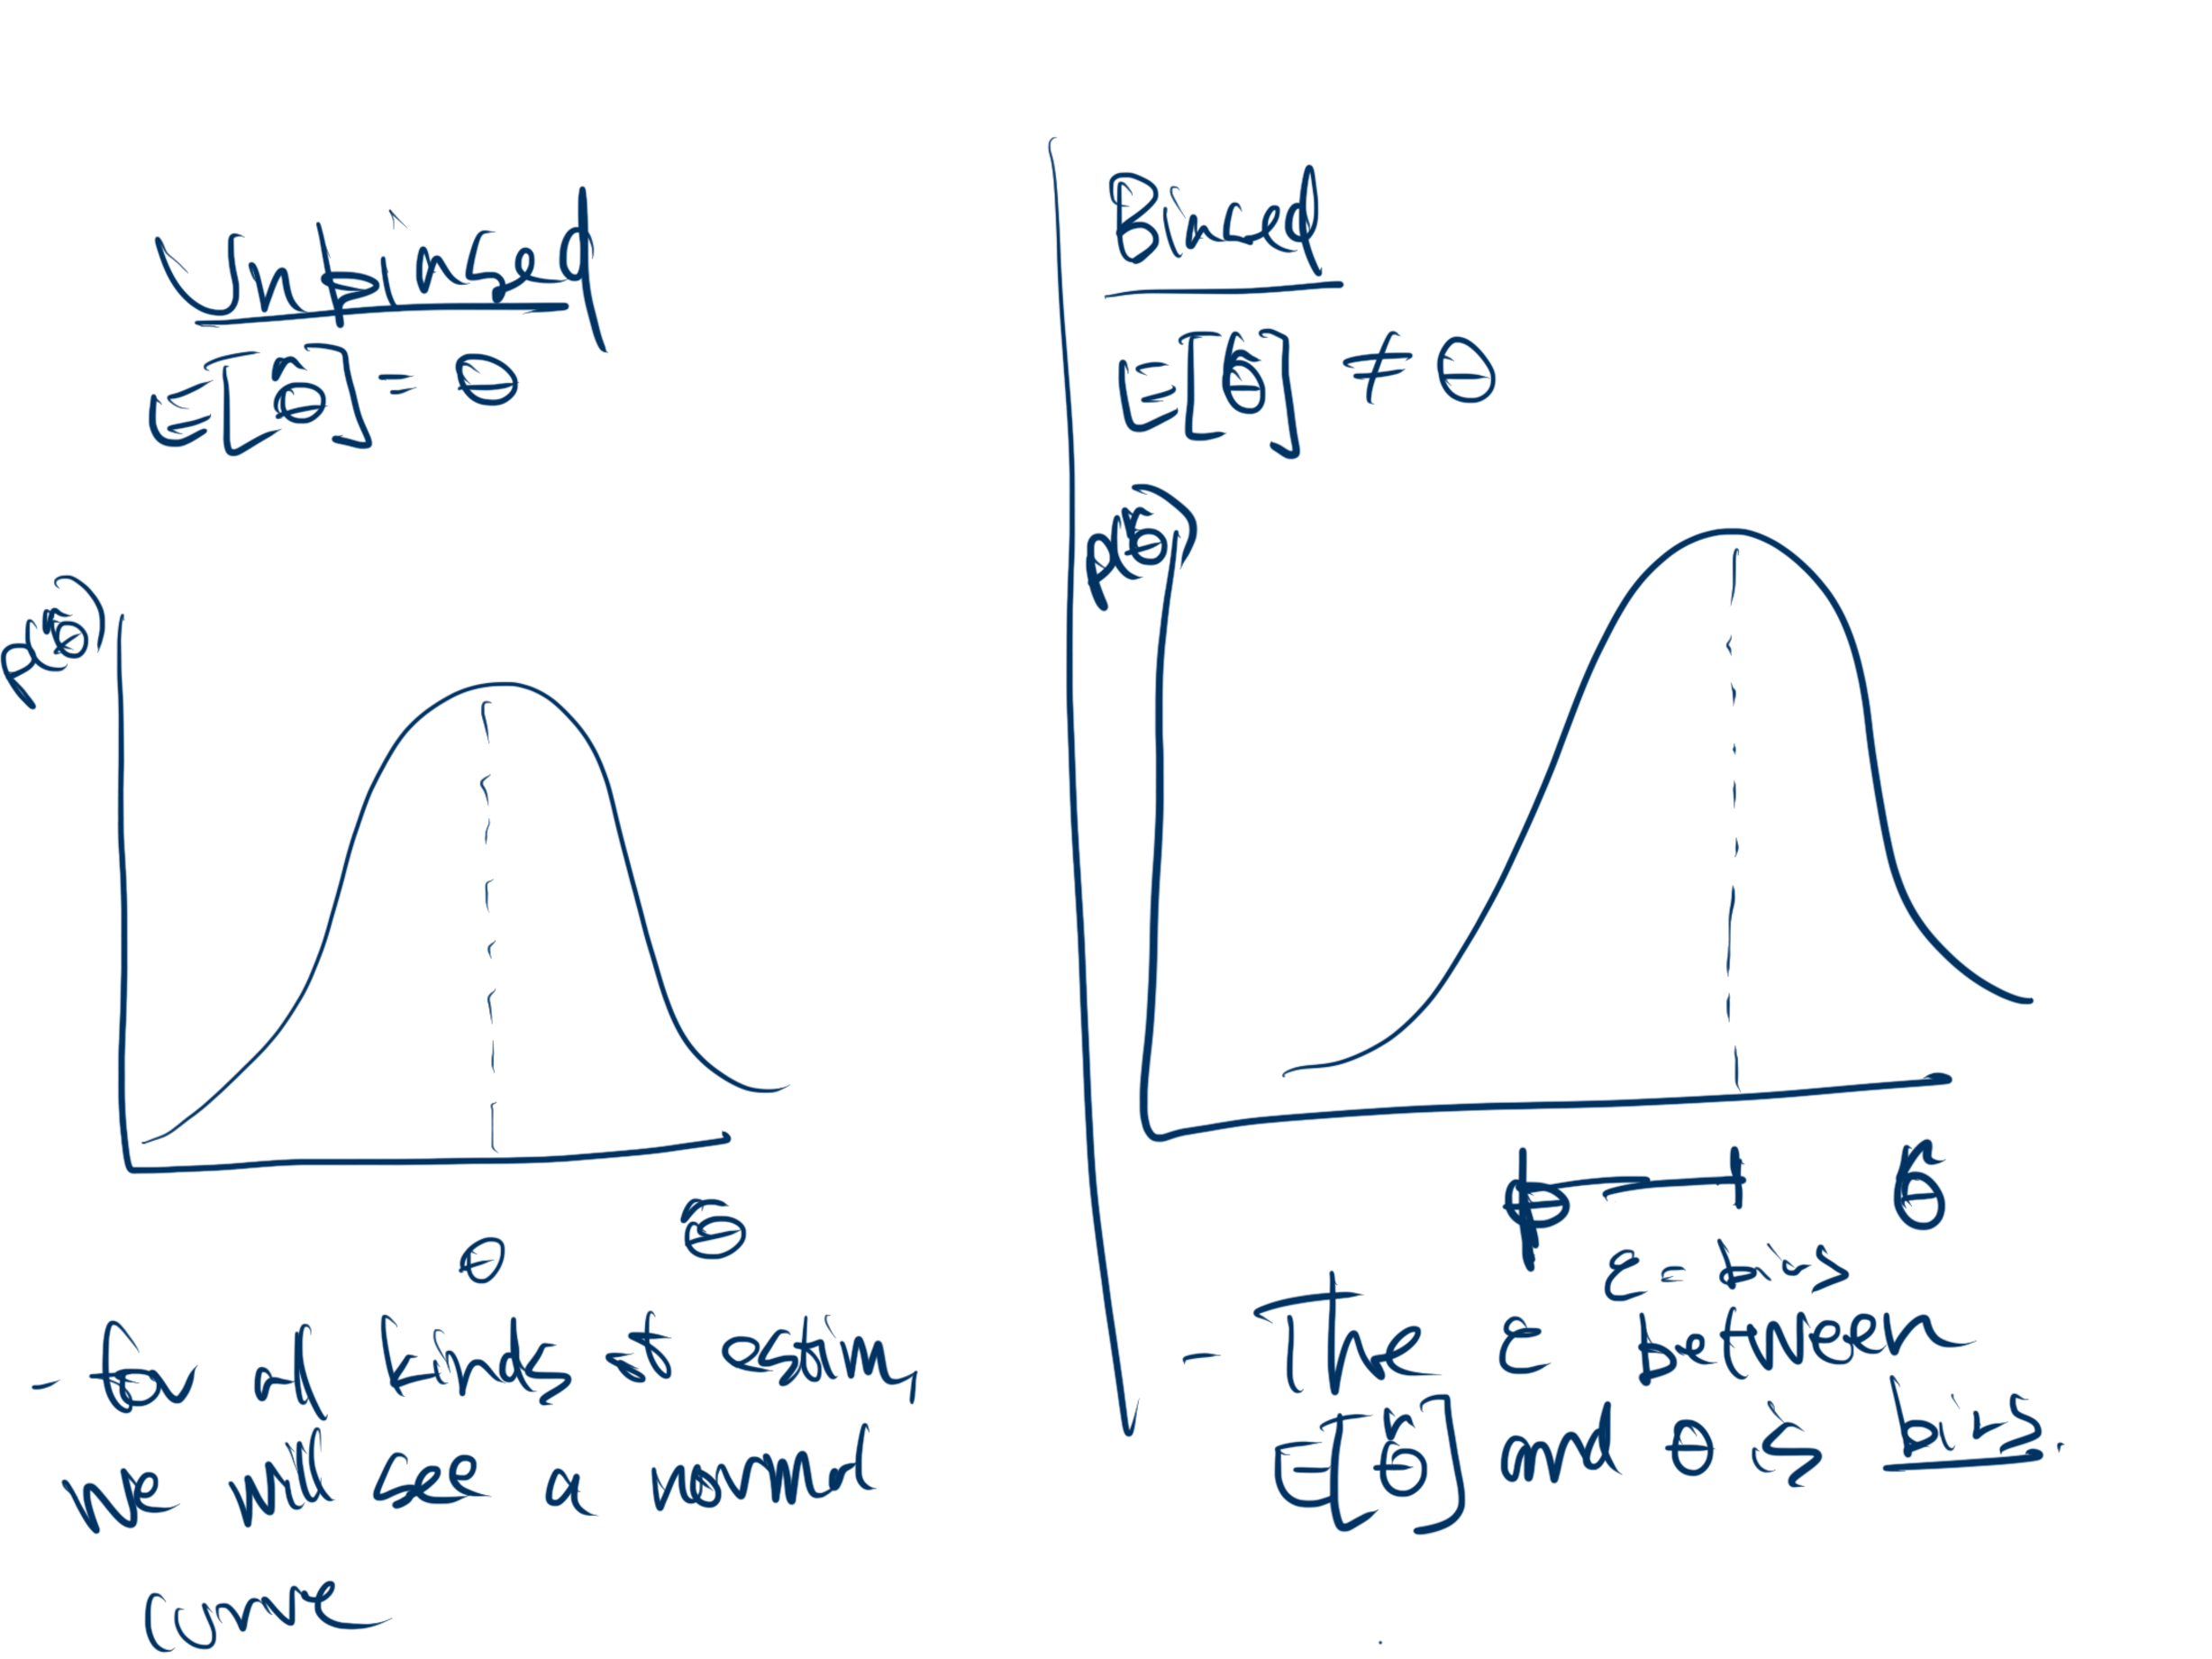
\includegraphics[width=0.5\linewidth]{./images/unbiased_estimator}}
\end{frame}

\begin{frame}
  \frametitle{Desirable Properties of Estimators: Unbiasedness
    (cont.)}

\end{frame} 

\begin{frame}[t]
  \frametitle{Desirable Properties of Estimators: Efficiency}
  \begin{block}{Mean Squared Error of an Estimator}
    \begin{itemize}
    \item The MSE of an estimator  $\hat{\theta}$ is
      \[
        E[(\hat{\theta} - \theta)^{2}] = V[\hat{\theta}] +
        (E[\hat{\theta}] - \theta)^{2}
      \]
    \end{itemize}
  \end{block}
  \note[item]{Suppose you are taking temperature, and have two
    methods: (1) back of hand; (2) under-tongue. Which would you
    prefer?}
  \note[]{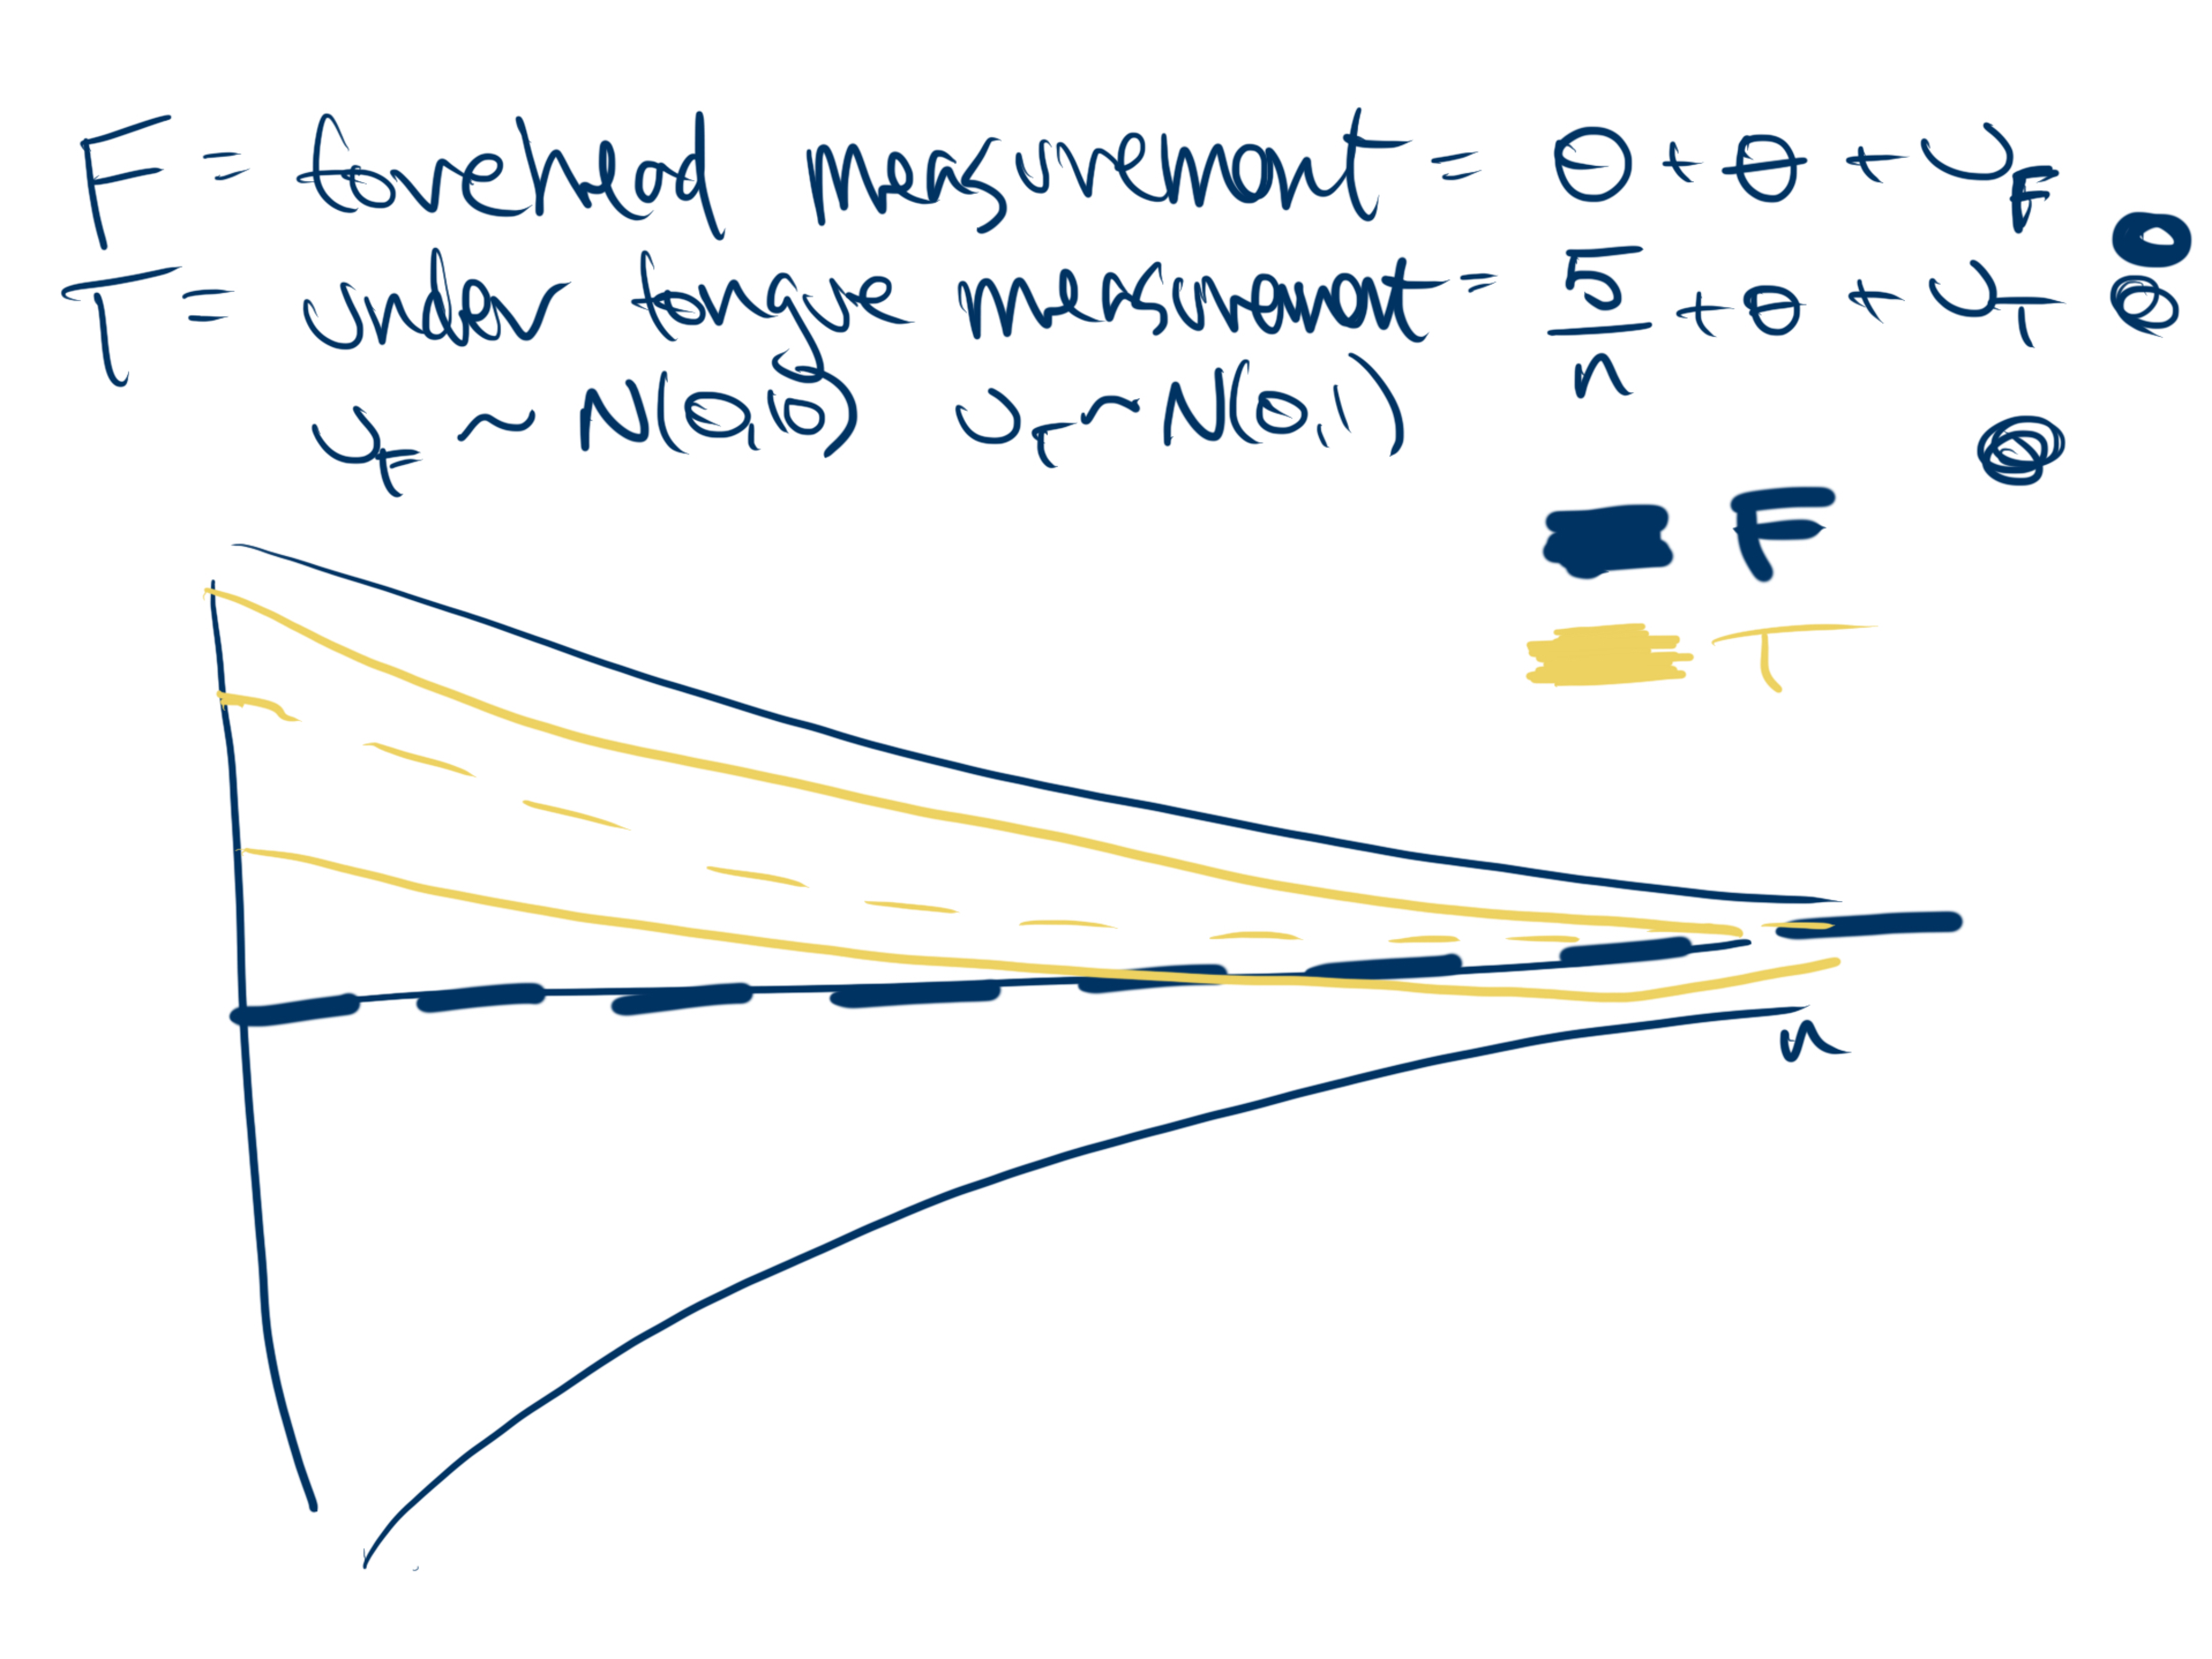
\includegraphics[width=0.7\linewidth]{./images/relative_efficiency}}
\end{frame}

\begin{frame}
  \frametitle{Desirable Properties of Estimators: Efficiency}
  
\end{frame}

\begin{frame}[t]
  \frametitle{Desirable Properties of Estimators: Consistency}
  \begin{block}{Consistency}
    An estimator $\hat{\theta}$ is consistent for $\theta$ if
    $\hat{\theta}\overset{p}{\to}\theta$.
    \note[item]{If an estimator isn't consistent, then many times we
      would say it isn't worth using.} 
  \end{block}
  \note[]{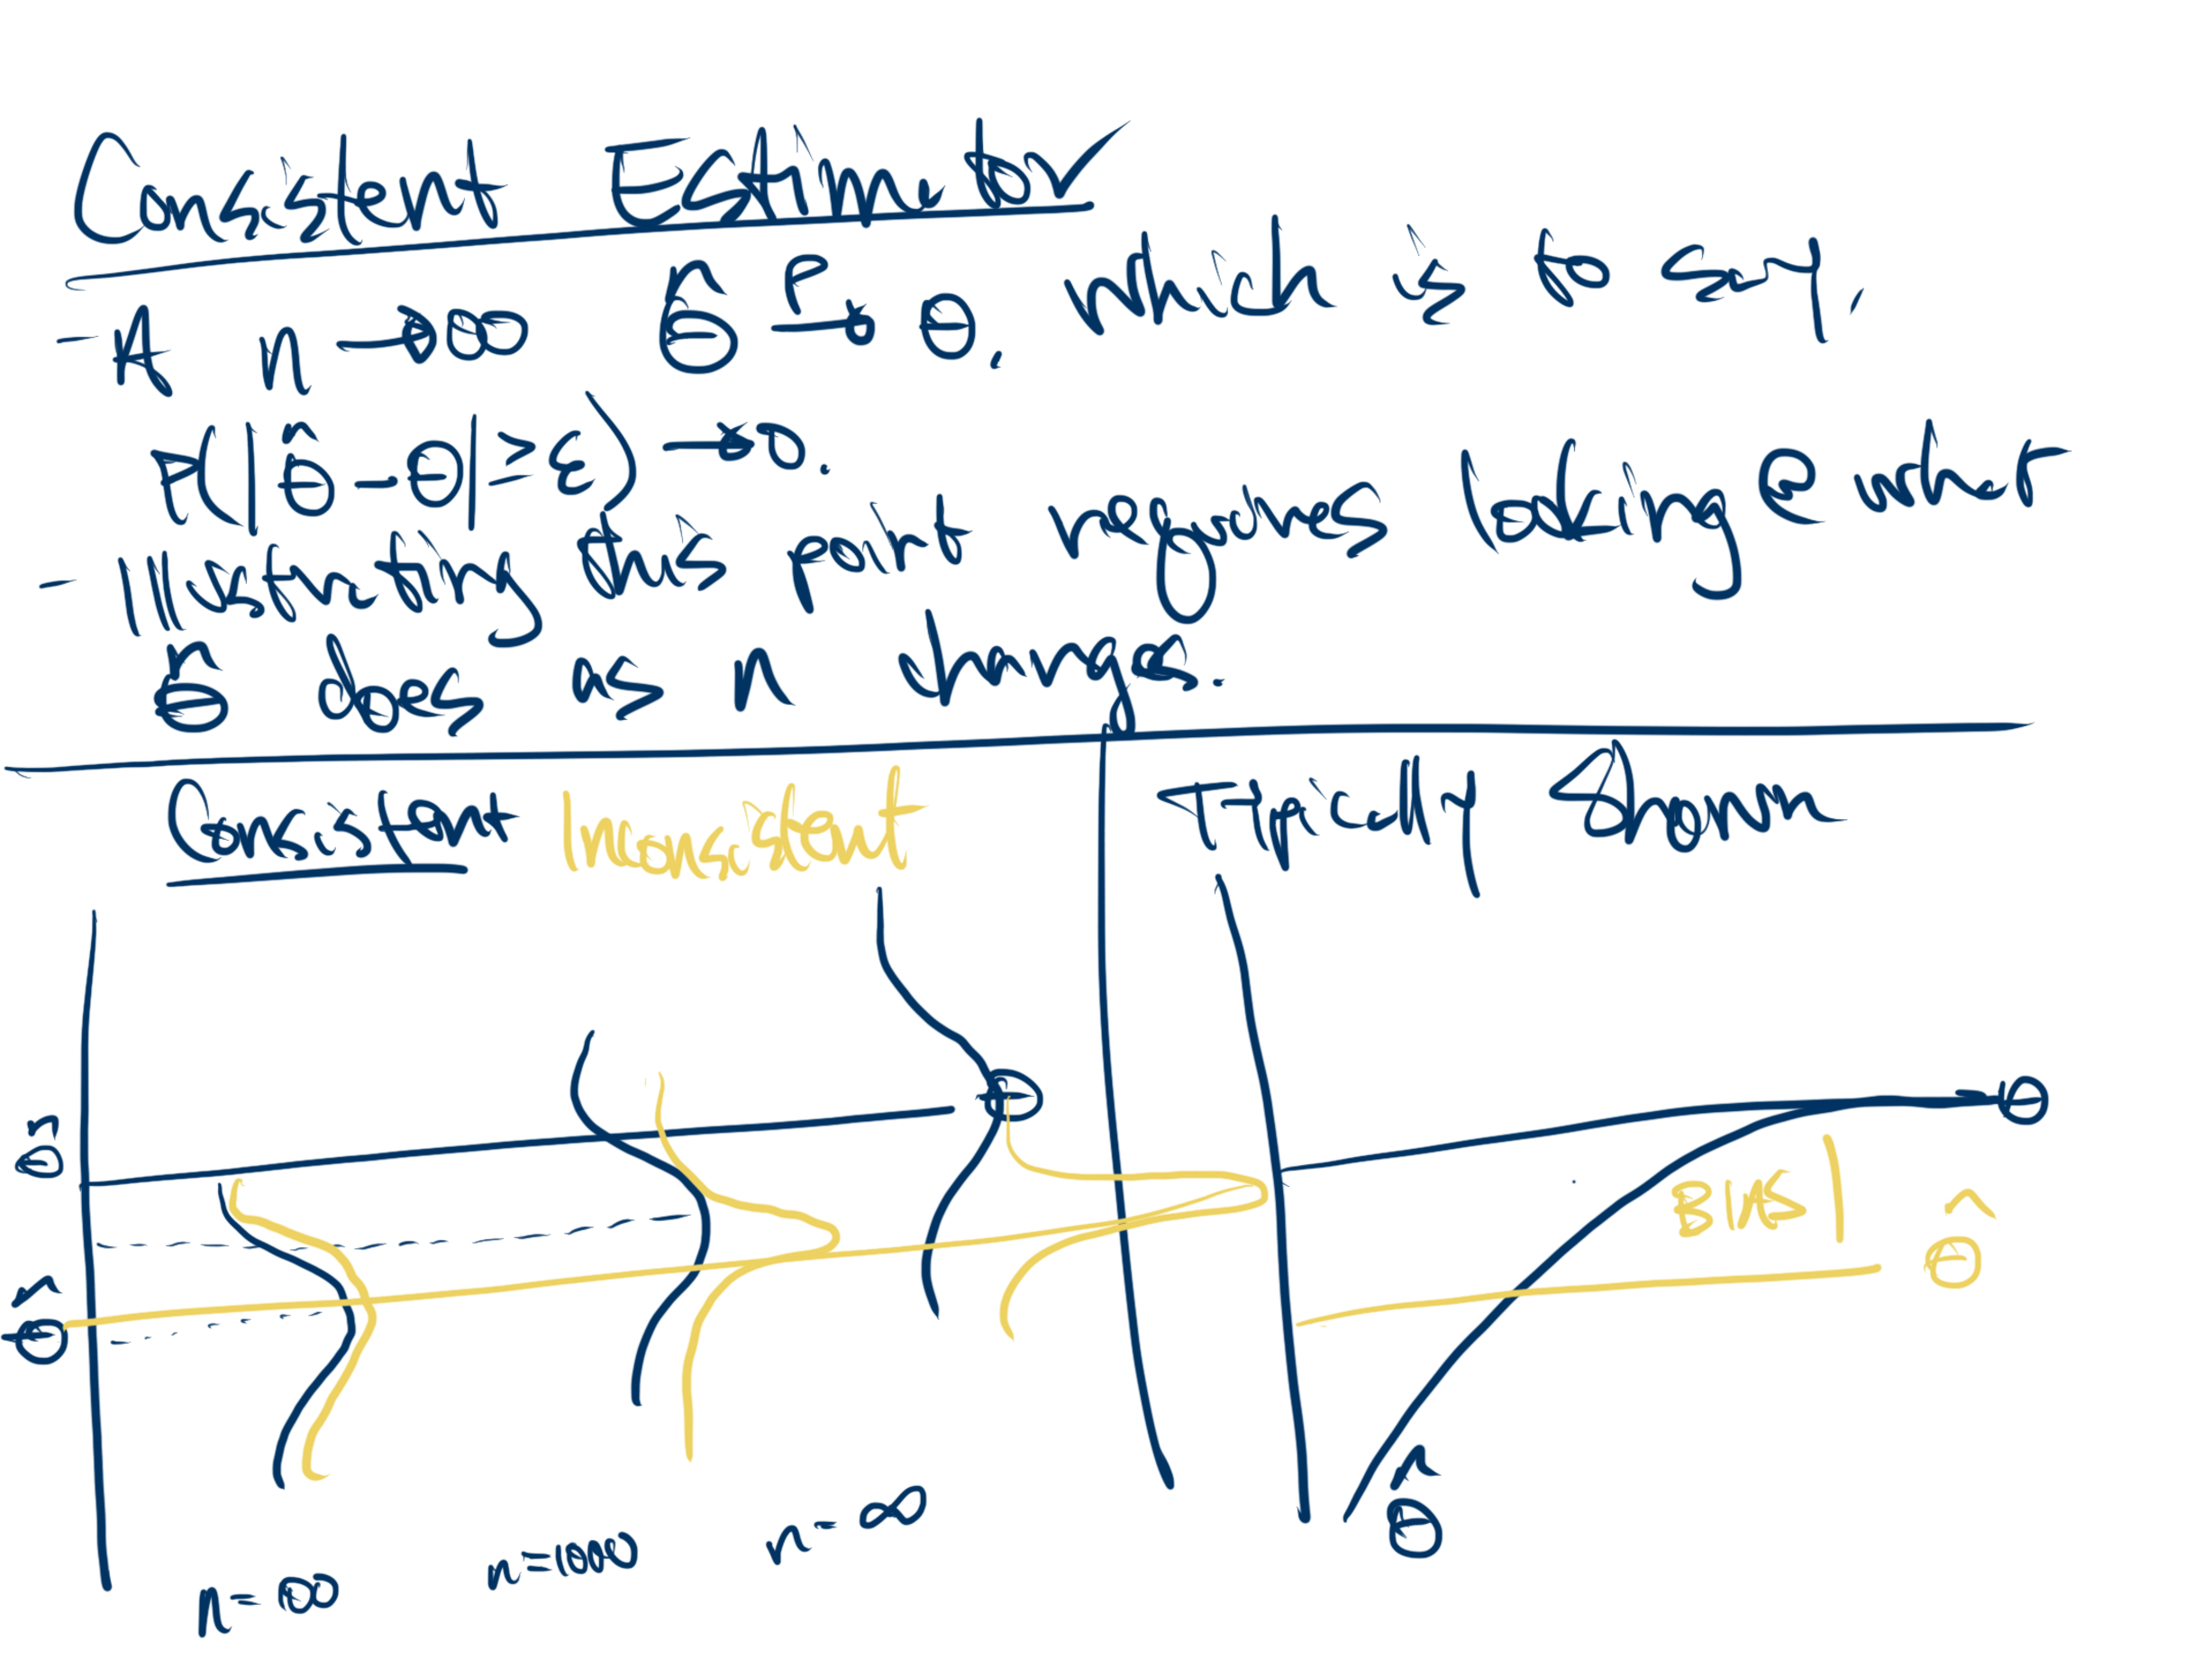
\includegraphics[width=0.8\linewidth]{./images/consistent_inconsistent}}
\end{frame}

\begin{frame}
  \frametitle{Desirable Properties of Estimators: Consistency}
  
\end{frame}

\section{Applying Properties of Estimators} 

\begin{frame}
  \frametitle{Evaluating Estimators}
  Which do you prefer? 
  \note[item]{Draw two estimators: (1) sine in n -- wavvy; (2)
    typically converging}
  \note[]{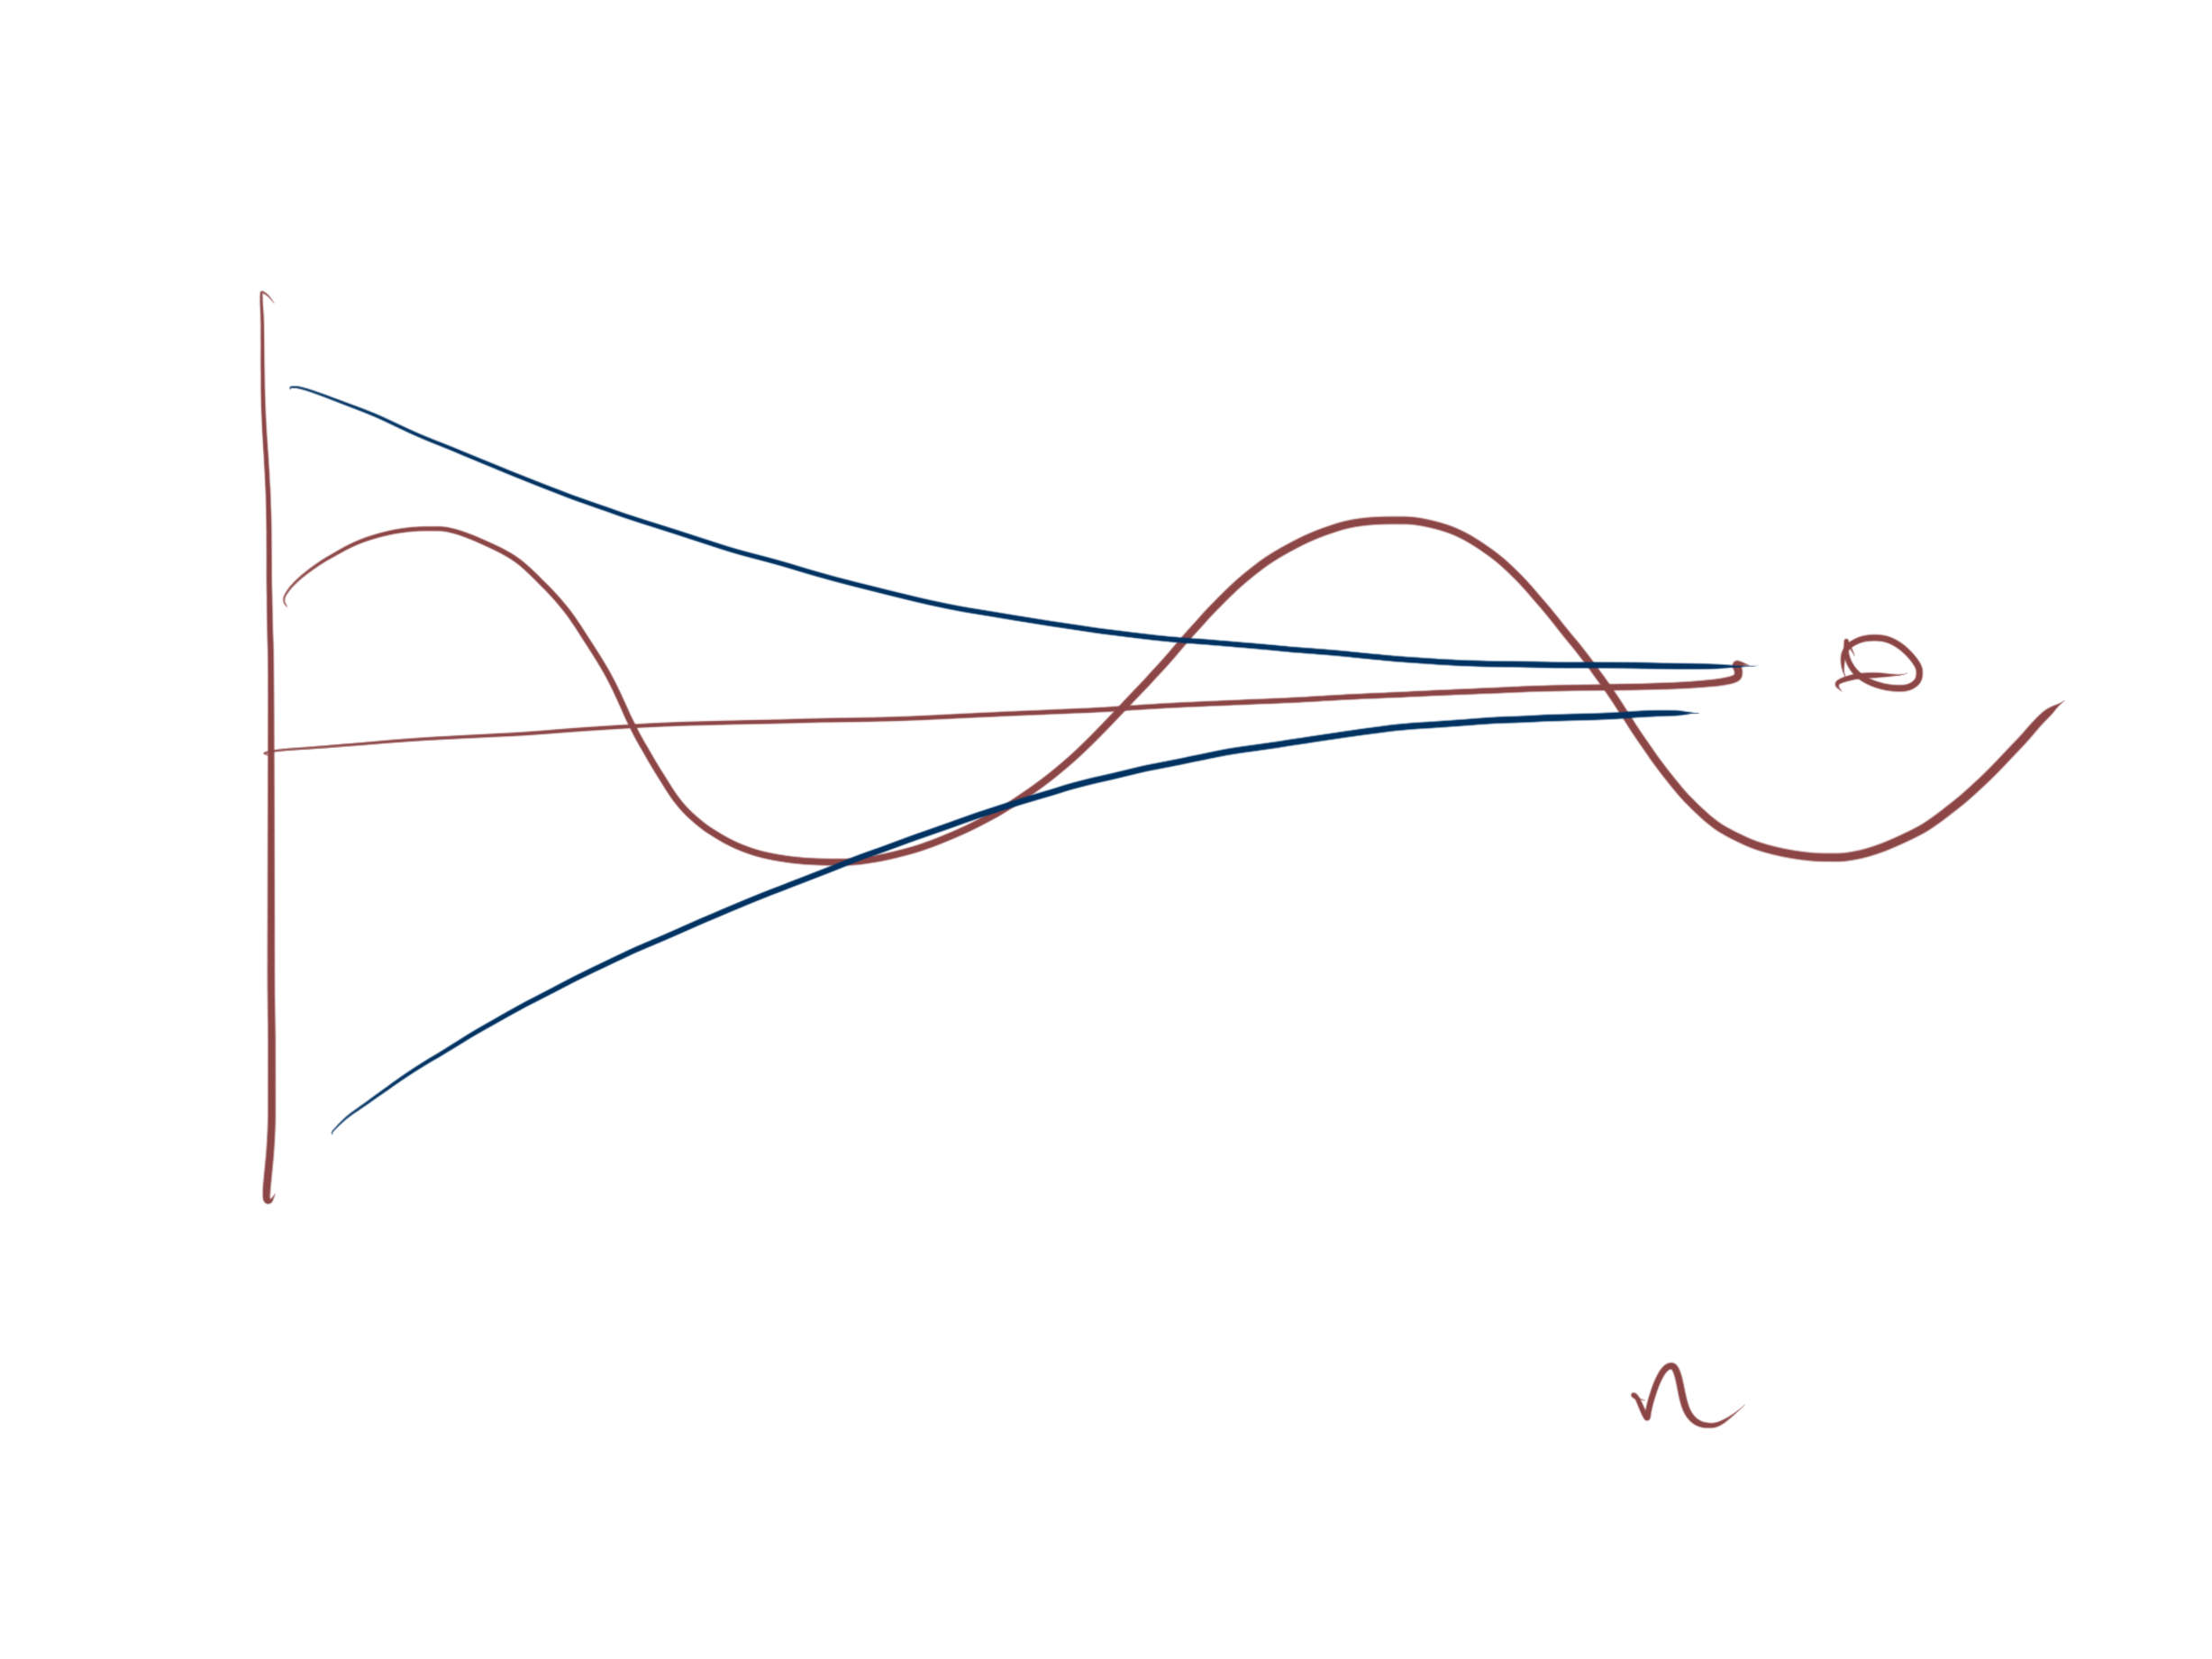
\includegraphics[width=0.7\linewidth]{images/evaluating_estimators_i}}
\end{frame}

\begin{frame}
  \frametitle{Evaluating Estimators (cont.)}
  \note[item]{Draw two estimators}
  \note[item]{Make both be consistent, one that is relatively more
    efficient.}
  \note[]{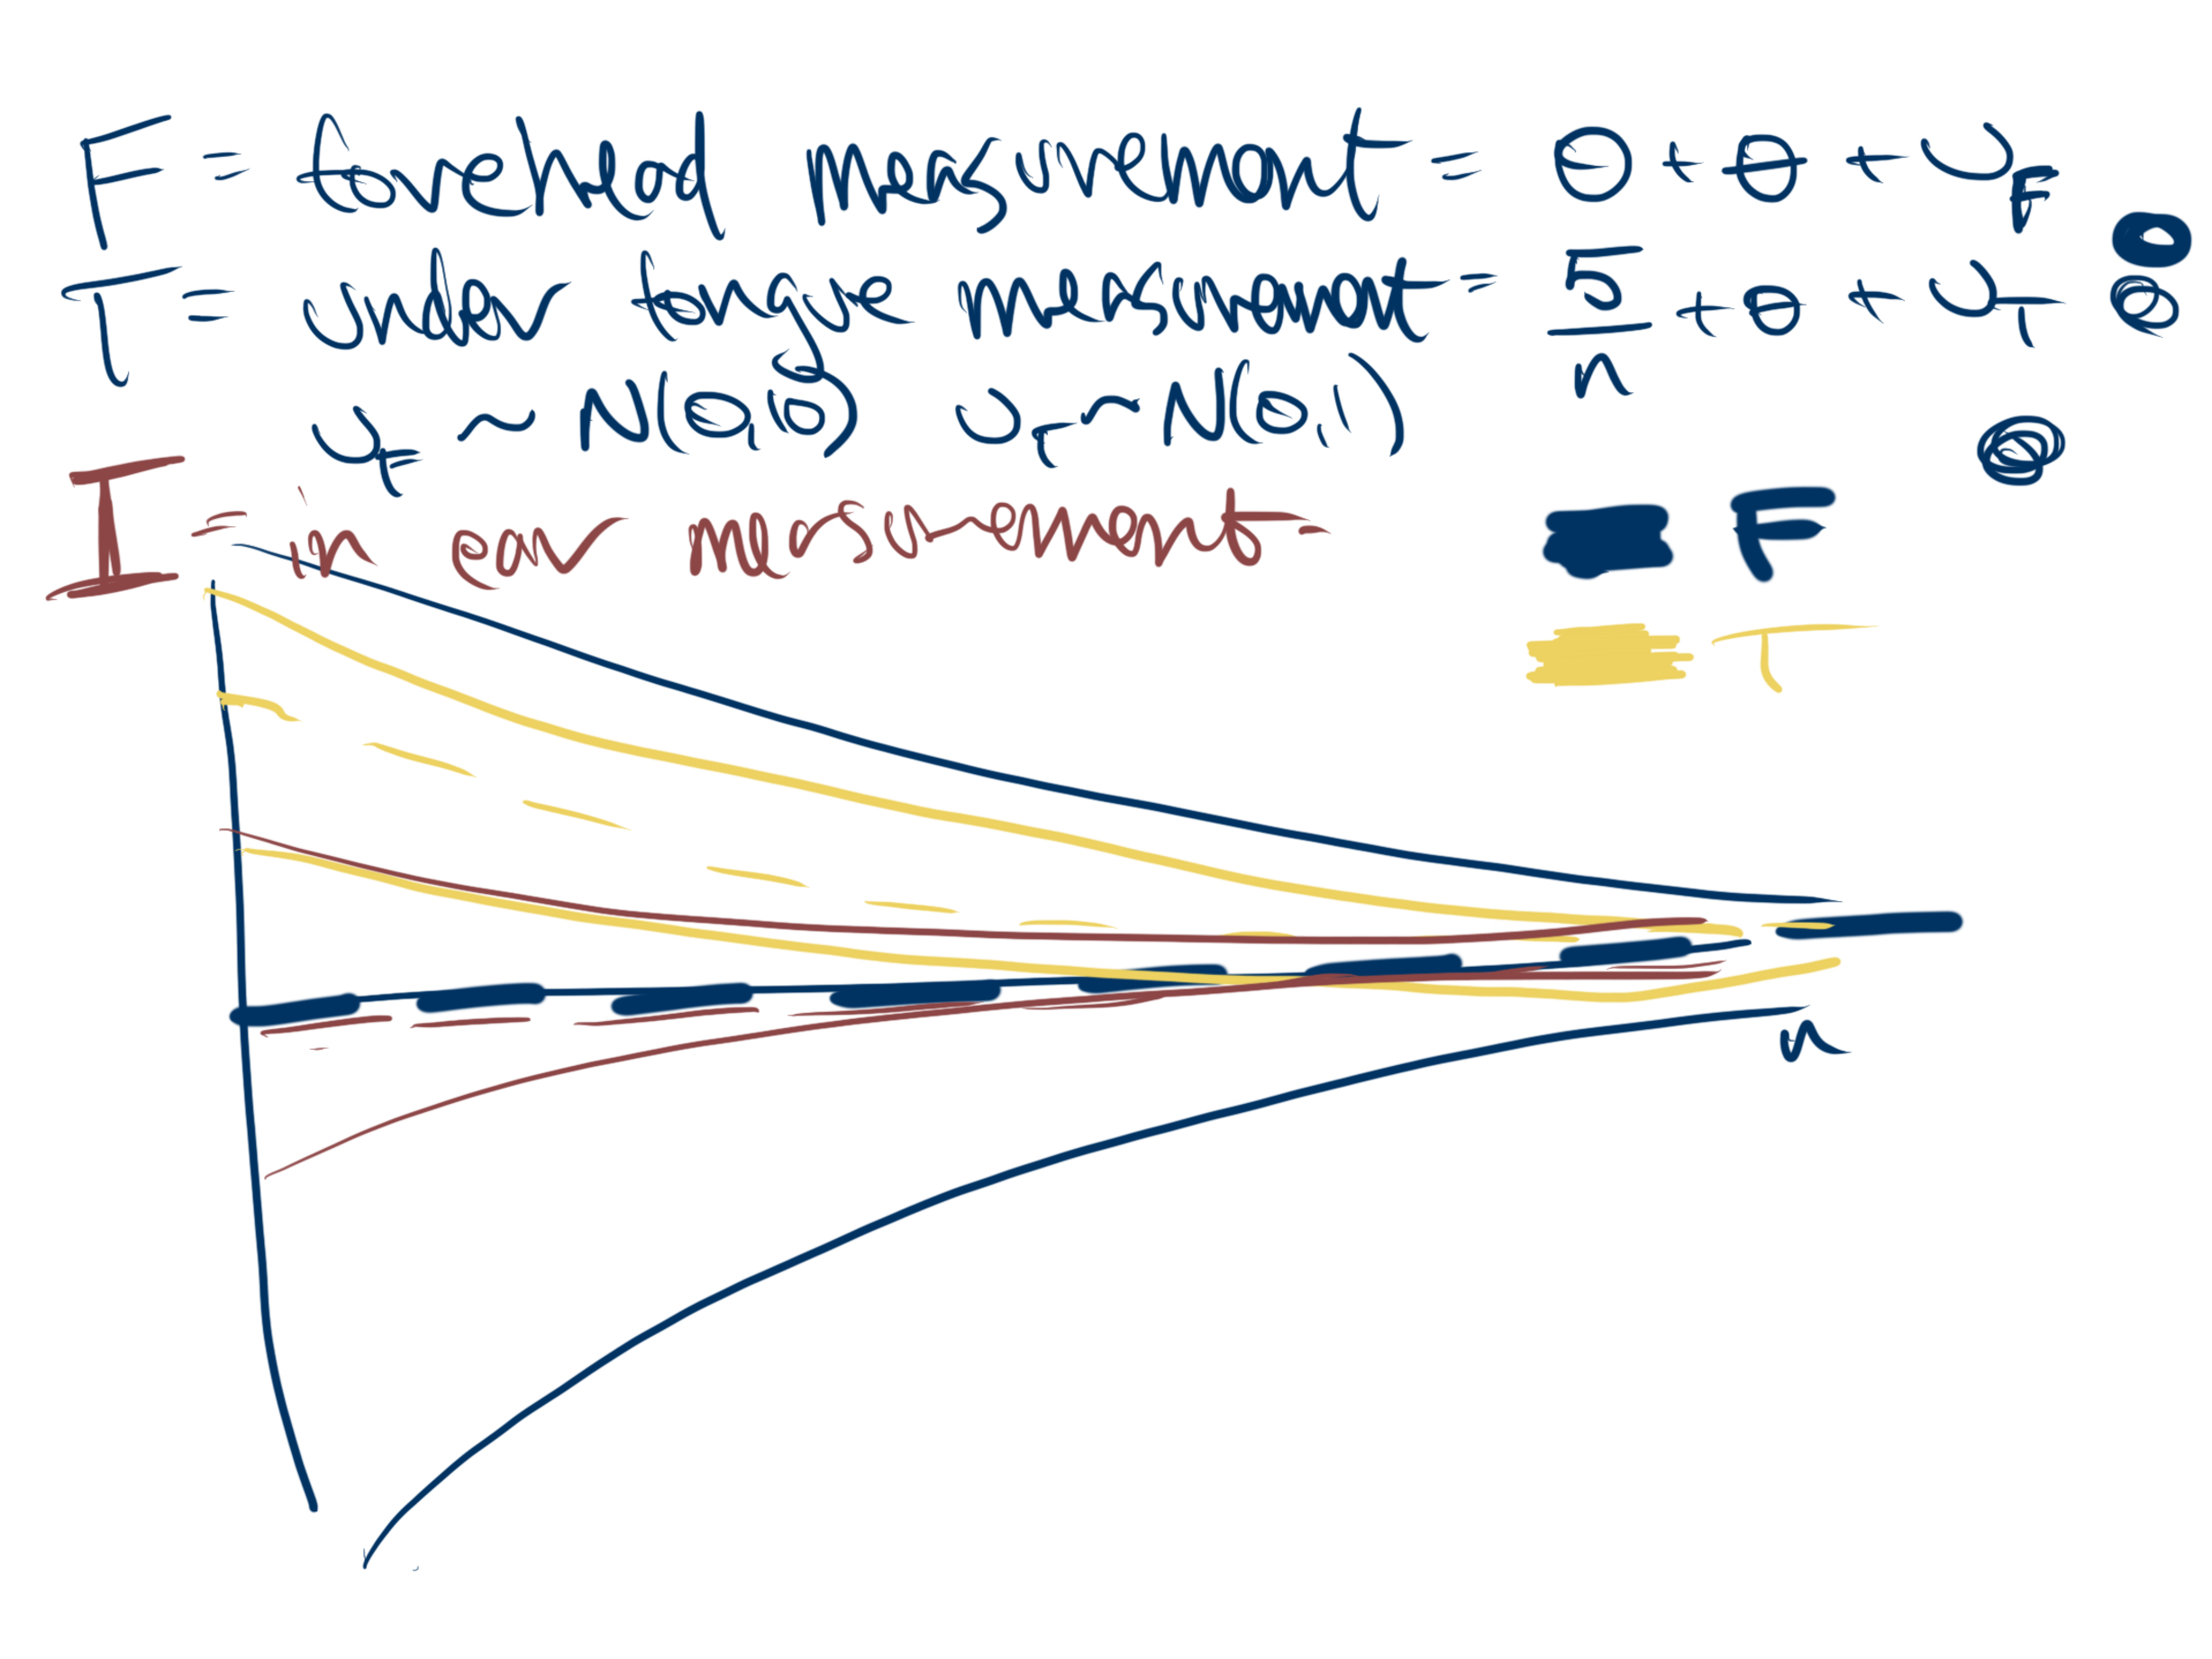
\includegraphics[width=0.7\linewidth]{images/evaluating_estimators_ii}}
\end{frame}

\begin{frame}
  \frametitle{Desirable Properties of Estimators: Review}
  \begin{itemize}
  \item An \textit{inconsistent} estimator is of little use.
  \item A \textit{more efficient} is estimator is preferable to a
    \textit{less efficient} estimator, all else equal.
  \item An \textit{unbiased} estimator is preferable to a
    \textit{biased} estimator, all else equal.
  \end{itemize}
  \note[item]{For inconsistent estimators, perhaps there is some level
    of $n$ that you get lucky and get the parameter estimate
    correct. But, \textbf{you don't know what that level is!}}
  \note[item]{More efficient estimators are preferrable, all else
    equal. But, in a business context there \textit{has} to be a
    tradeoff between cost and efficiency. How precise do you need to
    be?}
\end{frame}


\section{Random Sampling}

\section{Reading: Independent and Identically Distributed}

\begin{frame}
  \frametitle{Reading: Independent and Identically Distributed}
  \begin{itemize}
  \item Read Section 3.0 and 3.1 in \textit{Foundations of Agnostic
      Statistics} (pages 91–96 in our copy of the book.)
    \begin{itemize}
      \item Work to place the formal math definition into plan
        understanding. We will discuss this when you come back.
      \item Notice how $\mu$ and $\sigma^{2}$ are concepts that are
        immediately familiar, but they now represent population
        parameters.
    \end{itemize} 
  \end{itemize}
  \note[item]{The mathematical formalism in \textit{Definition 3.1.1} is
    probably overkill; we will talk about it when we come back.}
  \note[item]{\textit{Definition 3.1.2 -- the Finite Population Mass
      Function shows how we could move from talking about actual
      people to random variables (but keep in mind that we will almost
      always assume an "infinite superpopulation".) }}
  \note[item]{Notice how $\mu$ and $\sigma^{2}$ are concepts that are
    immediately familiar, now these represent population parameters,
    rather than some abstract probability} 
\end{frame}
\section{Independent and Identically Distributed} 

\begin{frame}
  \frametitle{Independent and Identically Distributed}
  \begin{block}{Definition: independent and identically distributed (IID)}
    \begin{itemize}
    \item Undertake some process an arbitrary number of times—call
      it \textit{sampling}—to create a value from a phenomenon.
    \item If each instance of sampling draws from the same probability
      distribution, then we say the collection of values are
      \textbf{identically distributed}.
    \item If none of the instances of sampling provide information
      about other instances of sampling, then we say the collection of
      values are \textbf{independent}. 
    \end{itemize}
    \note[item]{Talk through the definitions first.}
  \end{block}
\end{frame}

\begin{frame}
  \frametitle{Independent and Identically Distributed (cont.)}
  \note[]{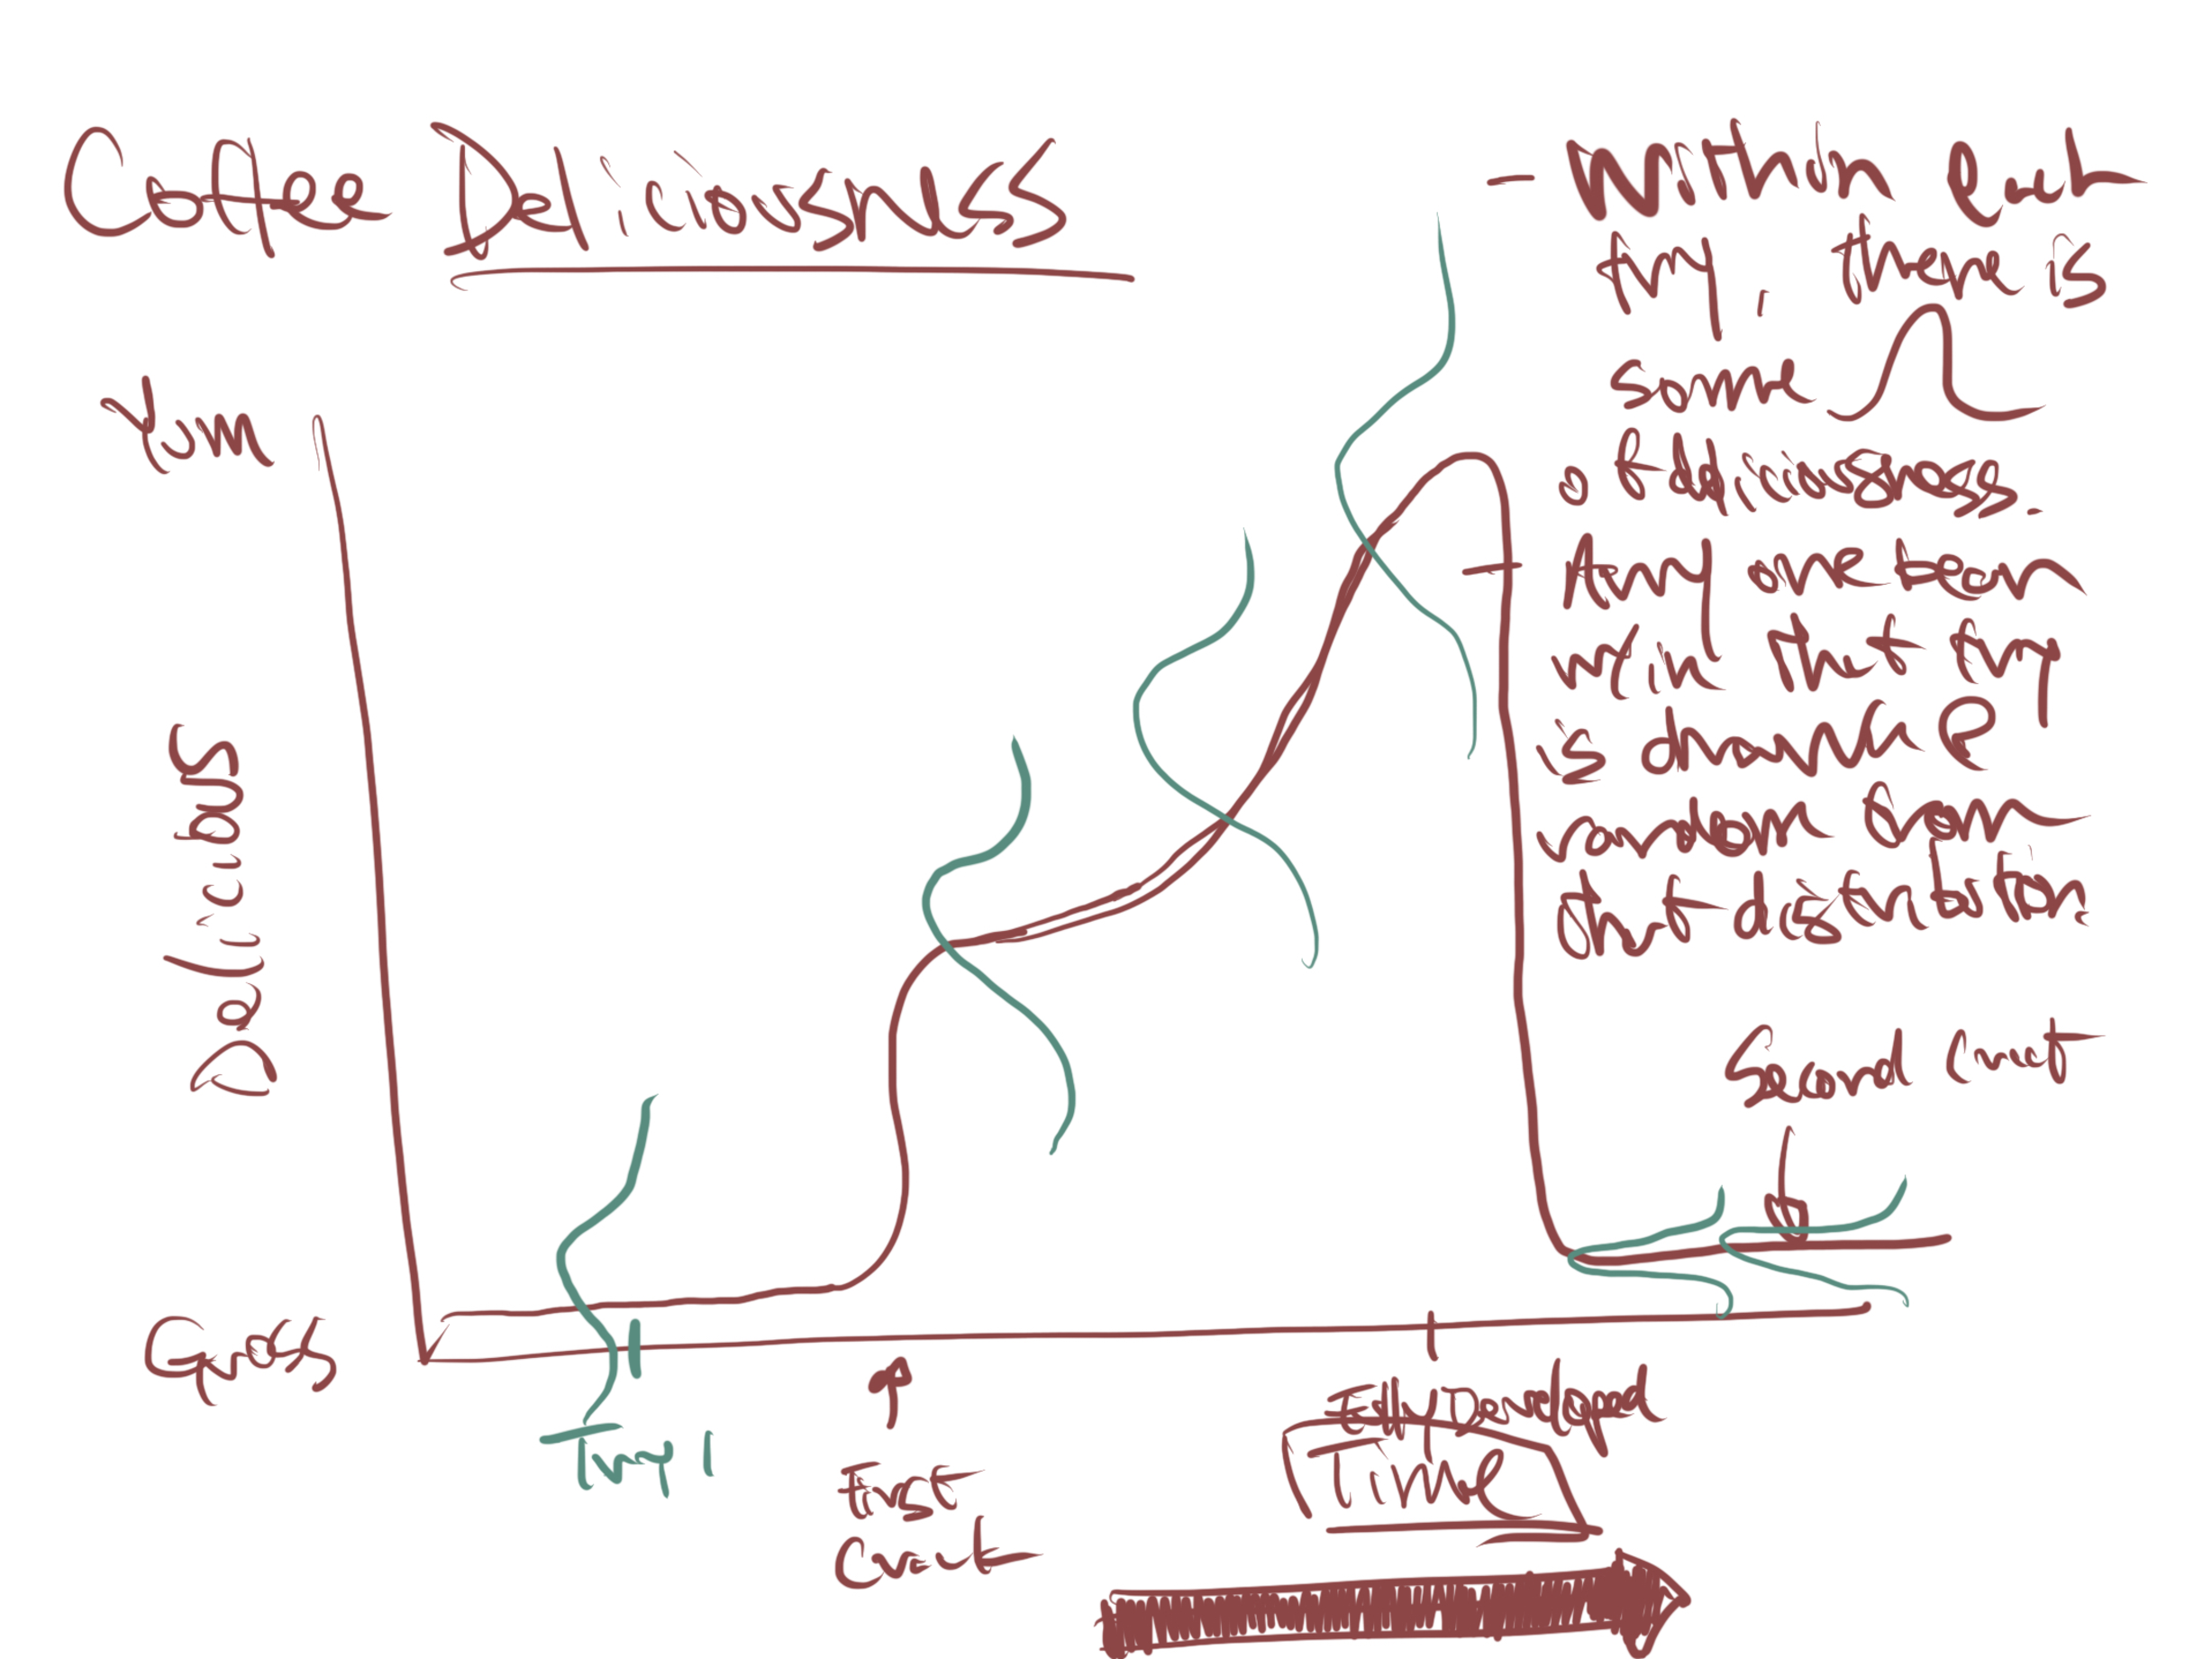
\includegraphics[width=0.5\linewidth]{./images/coffee_delicious}}
  \note[item]{Each of the sets of \textit{trys} draws 30 beans at
    ``random''. But, are these draws i.i.d? }
  \note[item]{Problem 1: We have a finite sample in this roaster --
    there are 10,243 beans in it. Paul counted! Ha! After we draw and
    look at one, there are only 10,242 left to draw, and we've changed
  the distribution of the beans by taking one out. So, technically, we
  have a dependent sampling process.} 
  \note[item]{But, subsequent ``trys'' are not independent. When I
    know how roasted each bean in try (3) is, I know that each bean in
    try (4) is going to be more roasted.}
  \note[item]{Problem 2: The beans only get \textit{more} roasted. Time
    only goes fowrard, and in doing so, each of the distributions are
    related to one another}
  \note[item]{Problem 3: Suppose you get one \textit{really} roasted
    bean in try 1. Does that mean that in try 2 you're going to get
    anothe really roasted bean? No! The distributions are no
    indepenent, but all of the tries are.}
  \note[item]{Problem 4: What if all the big beans ``float'' to the
    top and so get less heat? Then we would have a non-independent
    distribution!} 
  \note[item]{Problem here is that I don't think you can
      define a model where a very roasted bean in try 1 gives you
      information that beans in try 2 are likely to be more roasted,
      but not that the next bean in try 1 is likely to be more
      roasted.  Any way I think of it, either both pairs are
      independent or not independent.}
\end{frame}

\begin{frame}
  \frametitle{Making Assumptions}
  \begin{itemize}
  \item What is a statistical assumption? 
  \item When are they important? 
  \item When can I violate them? 
  \item What do I do if they are violated?
  \end{itemize}

  \note[item]{Up until this point, all of our work has been
    axiomatic.}
  \note[item]{We began with a principle, we looked at rules, and we
    observed what fell out.}
  \note[item]{Now we're stepping into the fun, but clumsy world that
    forces us to put these alabaster axioms to work.}
\end{frame}

\begin{frame}
  \frametitle{Making Predictions}
  \pause
  \note[item]{As data scientists, we might sometimes posess the entire
    universe of data and want to characterize it -- ``What is the
    sentiment of all the employees in \textit{this}
    department''.} 
  \note[item]{Much more frequently we're interested in something else
    -- making a statement about a population from limited data.}
  \note[item]{What sets statistics apart is that it attempmts to
    characterize how certain we are about these predictions.}
  \note[item]{Without IID, we might be incorrectly confident --
    leading to unforseen events. Or, we might learn someting about a
    population that isn't informative of our target.}
  \begin{itemize}
  \item When data are independent and identically distributed (IID), it is possible to learn desirable things from
    a sample:
    \begin{itemize}
    \item Accurate characterizations of the probability distribution
      function and values 
      \item Reliable characterizations of certainty and
        uncertainty
      \end{itemize}
    \item We can learn about unseen \textit{population parameters}
      from a sample and then use our domain knowledge to evaluate
      whether these population parameters apply to some circumstance. 
  \end{itemize}
\end{frame}

\begin{frame}
  \frametitle{What Is a Population?}
    
  \note[]{When we model data as draws from a random variable $X$, we call $X$
  the population.}
  \note[item]{$X$ may be finite, but this is less common than you
    think.}
  \begin{block}{U.S. Senator fundraising}
    There are 100 U.S. Senators.
    \begin{itemize}
      \item One could reason about a finite population with 100
        elements.
        \note[item]{Then, we \textit{know} the whole population, and
        there is nothing to estimate.}
      \item Or, one could assume a continuous distribution for
        fundraising.
        \note[item]{Each senator is a draw from this distribution.}
        \note[item]{If we are interested in fundraising \textit{in
            general} this lets us say things about the \textit{next
            set of senators}, not only the 100 who happen to be there
          now.}
        \note[item]{We know the idea of this joint distribution of an
          infinite number of senators is strange, but (a) look at how
          it broadens the questions we can answer; and (b) this is how
          statisticians reason about the world.}
    \end{itemize} 
  \end{block}  
\end{frame}


\section{Learnosity: Is This IID?}

\begin{frame}
  \frametitle{Is This IID? }
    \textbf{Note: This is a learnosity activity, just placing it here
    for organization.}

  For each of these, would you say that this sample is distributed
  IID? What do you understand about the process that brings you to
  your conclusion? 
  \begin{itemize}
  \item Coffee
    \begin{itemize}
    \item \textbf{Goal:} Understand how roasted a batch of coffee is.
    \item \textbf{Sampling process:} Dip into a drum to pull a set of 30 beans. 
    \end{itemize}
  \item Conduct a draft
    \begin{itemize}
    \item \textbf{Goal:} Randomly select people for military service.
    \item \textbf{Sampling process:} Draw balls from an urn with a day
      of the year. Everybody born on that day goes to war. 
    \end{itemize}
      \item Produce training data for machine vision 
    \begin{itemize}
    \item \textbf{Goal:} Gather images of normal and abnormal cellular
      structures to train neural net to recognize cancerous cellular structures.
    \item \textbf{Sampling process:} Randomly select 10 patients (with
      consent!) from the general outpatient population (unlikely to
      have the cancer), and randomly select 10 patients (with
      consent!) from the oncology department (that are likely to have
      the cancer).
    \end{itemize} 
  \end{itemize}
\end{frame}

\begin{frame}
  \frametitle{Is This IID? (cont.)}
  \begin{itemize}
    \item Teach a computer to \textit{really} read
    \begin{itemize}
    \item \textbf{Goal:} Teach a computer to understand theme and plot
      (the work of School of Information professor David Bamman).
    \item \textbf{Sampling process:} Feed a neural network each word
      (in each sentence [in each paragraph (in each chapter)]) of the English
      language literary canon.
    \end{itemize}
  \item Any others?
    \begin{itemize}
    \item \textbf{Goal:} 
    \item \textbf{Sampling process:} 
    \end{itemize}
  \end{itemize}
\end{frame}

\section{Reading: Sample Statistics}

\begin{frame}
  \frametitle{Reading: Sample Statistics}
  \begin{itemize}
  \item Read pages 96–98.
  \item Stop before theorem 3.2.5.
  \end{itemize} 
\end{frame}

\section{Sample Statistics}

\begin{frame}
  \frametitle{Sample Statistics}
  Sample statistics are:
  \begin{itemize}
  \item Functions that are applied to samples of random variables
    \note[item]{Why do we say that $X_{1}, X_{2}, \cdots, X_{3}$ are
      all random variables and not just realizations of a random
      variable?}  \note[item]{Make clear that sample statistics are
      \textbf{any} function of a random variable. Some are more useful
      than others, but they are just any mapping from
      $\mathbb{R}^{N} \rightarrow \mathbb{R}$ space} \note[item]{There
      are some \textit{classics} that we'll cover right now -- sample
      average, variance and standard error -- but also ranks, splines,
      factor loadings, space embeddings}
  \item \textit{Themselves} random variables
  \end{itemize}
    \note[item]{At this point, we don't have any guarantee about what
      the sample statistics will look like under repeated sampling. If
      you've taken a stats course before, though, you'll recognize
      that we're building towards  sampling distribution of these statistics.}
\end{frame}

\section{Conduct Sampling}

\begin{frame}
  \frametitle{Conduct Sampling}
  \textbf{Note: This is a learnosity activity, just placing it here
    for organization.}

  The goal is that this will solidify the understanding that students
  have from the reading and will move us forward into a conversation
  about expected value and the sample variance of the sample average.
  
  \begin{itemize}
  \item Students will be provided with data and starter code that
    produces a population. 
  \item From this population, they will have sliders they can
    pull that will increase or decrease the number of samples that
    they take, the number of draws per sample, and the underlying
    population variation.
  \end{itemize}
  
\end{frame}

\section{The Sample Mean as an Estimator}

\begin{frame}
  \frametitle{The Sample Mean}
  \begin{block}{Definition: Sample Mean}
    For IID random variables, $X_1,..X_n$, the \textit{sample mean} is
    \[
      \overline{X} = \frac{1}{n}\sum_{i = 1}^{n}X_{i}
      \] 
    \end{block}
    
    \begin{itemize}
\item The sample mean is an \textit{estimator} for $\E[X]$.
\end{itemize}

    \note[item]{Let's dive into out first example of an estimator: the sample mean.}
    \note[item]{I'm sure you've taken thousands of means in your life, but you might not have thought of the sample mean as an estimator.}
    \note[item]{First, what kind of object is this?  It's a statistic.  It's a function of a sample, which is made up of random variables, so it is a random variable.  This is really our statistical model that describes how a sample mean you write down in your analysis gets there.}
    \note[item]{As statisticians, we're not really interested in the sample mean for its own sake.  We're interested in the population mean.  We're using the sample mean, because it's an estimator for the population mean.}
%    \note[item]{Notice, immediately, the similarity to the Expected
%      value operator.}
%    \note[item]{This is a common theme -- we have a concept that
%      operates in the population $E[X]$ and we're going to produce a
%      statistic that approximates this in the sample.}
%      \note[item]{The word for this is a sample analogue}
\end{frame}

\begin{frame}
  \frametitle{The Sample Mean is an Estimator}
  
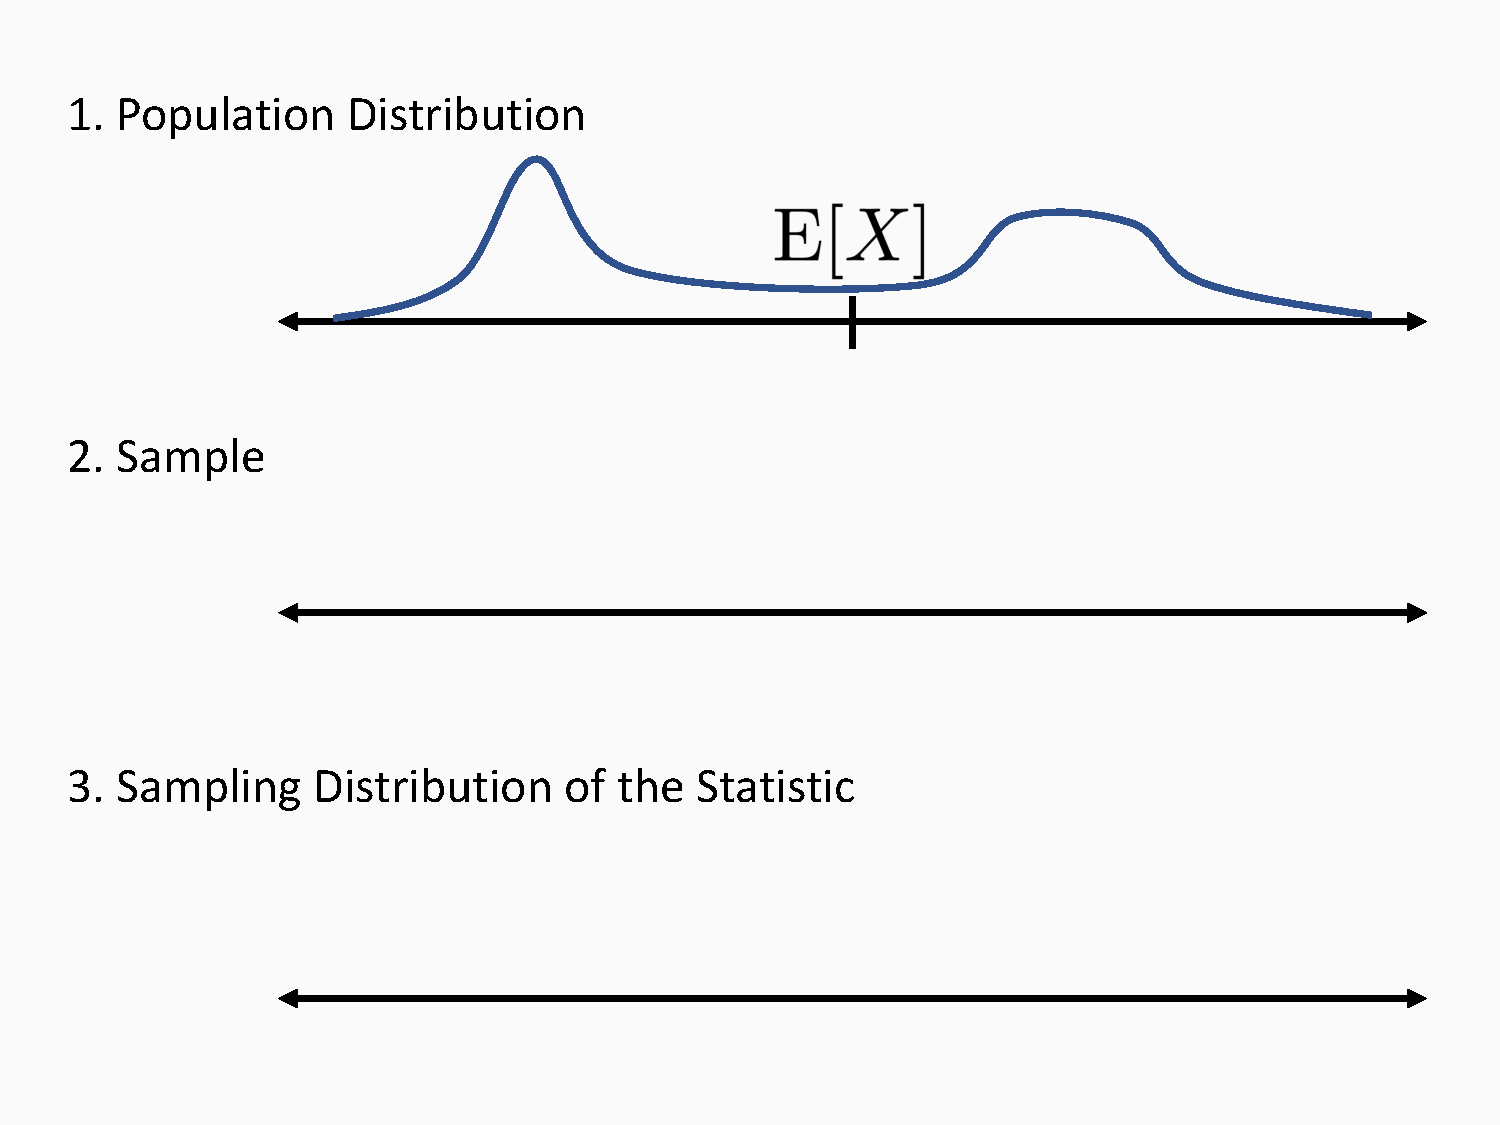
\includegraphics[width = \textwidth]{./images/mean_estimator}

\note[item]{Here's a picture to clarify how the model works.}
\note[item]{There are three important objects to keep in mind.}
\note[item]{First, we have the population distribution, we don't know what it is, but it's fixed, and it has a fixed population mean.}
\note[item]{What happens when we run the model?  nature reaches in and chooses datapoints.  I'll make a sample.}
\note[item]{From this sample, we compute the sample mean.  Does it equal the population mean?  of course not!  well, in some cases we could get lucky, but generally no.}
\note[item]{what kind of object is the sample mean? it's a random variable.  if you could rewind time, we'd get a different mean. }
\note[item]{I'm not saying we can get two means, this is just a thought experiment.}
\note[item]{because the sample mean is a random variable, it has a sampling distribution.  I'll draw it here.}
\note[item]{There are two different distributions!  don't forget that, the population dist is not the same as the sampling distribution of the statistic.}
\end{frame}

\begin{frame}
  \frametitle{Evaluating the Sample Mean as an Estimator}
  \note[item]{Once you start thinking about the sample mean as an estimator, the next step is to think about whether it's a good estimator. Are there any better estimators?}
  \note[item]{What are the properties that we want our estimators to have?}
  \note[item]{Let's start in this segment with these two. <read>}
  First Questions:
  
  \begin{enumerate}
  \item Is the sample mean biased?
  \item How efficient is the sample mean?
  \end{enumerate}
\end{frame}




\begin{frame}[t]
  \frametitle{Unbiasedness of the Sample Mean}
  \begin{block}{Theorem: The Sample Mean is Unbiased}
    For IID random variables, $X_1,..X_n$, the sample mean $\overline{X}$ is an unbiased estimator for the population mean $\E[X]$.
    \end{block}
\note[item]{$E[\overline{X}] =  E[\frac{1}{n} (X_1 + X_2 +...+X_n)  ]$}
\note[item]{$= \frac{1}{n} (E[X_1] + ... + E[X_n]) = E[X]$}
\end{frame}


\begin{frame}[t]
  \frametitle{Efficiency of the Sample Mean}
  \begin{block}{Theorem: Sampling Variance of the Sample Mean}
    For IID random variables, $X_1,..X_n$, with population variance, $\V[X]$, the variance of the sample mean is
     \[
        \V\big[\overline{X}\big] = \frac{\V[X]}{n}
      \]
    \end{block}
    \note[item]{  $      \V\big[\overline{X}\big]  = \V[ \frac{1}{n} (X_1 + X_2 +...+X_n)] $}
    \note[item]{$= \frac{1}{n^2} ( \V[X_1] + ... + \V[X_n] ) = \frac{\V[X] }{n} $}
    \note[item]{Is this a good variance?  It really depends on the population distribution.  Depending on what the population looks like, there could be more efficient estimators.  But at least the dependency on $n$ is good.  we know that if we get enough data, we can get a low variance estimate.}
    \note[item]{Soon, we'll see that we can get a guarantee that the sample mean is actually close to the target.}
\end{frame}

\begin{frame}
  \frametitle{Learnosity: Sampling Variance of the Sample Mean}
  \textbf{Note: This is a learnosity activity, just placing it here
    for organization.}

  \begin{itemize}
  \item If you increase the sample size, does the sampling variance of
    the sample mean increase, decrease, or stay the same?
  \item At what rate does this change? (Options include faster than
    the data, at the same rate at the data, slower than the data.)
    \note[item]{One is an increase, one a decrease, so not sure how to map
      $1/n$ to these options}
  \item If you increase the sample size, does the population variance,
    $\V[X]$, change? (Hint: It is a population parameter.)
  \end{itemize}
\end{frame}

% \section{Convergence and Chebyshev}

% \begin{frame}
%   \frametitle{Chebyshev's Implications}
%   \note[item]{Chebyshev's inequality isn't difficult to prove, but we
%     want to cut to the chase rather than having your read it.}
%   \begin{itemize}
%   \item Pick some small $\epsilon$ and think about the window from,
%     $E[X] \pm \epsilon$
%   \item Then, the probability the sample mean is outside the window is less than:
%   \end{itemize}
%   \begin{align*}
%     Pr\big[\big|\overline{X} - E[X]\big| \geq \epsilon \big]
%     &\leq \frac{V\big[\overline{X}\big]}{\epsilon^{2}} \\
%     & \leq \frac{V[X]}{\epsilon^{2}n} 
%   \end{align*}
%   \note[item]{\paul{maybe add a take-away: If we know variance is
%       small, we can turn that into a statement saying that values far
%       from the mean are unlikely.}} 
%   \note[item]{\paul{maybe add a picture to show the Real number line
%       with the window around the mean}} 
% \end{frame}

% \begin{frame}
%   \frametitle{Chebyshev's Implications} 
%   \textbf{Note: This is a handwriting slide to draw what Chebyshev's
%     says}

%   \note[item]{With any arbitrary function -- makes a wavy function --
%     how far a sample average is from $E[X]$ is still well-behaved.}
%   \note[item]{In paricular, the larger is $V[X]$, the larger this
%     probability can be.}
%   \note[item]{The larger is the draw, $n$, the smaller this
%     probability will tend to be.}
%   \note[item]{Suppose that $V[X] = 100$, and $E[X] = 6$, and $n=100$.}
%   \note[item]{Set $\epsilon$ initially to be 2}
%   \note[item]{\paul{Love it!}}
% \end{frame}

% \section{Chebyshev and Convergence in Probability}

% \begin{frame}
%   \frametitle{Chebyshev and Convergence in Probability}
%   \textbf{I think that we should cut this to get to WLLN.} 
%   \paul{I'm thinking that consistency is more important than
%     Chebyshev.  How about  
  
%   1. breezing through chebyshev with just one slide, no drawing. then 
  
%   2. a slide to define convergence in probability with the equation.
  
%   then 3. a third slide to do some drawing to understand what
%   convergence in probability means: 
  
%   choose an $\epsilon$ and draw a window $[c-\epsilon,
%   c+\epsilon]$. at first, there's some probability your statistic is
%   in the window, say 50\%.  that's not good enough.  but you know you
%   can crank n up, and this approaches 1. say you crank n up until the
%   probability is 99\%.  Then you want to be even closer.  so divide
%   $n$ by two to make the window even smaller.  now you crank n up some
%   more, util the probability is 99\% again.  this is a probability
%   limit - you can be as confident you want for a window that's as
%   small as you want (not zero).  
  
%   4. finally, voila!  notice that the equation in chebyshev is almost
%   suited for the definition of convergence in probability - look at
%   the book for the proof. 
%   }
% \end{frame}

\section{Consistency and the Continuous Mapping Theorem}


\begin{frame}
  \frametitle{Consistency}
  
 
\begin{center}
\textit{"If you can't get it right as $n$ goes to infinity, you shouldn't be in this business."}
\end{center}
\begin{flushright}
\vspace{-.3cm} - Clive W.J. Granger
\end{flushright}
\vspace{.5cm}

  \note[item]{It's no exaggeration to say that consistency is the most important property that an estimator can have.}
  \note[item]{So what exactly does it mean?}
  \note[item]{A quote from the Nobel-prize winning economist Clive Granger.}
  \note[item]{We want to be correct as the sample size gets bigger and bigger - how can we write that into a mathematical property?}
  \note[item]{it's not obvious for at least two reasons.}
  \note[item]{First, different estimators can converge at different rates.  it may take $n=10$ or $n=10M$ to be close, and we need a guaratee that works for both, so have to abstract away from specific numbers.}
  \note[item]{Second, there's no deterministic guarantee.  There's no law of physics that prevents a coin from landing heads over and over forever.  all we can say is that the probability of that gets smaller and smaller as the number of flips increases.}
  
How can we formalize "right as $n$ goes to infinity?"
  \begin{itemize}
\item Estimators may converge at different rates.
\item Deterministic guarantees are not possible.
\end{itemize}

\end{frame}

%\begin{frame}
%  \frametitle{An Example of Convergence}
%  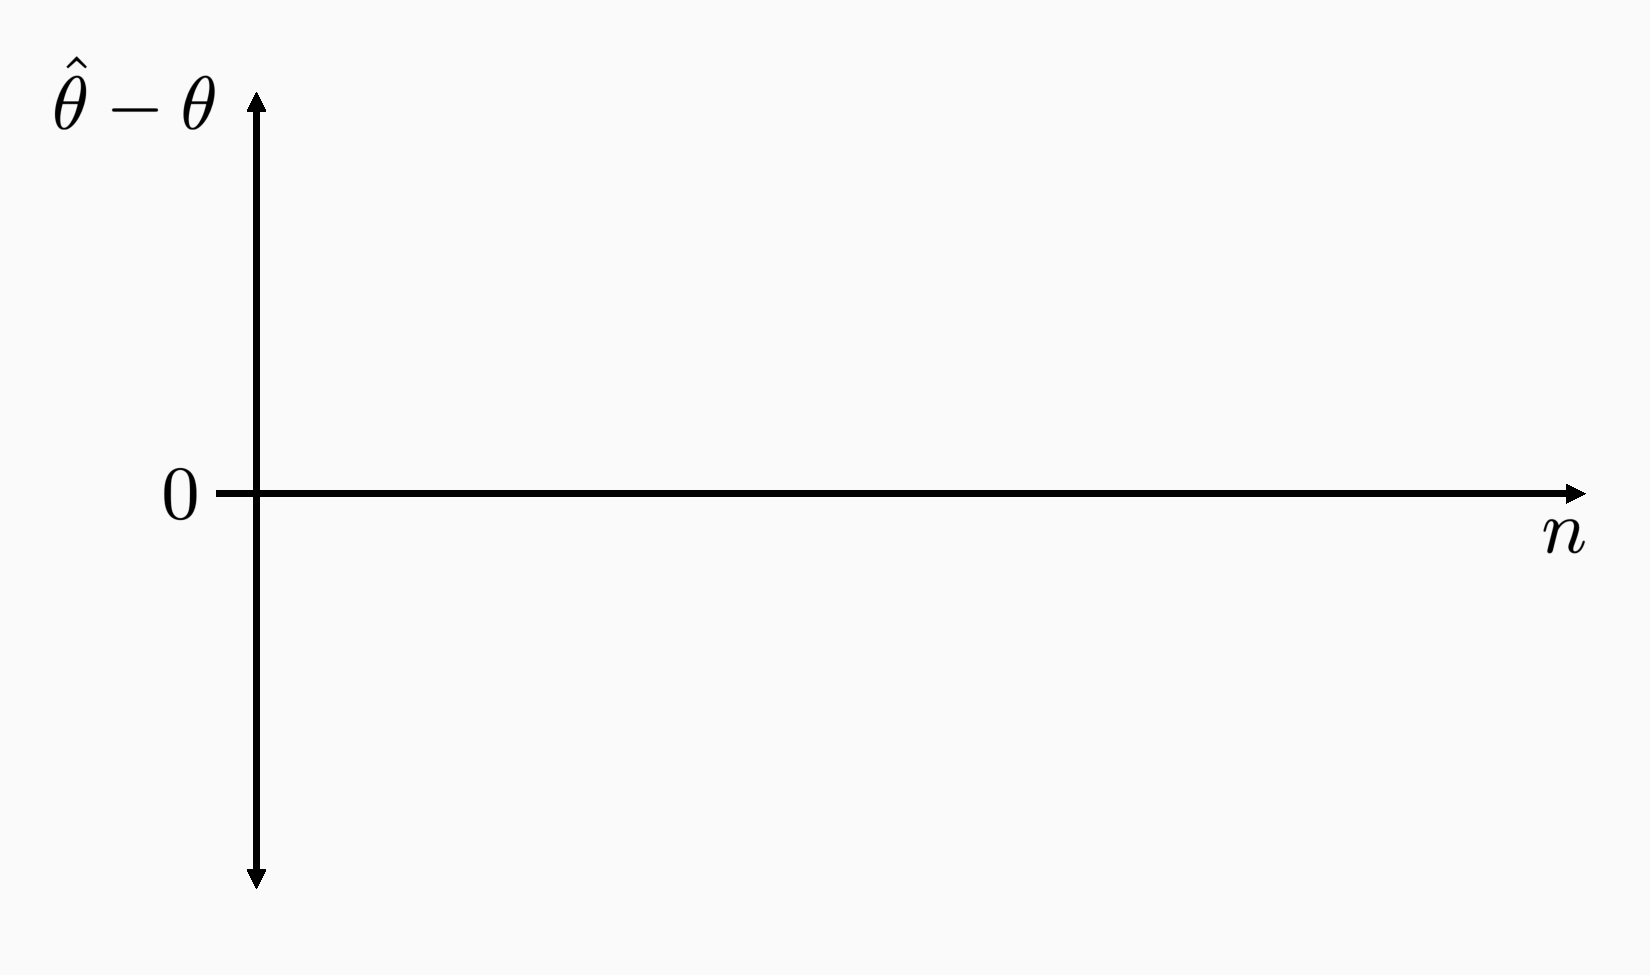
\includegraphics[width= \textwidth]{./images/convergence_axes}
%  \note[item]{First, here's a picture of what convergence might look like}
%  \note[item]{Imagine that this is the sample mean, we're talking about.}
%  \note[item]{On the y-axis, we have the estimator minus the true parameter.}
%  \note[item]{Say I start with a sample of just 1.  that value might be really far from the population mean}
%  \note[item]{one by one, I draw a new data point and add it to my sample, and I recompute the mean. what happens?}
%  \note[item]{Of course the mean jumps up and down, but what we expect is that it should settle down.}
%  \note[item]{again, there's no deterministic law that says that it has to, it's just what we expect with high probability.}
%\end{frame}


\begin{frame}
  \frametitle{Intuition for Convergence in Probability}
\begin{itemize}
\item Let $T_{(1)}$ be the statistic with 1 datapoint.
\item Let $T_{(2)}$ be the statistic with 2 datapoints.
\item Let $T_{(3)}$ be the statistic with 3 datapoints.
\end{itemize}
\hspace{1.6cm} \vdots

  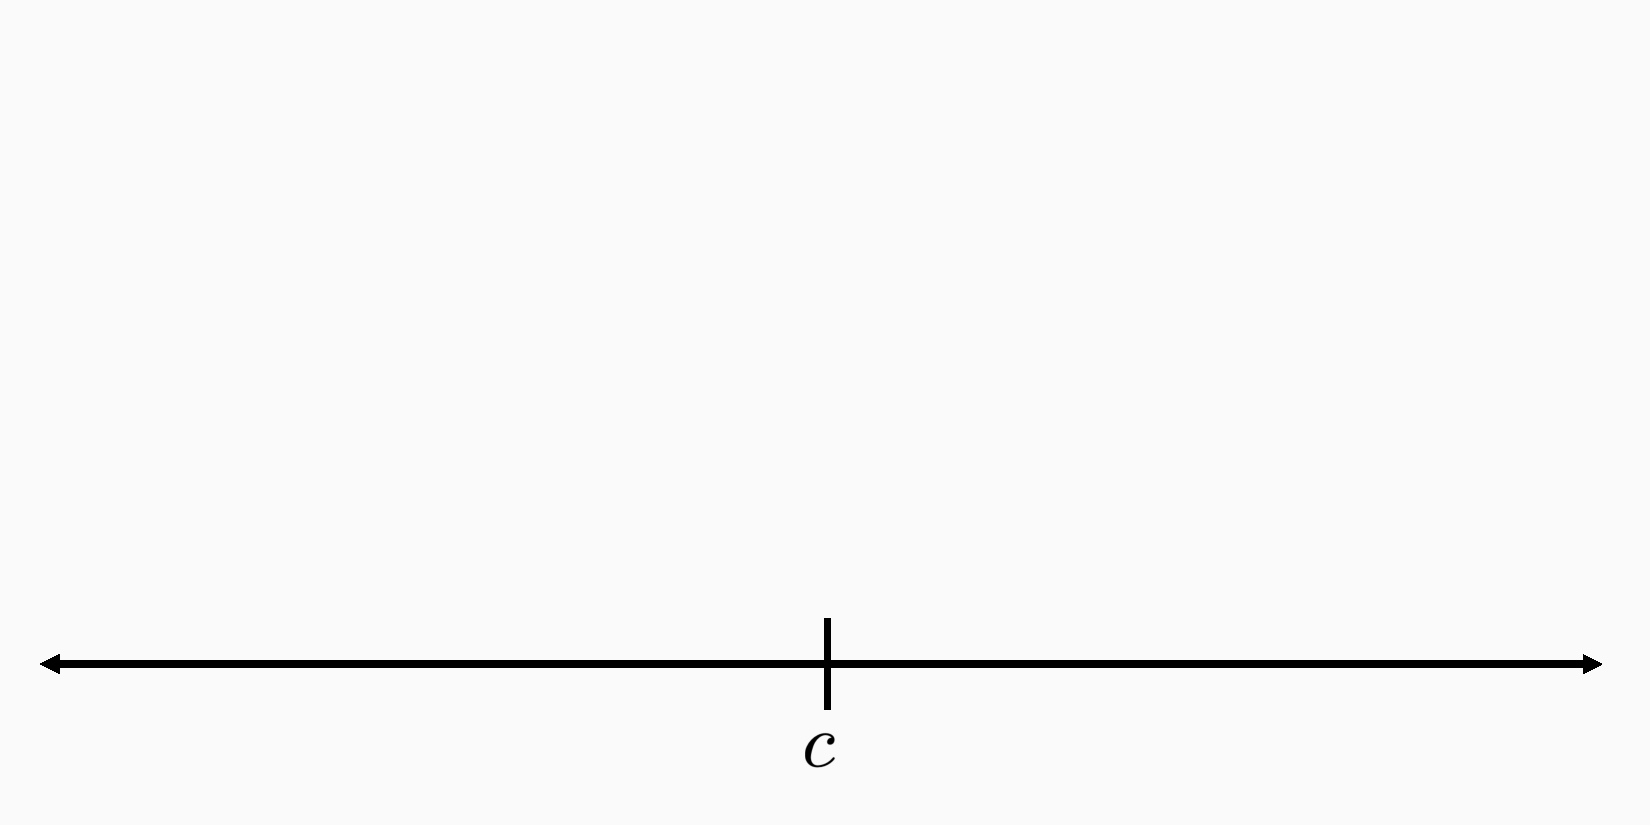
\includegraphics[width= \textwidth]{./images/convergence_window}
\note[item]{Here's a stylize story to motivate the definition of consistency.}
\note[item]{Let's start with a sequence of random variables <read>}
\note[item]{Let $c$ be the target we're aiming for.}
\note[item]{You tell me you want to converge on the target.  So I say, well give me some parameters, give me a window around the target that is acceptable.  also, 100\% guarantees don't exist, so give me a probability you can live with.}
\note[item]{I guarantee, that eventually in this sequence, there is a T that is in that window with 90\% probability}
\note[item]{Is the guarantee not strong enough? feel free to increase it:  let's say 99\%.  I can crank n up more, and make sure the probability is 99\%.}
\note[item]{Is the window actually too wide? make it narrower!...}
\end{frame}



%
%
%\begin{frame}[t]
%  \frametitle{Consistency and Convergence}
%  Can we use the sample mean, $\overline{X}$, to estimate the
%  population expected value?
%  \note[item]{Can we use $\overline{X}$ to estimate $E[X]$? \textbf{We demand some guarantees!}}
%  \note[]{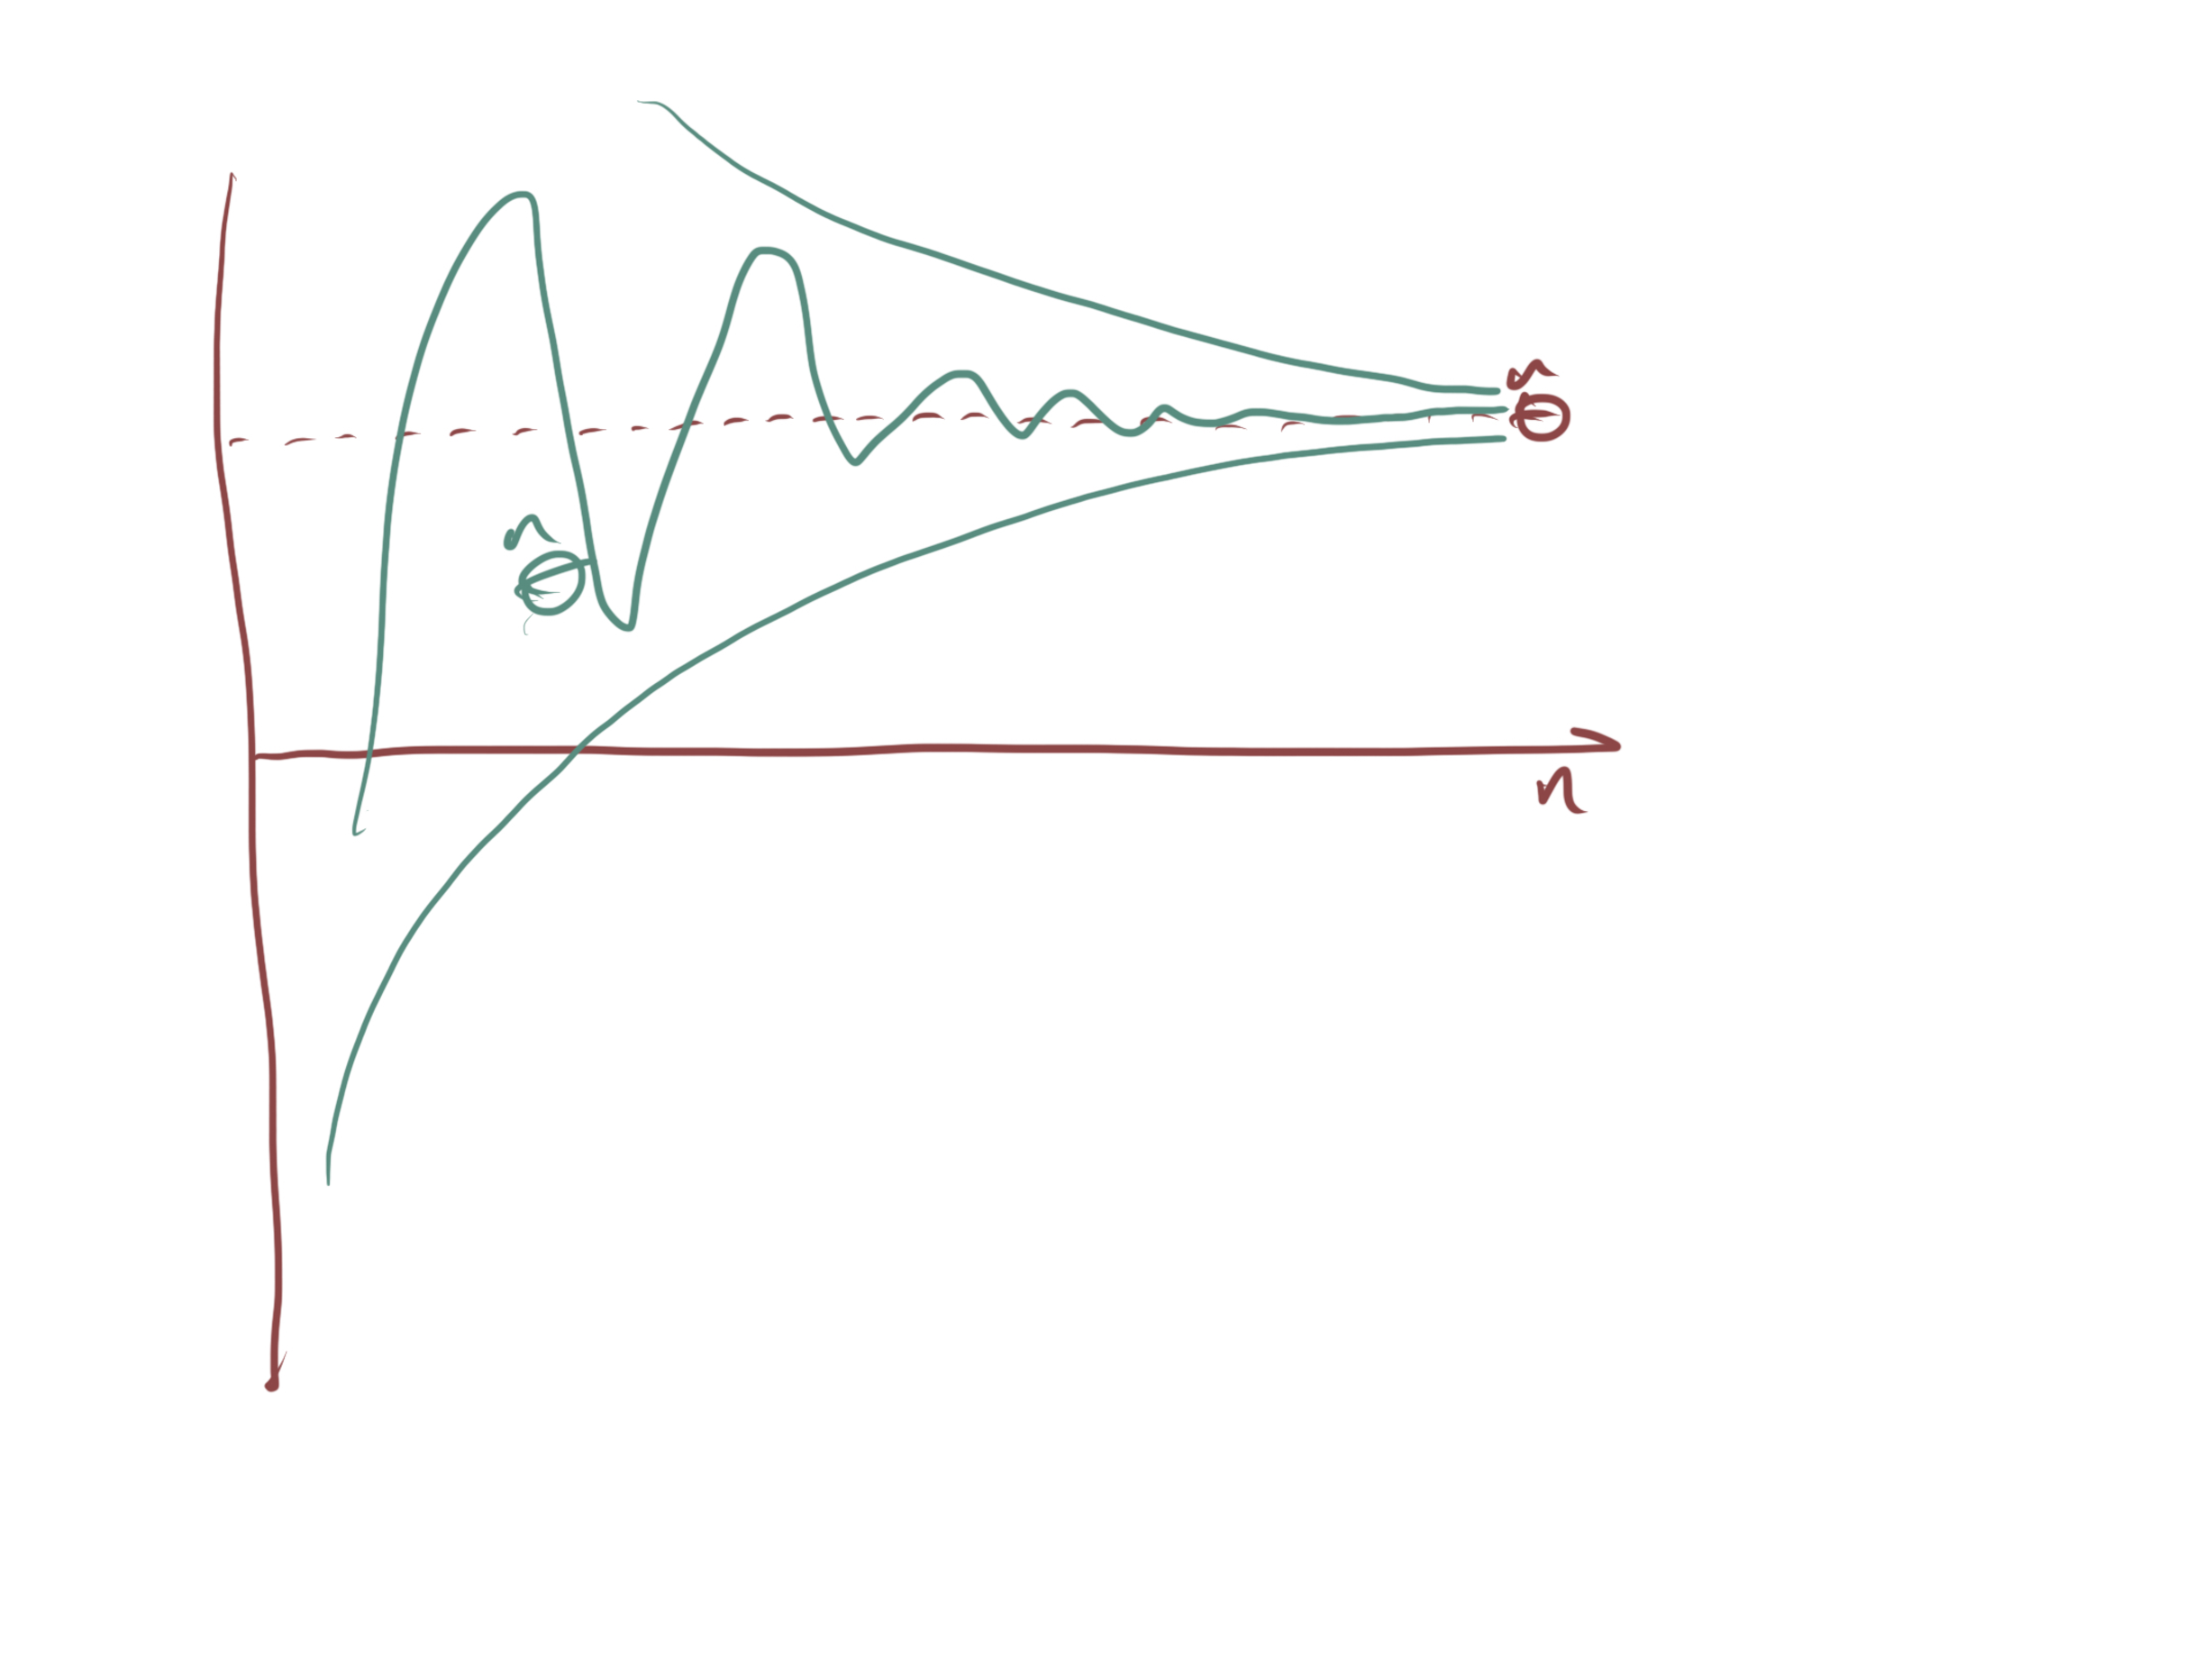
\includegraphics[width=.25\linewidth]{./images/consistency}}
%  \begin{itemize}
%  \item A minimum requirement for most \textit{estimators} is that as $n\to\infty$, $\hat{\theta}$
%    gets \textit{closer} to $\theta$.    
%    \note[item]{Chebyshev, together with a classic, the squeeze theorem, gives us this guarantee!}
%  \end{itemize}
%  $$
%  Pr\big[\big|\overline{X} - \E[X]\big| \geq \epsilon \big] \leq \frac{\V[X]}{\epsilon^{2}n} 
%  $$
%  \note[item]{Draw this. Note that $V[X]$ is a population
%    characteristic that just \textit{is}. And, we're choosing
%    $\epsilon$, so that is also set. Then, we can see that as $n$
%    increases, the $P(|\overline{X} - E[X]| > \epsilon) \to 0$.}
%  \note[item]{Flipping this just a little bit, we would say that
%    $\overline{X}\overset{p}{\to}E[X]$.}    
%\end{frame}

\begin{frame}
  \frametitle{Convergence in Probability}

  \begin{block}{Definition: Convergence in Probability} 
    Let $( T_{(1)}, T_{(2)}, T_{(3)},...) $ be a sequence of random variables and let $c\in \R$. $T_{(n)}$  \textit{converges in probability} to $c$ if for all $\epsilon > 0$, 
    $$\lim_{n \rightarrow \infty} P\Big[ T_{(n)}  \in (c-\epsilon, c+\epsilon) \Big] = 1$$
    We write this as $T_{(n)} \overset{p}{\rightarrow} c$.
      \end{block} 
      
      \begin{itemize}
\item An estimator $\hat \theta$ is \textit{consistent} for $\theta$, if $\hat \theta \overset{p}{\rightarrow} \theta$.
\end{itemize}

\end{frame}

\begin{frame}
  \frametitle{Continuous Mapping Intuition}
  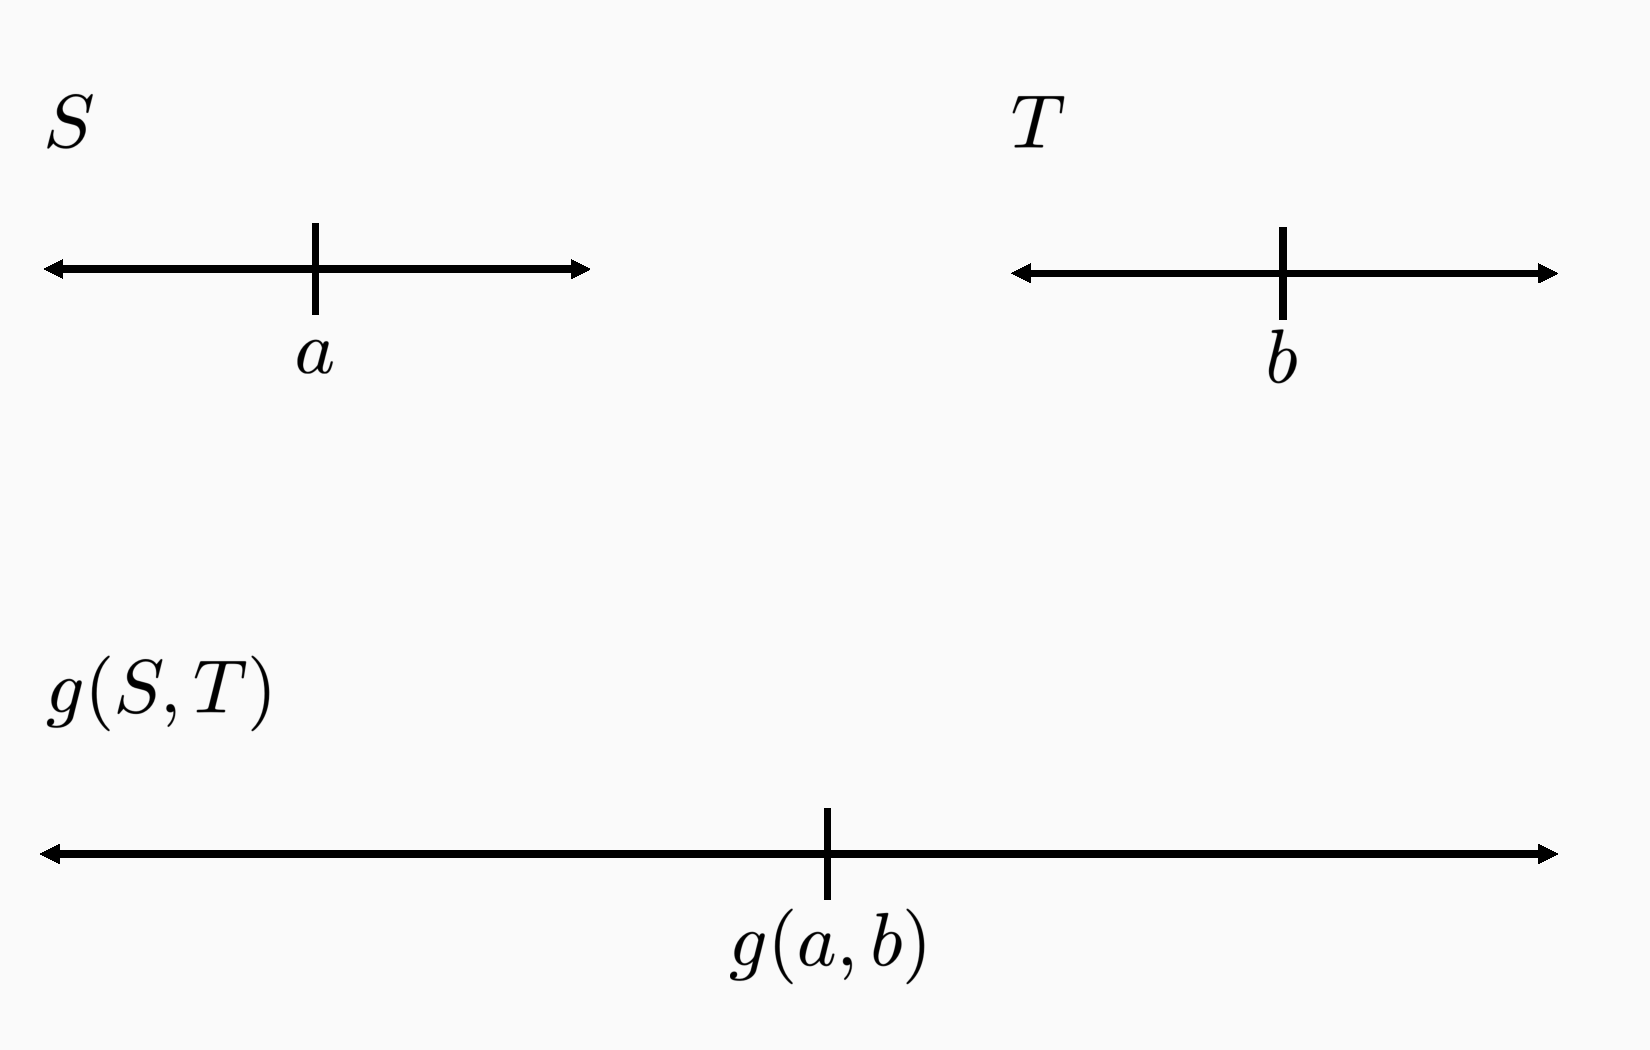
\includegraphics[width= \textwidth]{./images/cmt}
  
  \note[item]{Consistency is really important.  We're going to design a lot of estimators and we'll want to prove that they are consistent.}
  \note[item]{There are different strategies you can use to prove that estimators are consistent.  The book likes to use a very powerful result about the plug in principle, but you have to know a lot more math to apply it rigorously.}
  \note[item]{We prefer to use a famous theorem called the continuous mapping theorem.  It allows you to prove convergence in probability when you combine estimators together. }
  \note[item]{Here's a picture to show what we mean.  we have two estimators S and T that each converge to some target.  We have a function g that takes a,b to this point.  As long as g is consistent, it turns out that g(S,T) is also consistent.}
\end{frame}


\begin{frame}[t]
 % \frametitle{The Continuous Mapping Theorem}

  \begin{block}{The Continuous Mapping Theorem} 
    Let $( S_{(1)}, S_{(2)}, S_{(3)},...) $ and $( T_{(1)}, T_{(2)}, T_{(3)},...) $ be two sequences of random variables.  Let $g: \R^2 \rightarrow \R$ be a continuous function.  If $S_{(n)} \overset{p}{\rightarrow} a \in \R$ and $T_{(n)} \overset{p}{\rightarrow} b \in \R$, then $g(S_{(n)}, T_{(n)})  \overset{p}{\rightarrow} g(a,b)$
      \end{block} 
      
      \note[item]{Given $\epsilon > 0$, let $W = (g(a,b) - \epsilon, g(a,b) + \epsilon)$.}
      \note[item]{Want $lim_{n\rightarrow \infty} P( g(S_n,T_n) \in W) \rightarrow 1)$}
      
 \note[item]{Equivalent to:  given probability $\alpha >0$ $\exists n$ such that $P(g(S_n,T_n) \notin W) < \alpha$.}
      \note[item]{By cont. of $g$, $\exists \lambda > 0$ such that if $S_{(n)} \in I_a = (a-\lambda, a+\lambda)$ and $T_{(n)} \in I_b (b-\lambda, b+\lambda)$ $g(S_{(n)}, T_{(n)}) \in W$}
      \note[item]{by convergence of S and T, $\exists n_1, n_2$ such that $P(S_{(n_1)} \notin I_a) < \alpha/2$ and $P(T_{(n_2)} \notin I_b <\alpha/2$}
      \note[item]{let $n = max(n_1,n_2)$, then $P(S_{(n_1)} \notin I_a \cup T_{(n_2)} \notin I_b) \leq \alpha/2 + \alpha/2 = \alpha$. }
      \note[item]{ This implies  $P(g(S_{(n)}, T_{(n)}) \in W) > \alpha$}
      
\end{frame}


\section{Reading: Weak Law of Large Numbers}

\begin{frame}
  \frametitle{Reading: Weak Law of Large Numbers }
  Read page 100, beginning at theorem 3.2.8, through the end of page
  102. 
\end{frame}

\section{Weak Law of Large Numbers}

\begin{frame}
  \frametitle{The Weak Law of Large Numbers}
\note[item]{We have all the pieces in place to present one of the most classic results in statistics.}
\note[item]{The WLLN states that as sample size increases, the sample mean converges in probability to the population mean.}
\note[item]{Or much more simply, the sample mean is consistent.}  

  \begin{block}{Theorem: The Weak Law of Large Numbers}
  Let $(X_1,X_2,X_3,...)$ be a sequence of i.i.d. random variables with finite variance.  Let $\overline{X}_{(n)} = \frac{1}{n}\sum_{i=1}^n X_i$.  Then
  $$ \overline{X}_{(n)} \overset{p}{\rightarrow} \E[X]$$
  \end{block}
  
  \begin{itemize}
\item \textbf{Equivalently:} The sample mean is \textit{consistent} for the population mean.
\end{itemize}

\end{frame}


\begin{frame}
  \frametitle{Consequences of WLLN}
  \note[item]{What do we take away from the WLLN?}
  \note[item]{First, we learned that the sample mean is great.  On top of being unbiased, we also have consistency.}
  \note[item]{Whatever the variable is: wavelengths of cosmic rays, or how cranky people in Berkeley are.  You never know the true population mean, but if you crank up n enough, you'll can be accurate to any level.}
  \note[item]{Now, honestly, you already knew the sample mean was great.  you don't need more reasons to use the mean.  And we can write down more precise statements about the convergence of the sample mean.  So why is the WLLN so important?}
  \note[item]{But is a second reason WLLN is important.  it is a building block we can use to study other estimators.}
  \textbf{The sample mean is consistent.} 
  \begin{itemize}
  \item The error converges in probability to zero.
  \item The sample mean is accurate, as long as we can make $n$ large enough.
  \end{itemize}
  \textbf{As a building block to study other estimators.}
  \begin{itemize}
  \item Combine WLLN with Continuous Mapping Theorem.
  \end{itemize}
\end{frame}

\begin{frame}[t]
  \frametitle{Applying the WLLN}
  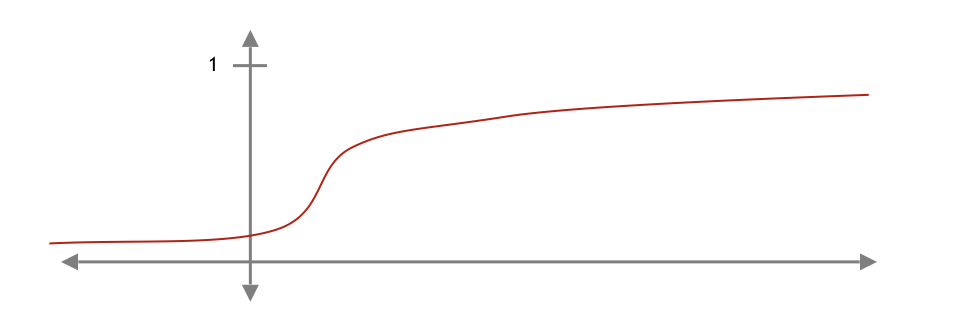
\includegraphics[width = \textwidth]{./images/cdf2}

  \textbf{Objective:} Estimate the cdf $F$ at a point $x$.
  
\note[item]{F(x) = P(X < x)}
  
  \textbf{Idea:} Use empirical cdf
  
  \note[item]{$T_{(n)}(x) = \frac{1}{n} \sum I(X_i \leq x)$}
  
  \note[item]{$T(x) \overset{p}{\rightarrow} \E[ I(X \leq x) ] = P(X \leq x) = F(x)$}

  \note[item]{So we can consistently estimate the CDF at any point.}
  \note[item]{There are stronger convergence results for the cdf, so we don't use this version too much} 
  \note[item]{But this is an example of how WLLN can help us with other estimators.  we'll use it again in the future.}
\end{frame}

\section{Proof of the Weak Law of Large Numbers}

\begin{frame}[t]
  \frametitle{Proof of the Weak Law of Large Numbers}
  Given random variable $X$ and $\epsilon > 0$.
\end{frame}


\begin{frame}[t]
  \frametitle{Proof of the Weak Law of Large Numbers}
  Given random variable $X$ and $\epsilon > 0$.
  
  Let $D = | \bar X - \E[X] |$
  
  $\V[\bar X] = \E[D^2] = \V[X]/n$
  
  $\V[\bar X] = \E[D^2] = \E[D^2 | D < \epsilon] P(D < \epsilon) + \E[D^2 | D \geq \epsilon]P(D \geq \epsilon)$
  
  $\geq 0 + \epsilon^2 P(D \geq \epsilon)$
  
  $P(D \geq \epsilon) \leq \frac{\V[X]}{ \epsilon^2 n} \overset{p}{\rightarrow} 0$
  
  \note[item]{The key to this proof is we have to get from a small variance to a statement about deviations.}
  \note[item]{Why can't we be outside this window?  Let's draw the probability distribution.}
  \note[item]{The point is that if there's some probability outside the window, that represents deviations that are large, and that has the effect of keeping variance up. that can't happen.}
\end{frame}

\section{Simulating the WLLN}

\begin{frame}
  \textbf{Note: This is a learnosity activity, we're just including it
    here for organization.}
  Students will work through the notebook called \texttt{WLLN.Rmd.}
\end{frame}


 
\section{Reading: Estimating Population Variance}

\begin{frame}
  \frametitle{Reading: Estimating Population Variance}
  \note[item]{\textbf{Note: This is a READING CALL, just placing it here
      for organization.}}
  \begin{itemize}
  \item Read pages 105–108, stopping before the beginning of the
    next section. 
  \item You are going to use \textit{the plug-in principle}, which is
    a general approach for designing estimators in a sample. 
    \note[item]{Write down what we want for the population, use a
      sample to estimate it, check the characteristics of the
      estimator using math.}
  \end{itemize} 
\end{frame}
 
\section{Estimating Population Variance}

\begin{frame}
  \frametitle{Why Estimate Variance?}
  
  \note[item]{So far, we've talked about estimating the population mean.}
  \note[item]{The mean is really important, but there are other quantities that we might want to estimate.}
  \note[item]{Let's consider the variance - usually the second-most important feature you can learn.}
  \note[item]{If you estimate mean coffee intake, that's is helpful, but just one number, nothing about the shape of the distribution.}
  \note[item]{IF you also know variance, you start to have at least some information about shape.  That can really improve your understanding.}
  
   \center 
\includegraphics[width = .9\textwidth]{./images/coffee}

\begin{itemize}
\item How much coffee do students drink on average?
\item How much does coffee intake differ from student to student?
\end{itemize}
 
\end{frame}



\begin{frame}[t]
  \frametitle{Applying the Plug-In Principle}
Population Variance: $ \V[X] = \E[X^{2}] - \E[X]^2 $
\vspace{1cm}
  
  \begin{block}{The Plug-In Variance Estimator}
  Given a sample $\bs X = (X_1,X_2,...,X_n)$, the \textit{plug-in variance estimator} is,
    \begin{align*}
\tilde{\V}(\bs X) &= \overline{X^{2}} - \overline{X}^{2}
    \end{align*} 
  \end{block}
  \note[item]{How do we come up with an estimator for variance?}
  \note[item]{We use what we call the plug-in principle.  All that means is that we just replace population quantities with sample analogues.}
  \note[item]{In this case, we can write the variance as the difference of two expectations.}
  \note[item]{We just replace each expectation with a sample mean.}
\end{frame}



\begin{frame}[t]
  \frametitle{Consistency of the Plug-In Estimator}
  
  \begin{block}{Theorem: Consistency of the Plug-In Variance Estimator}
  Let $(X_1,X_2,X_3,...)$ be a sequence of i.i.d. random variables with finite variance $\V[X]$.  Then $\tilde{\V}(\bs X)=\overline{X^{2}} - \overline{X}^{2}$ is consistent for $\V[X]$.
  \end{block}
  \note[item]{Proof: $\overline{X} \overset{p}{\rightarrow} \E[X]$}
\note[item]{$\overline{X^2} \overset{p}{\rightarrow} \E[X^2]$}
\note[item]{Let $g:\R^2 \rightarrow \R, g(a,b) = a -b^2$.  g is continuous}
\note[item]{$g(\overline{X^2}, \overline{X}  ) = \tilde{\V}(\bs X)  $}
\note[item]{CMT $\implies g(\overline{X^2}, \overline{X}  )  \overset{p}{\rightarrow} g(\E[X^2],\E[X]) = \V[X] $}
\end{frame}

\begin{frame}[t]
  \frametitle{Bias of the Plug-In Variance Estimator}
  \note[item]{What about bias?  Unfortunately, the plug-in estimator is biased.  That's pretty common, the plug-in principle often gives us consistent estimators, but doesn't help with bias.}
  \note[item]{You can compute the expectation of the estimator, and you can see that it's almost what you want.}
  \note[item]{There's just an extra factor of $(n-1)/n$.  You can read the proof in the book.  We aren't including it because we don't think it adds much intuition.  }
  \note[item]{If you think about it, if we knew the true population mean, we could measure deviations from it to get an unbiased estimator.  But we have the sample mean, and the sample mean gets pulled towards where the most data is, pushing the estimate down.}

  
    Let $(X_1,X_2,X_3,...)$ be a sequence of i.i.d. random variables with finite variance $\V[X]$.  Then
  $$\E[\tilde{\V}(\bs X)] = \frac{n-1}{n} \V[X]$$


\end{frame}


\begin{frame}
  \frametitle{A Better Variance Estimator}
  
    \begin{block}{The Unbiased Variance Estimator}
  Given a sample $\bs X = (X_1,X_2,...,X_n)$, the \textit{unbiased sample variance estimator} is,
    \begin{align*}
\hat{\V}(\bs X) &= \frac{n}{n-1} \Big( \overline{X^{2}} - \overline{X}^{2} \Big)
    \end{align*} 
\end{block}
\note[item]{So the plug-in estimator is biased, but we know exactly what the bias is so we can fix it.}
  \note[item]{We just adjust it by adding a correction factor.  It's called a degrees of freedom correction.}
  \note[item]{This makes the estimator unbiased, and it's still consistent, because this fraction goes to 1.}
  \note[item]{This estimator has really good properties, and it's the standard formula you should remember. }
\end{frame}



\section{Standard Errors}

\begin{frame}[standout]
\note[item]{We've been talking about ways to generate a point estimate for a parameter.}
\note[item]{But the point estimate is really only half the story.}
\note[item]{That's because the point estimate is not the same as the true parameter.}
\note[item]{If all you have is the point estimate, and no other way to judge how far off it might be, it may not be very valuable at all.}
\note[item]{If you're just messing around with data for fun, you may not care, but when the stakes get high, you realize you really need a way to capture that uncertainty.}
\center Point Estimate $\Leftrightarrow$ Uncertainty
\end{frame}


\begin{frame}
  \frametitle{Importance of Uncertainty}
     \center 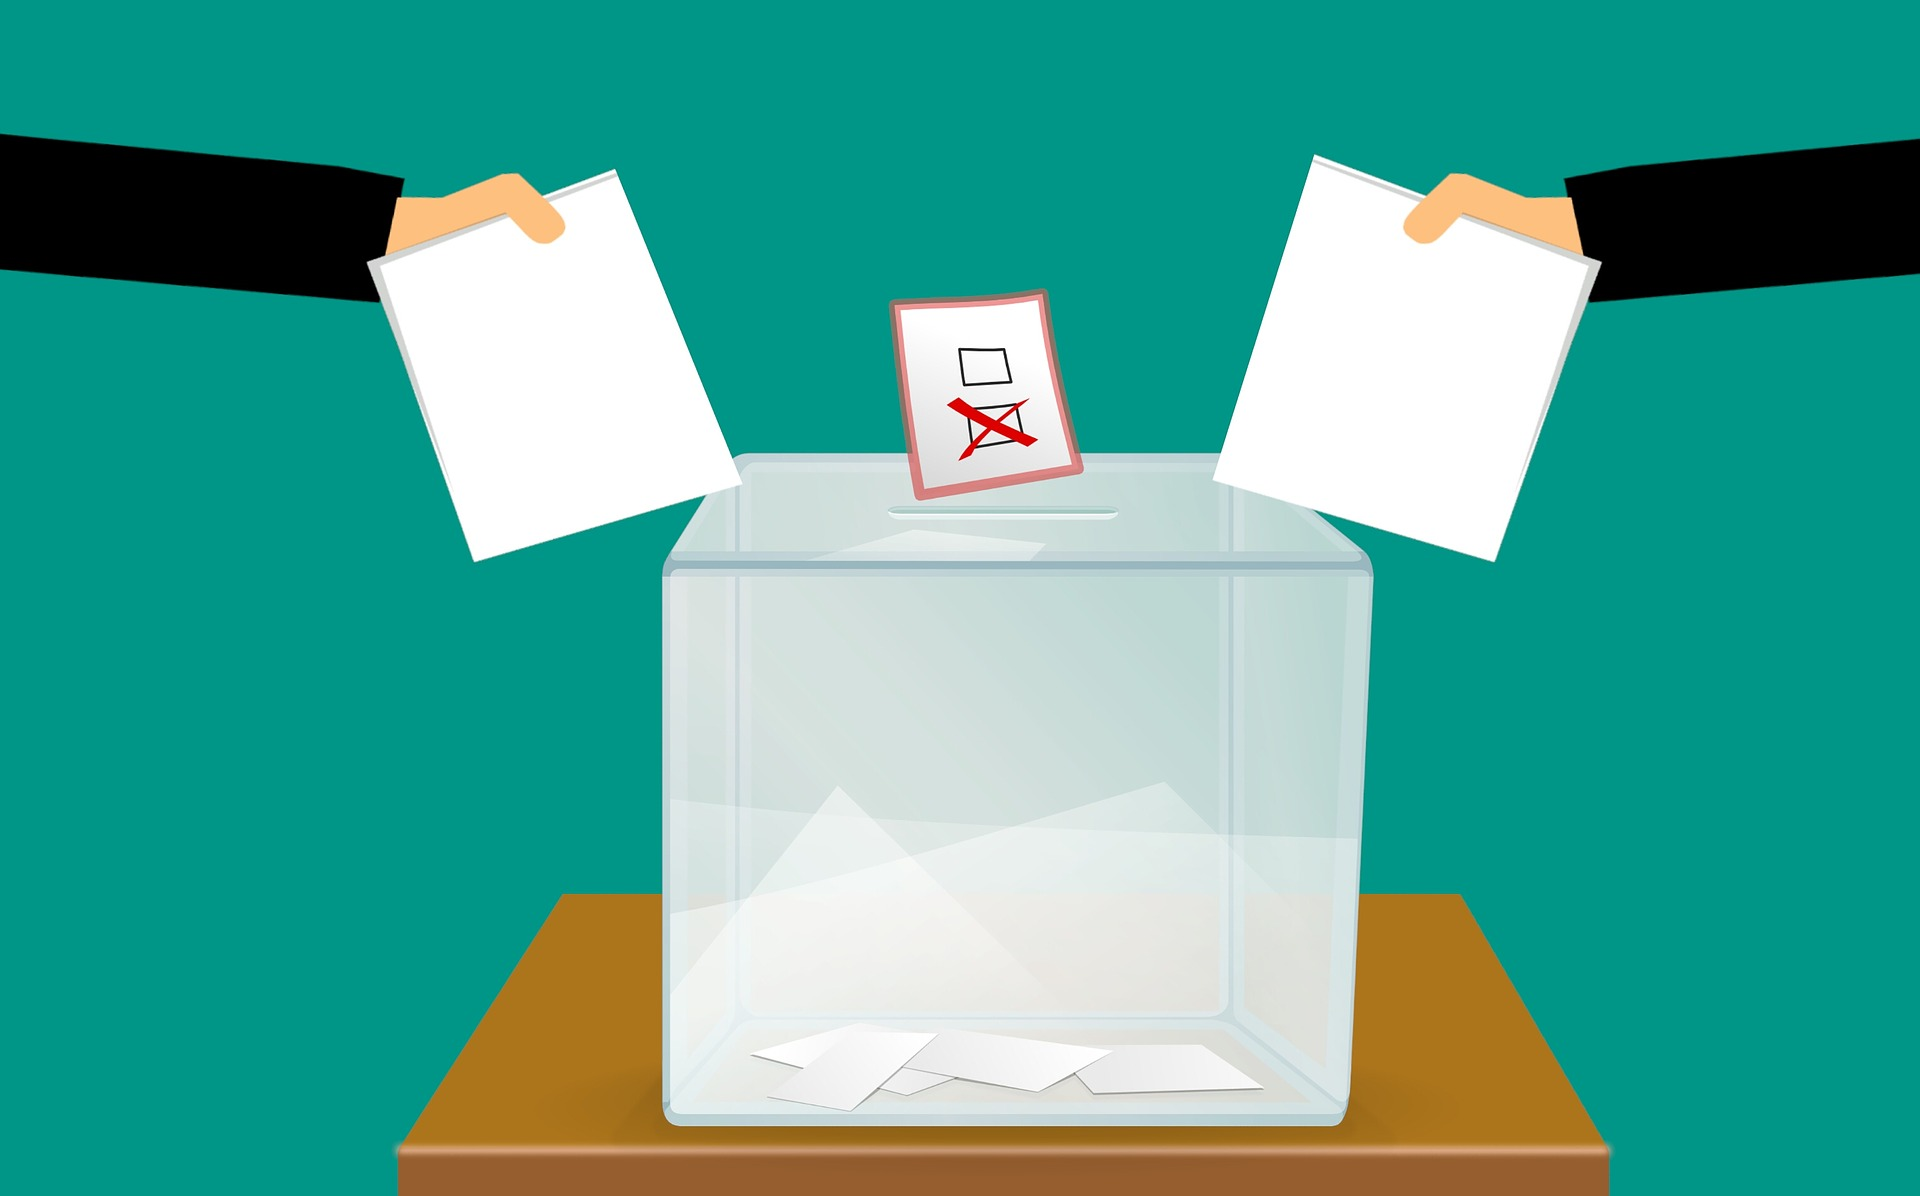
\includegraphics[width = \textwidth]{./images/vote}

\textbf{Estimate:} Our candidate has 52\% support.
\end{frame}


\begin{frame}
  \frametitle{Importance of Uncertainty}
       \center 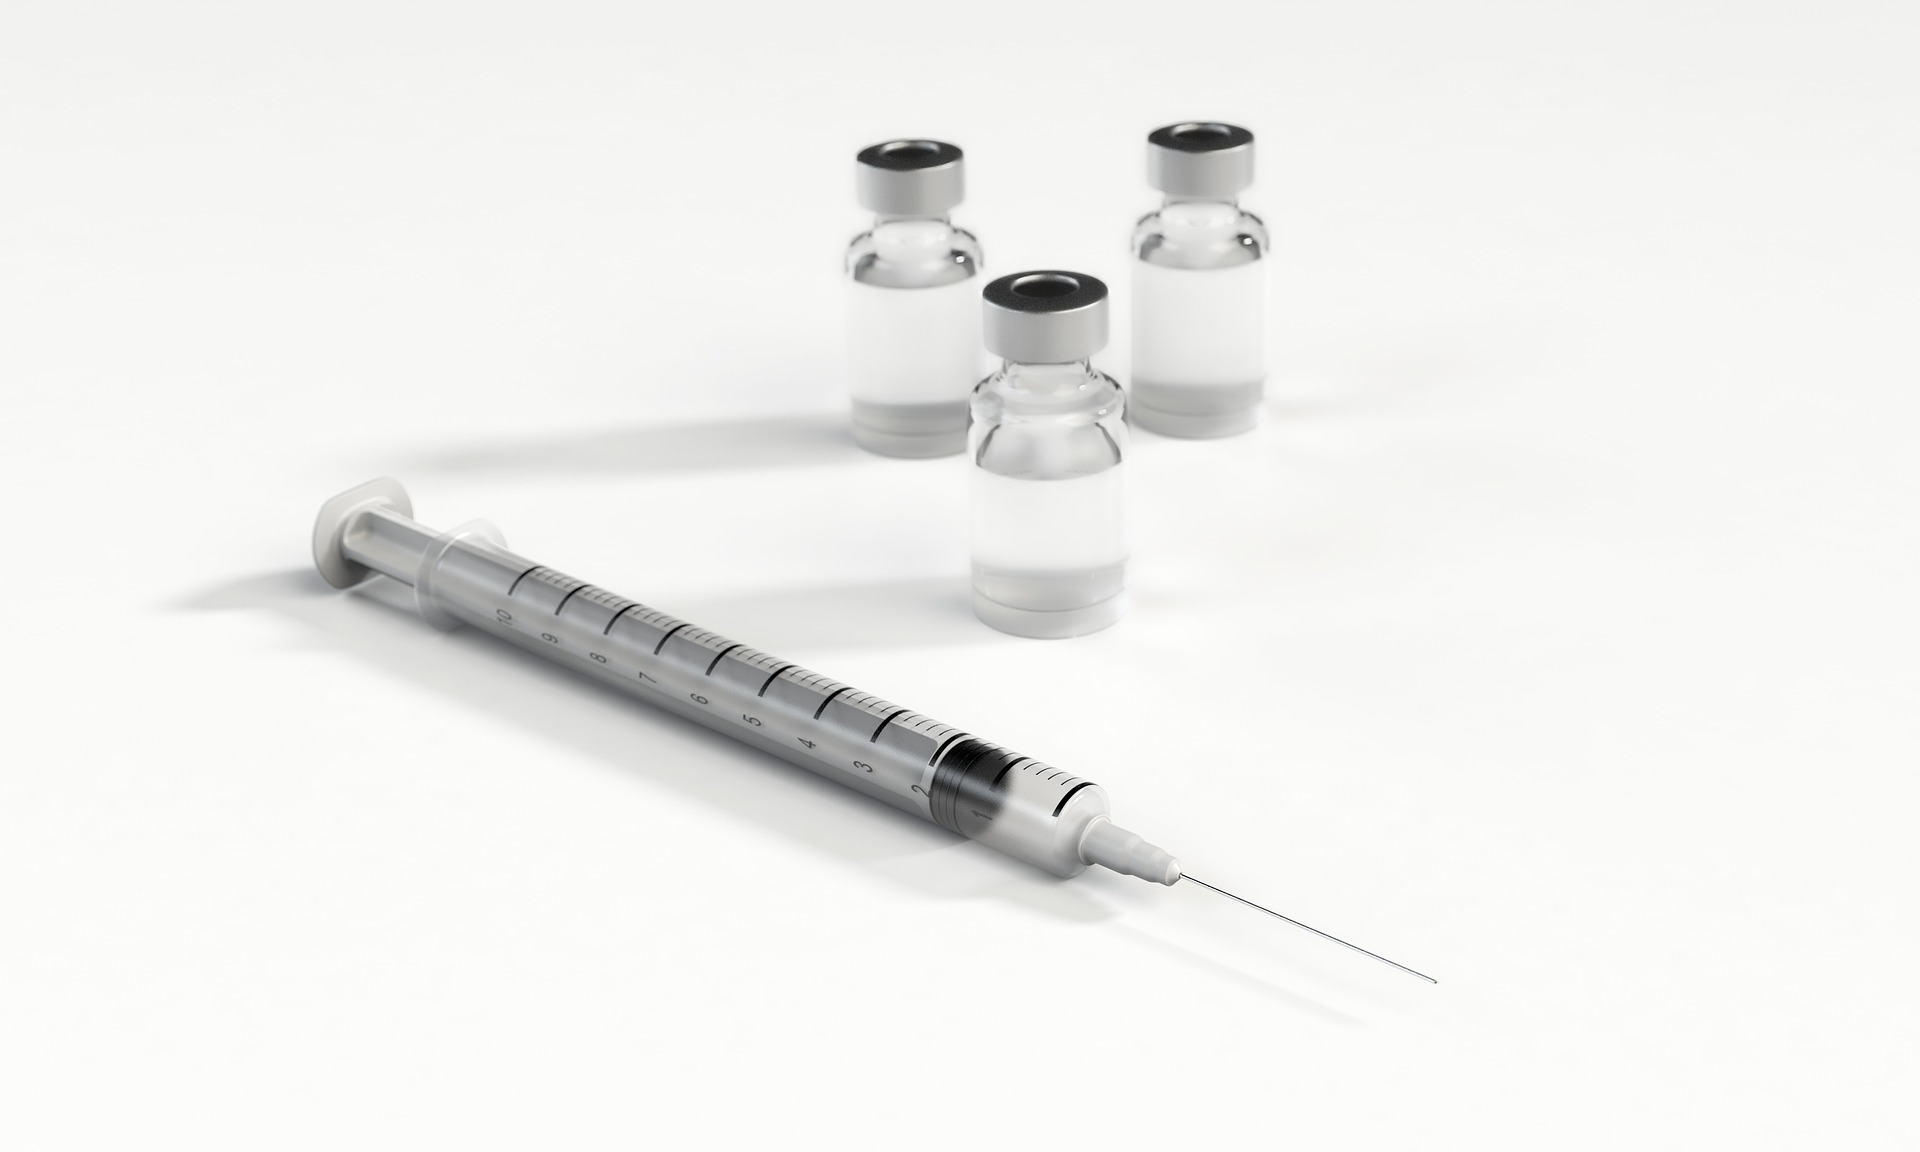
\includegraphics[width = \textwidth]{./images/vaccine}
 \textbf{Estimate:}  The maximum dose of the medication is 26mg.

\end{frame}


\begin{frame}
  \frametitle{Importance of Uncertainty}
       \center 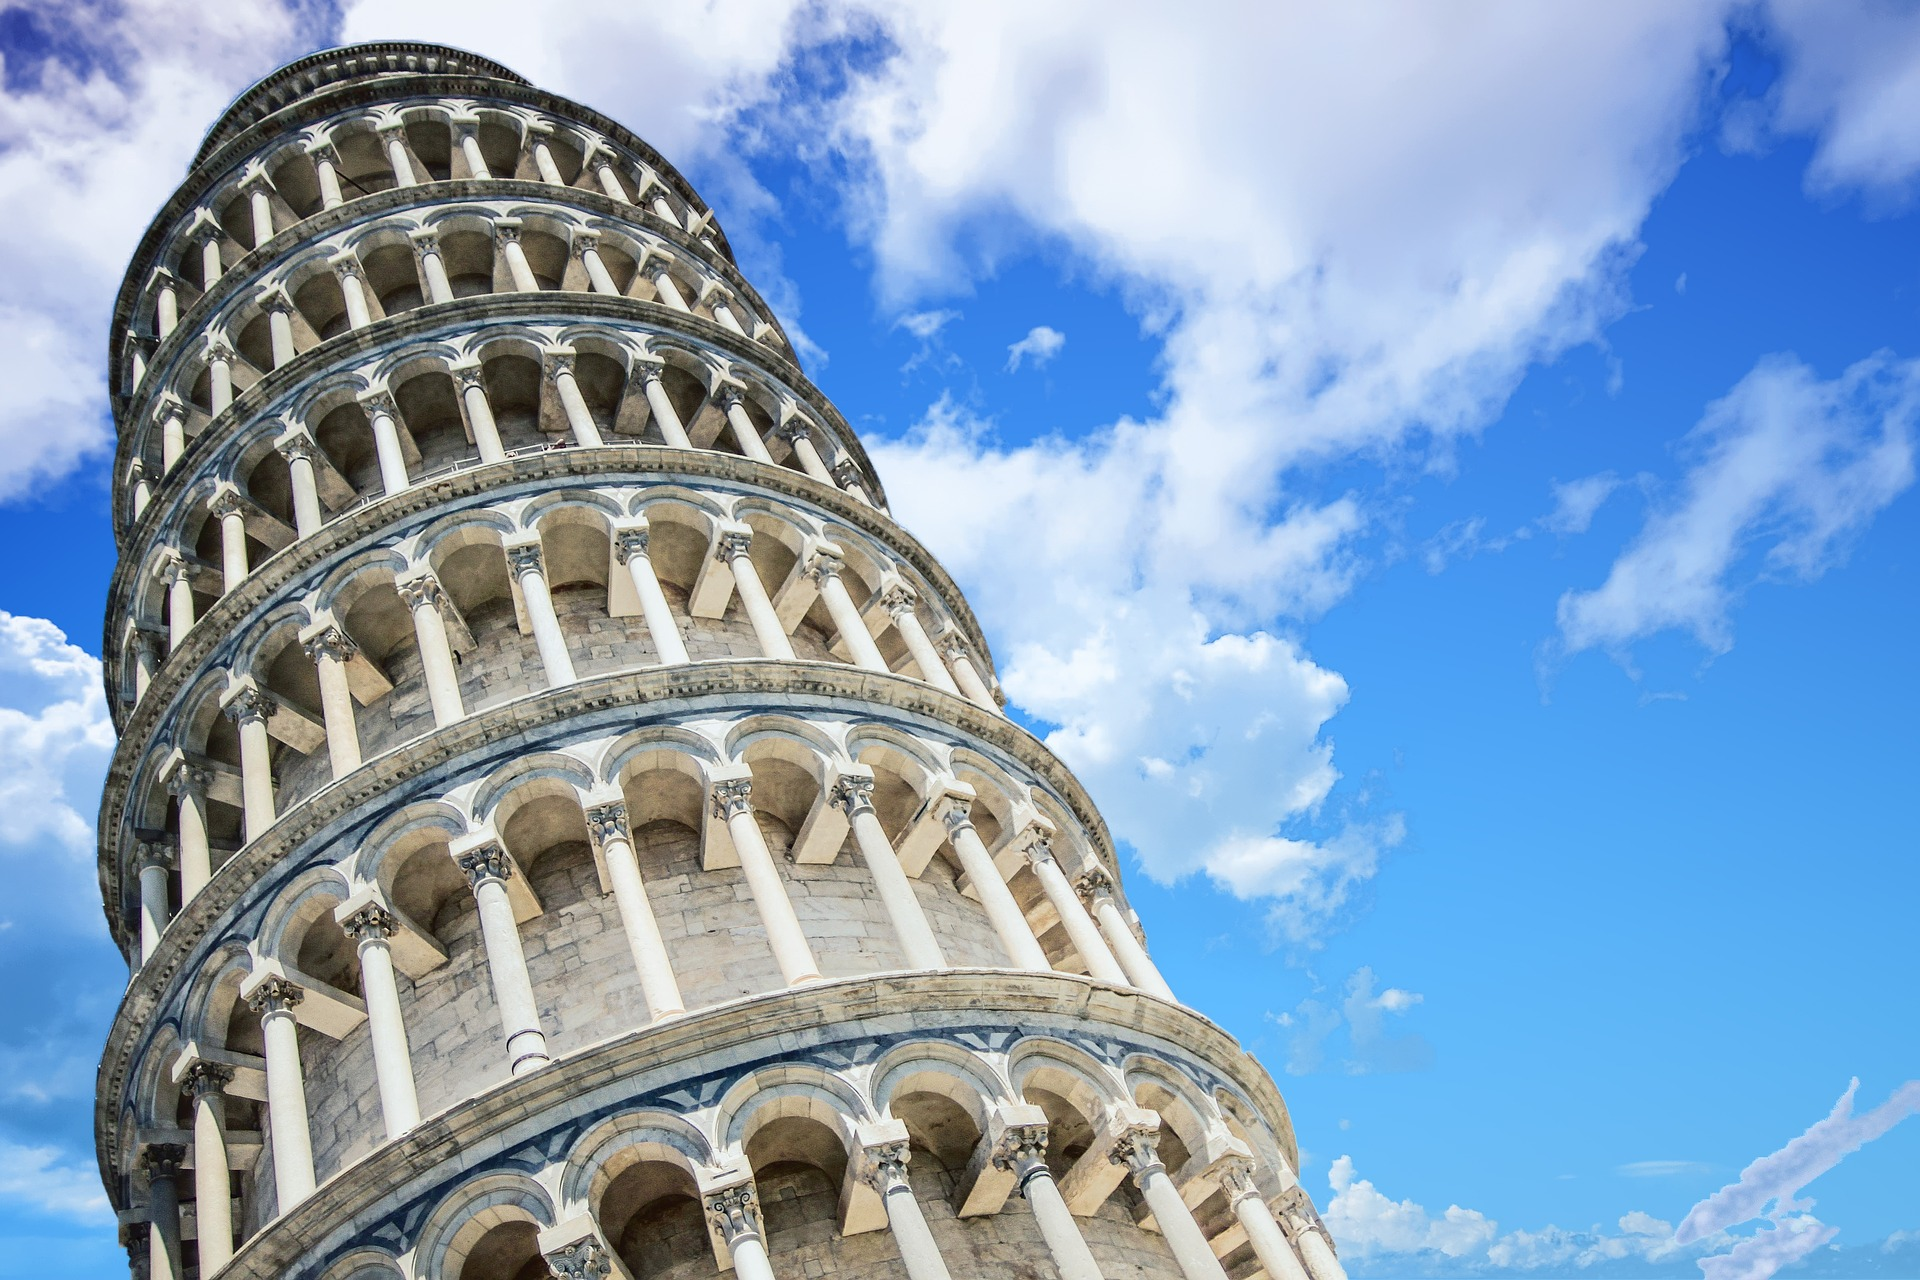
\includegraphics[width = \textwidth]{./images/tower}
 \textbf{Estimate:}  The angle of the tower is 90 degrees.

\end{frame}

\begin{frame}
  \frametitle{The Sampling Distribution of the Statistic}
          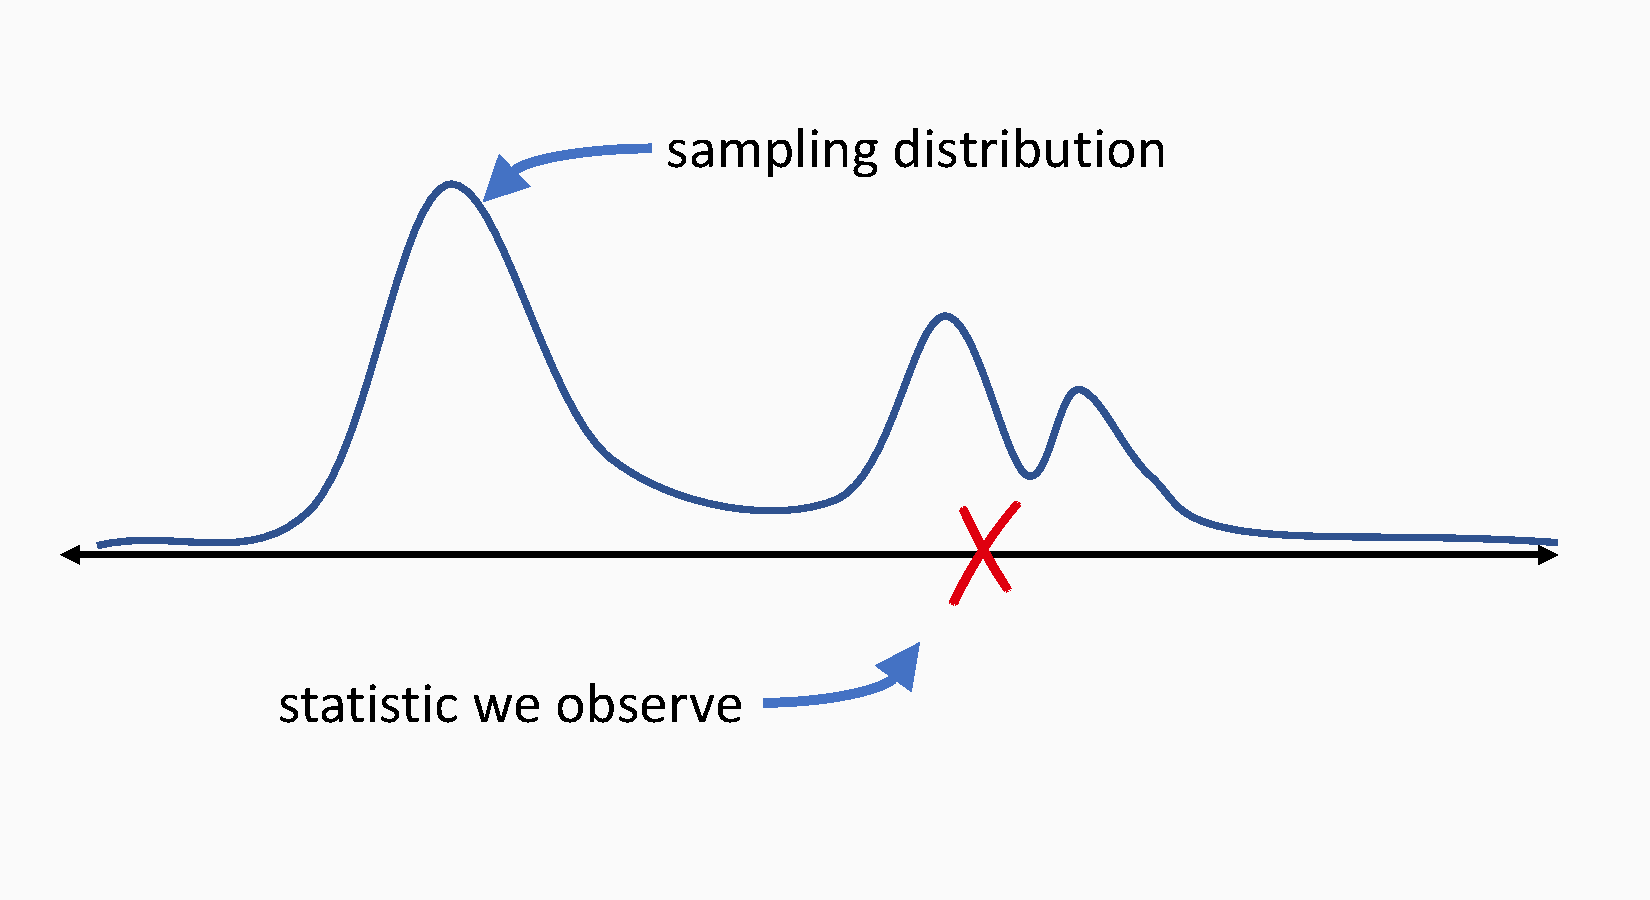
\includegraphics[width = \textwidth]{./images/sampling_distribution}
  \note[item]{Remember that a statistic IS a random variable}
  \note[item]{You get a single number.  But the model says that there are other values that are possible.}
  \note[item]{There is an entire probability distribution over possible values.}
  \note[item]{If we could see this distribution, we could understand how representative our one value is.}
  \note[item]{We could gauge how different it might be from the true parameter.}
  \note[item]{We can't see the sampling distribution, but if i.i.d. holds, we can still learn things about it.}
  \note[item]{A good first question: how spread out is it? standard error = standard deviation of the sampling dist.}
  \note[item]{You can think of the standard error as estimating, if you could run your study over and over, how far apart the values would be on average.  that's an important indicator of uncertainty.}
\pause
  \textbf{Standard Error:} (Estimated) standard deviation of the sampling distribution
\end{frame}


\begin{frame}
  \frametitle{Reporting standard errors}
\note[item]{Really, whenever you report a statistic, you always want to include standard errors.}
\note[item]{unless you have another method of expressing uncertainty.}
\note[item]{There are a couple of ways to include them...}
\begin{enumerate}
\setlength\itemsep{1em}
\item The mean number of mushrooms per pizza was 13.2 (SE  3.6).
\item The time for mice to navigate the maze was 35 $\pm 2$ seconds.
\item \begin{tabular}{c | c}
Vitamin W & Vitamin X \\
\hline
2.3 & 3.4 \\
(0.3) & (0.9)
\end{tabular}
\end{enumerate}

\end{frame}



\section{Standard Errors, The Sample Variance, and Standard
  Deviation}

\begin{frame}
  \frametitle{Many Measures of Dispersion}
  \begin{columns}[t]
    \column{.49 \linewidth}
    \begin{block}{Sample Variance}
      \vspace{4.25em}
    \end{block}

    \begin{block}{Sample Standard Deviation}
      \vspace{4.25em}
    \end{block} 

    \column{.49 \linewidth}
    \begin{block}{Sampling Variance of the Sample Mean} 
      \vspace{3em}
    \end{block} 


    \begin{block}{Standard Error of the Sample Mean}
      \vspace{3em}
    \end{block}
  \end{columns} 
  
  \note[item]{It can seem like we're just making a salad with all
    these concepts!}
  \note[item]{I mean, I am a Berkeley vegetarian, but even I don't like
    variance salads.}
  \note[item]{The \textbf{Sample Variance} is the (de-biased)
    sample-based estimator of the population variance. $V[X] = E[X^2]
    - E[X]^2$ is the
    population, value, and $\hat{V}[X] =
    \frac{n}{n-1}\big(\overline{X^{2}} - \overline{X}^{2}\big)$ is the
    corresponding sample variant.}
  \note[item]{The \textbf{Sample Standard Deviation} is the square
    root of the sample variance.} 
  \note[item]{The \textbf{sampling variance of the sample mean} is a statement
    about how much the same average ``moves'' as a result of
    sampling. This is $V[\overline{X}] = \frac{V[X]}{n}$}
  \note[item]{Finally, the \textbf{standard error} is the square-root
    of the sampling  variance of the sample mean.} 
\end{frame}



\section{Motivating The Central Limit Theorem}

\begin{frame}
\frametitle{Capturing Uncertainty}
Need tools to capture how far off our estimate may be.
\begin{itemize}
\item Standard Error: the (estimated) standard deviation of the sampling distribution of the estimator.
\item But a standard error is just one number...
\end{itemize}

  \note[item]{We've talked about how important uncertainty is.}
  \note[item]{A point estimate by itself isn't all that useful.  we need a way to capture how far off it might be}
  \note[item]{One answer to that is the standard error, which is an estimate for the standard deviation of the sampling distribution of a statistic.}
  \note[item]{But the standard error doesn't capture everything about the sampling distribution.}
  \note[item]{It's just one number.  it can give you a general idea, but can't help you make precise statements about what parameter values are plausible.}
\end{frame}

\begin{frame}
  \frametitle{Uncertainty Example}
    \note[item]{Here's an example.  You want to understand whether vitamin W improves performance on a statistics test.}
  \note[item]{You don't know this, but vitamin W doesn't do anything}
  \note[item]{You estimate the performance, and it's positive, great!}
  \note[item]{But you know that there's uncertainty.  So you're not conviced the effect is really positive}
  \note[item]{You decide on this rule: if the estimate is at least 2 standard errors away from zero, you'll take the vitamin to market.}
  \note[item]{That's actually not a terrible rule of thumb.  This is a very very simplified version of a hypothesis test , but I think there's enough detail to make this point.}
         \center 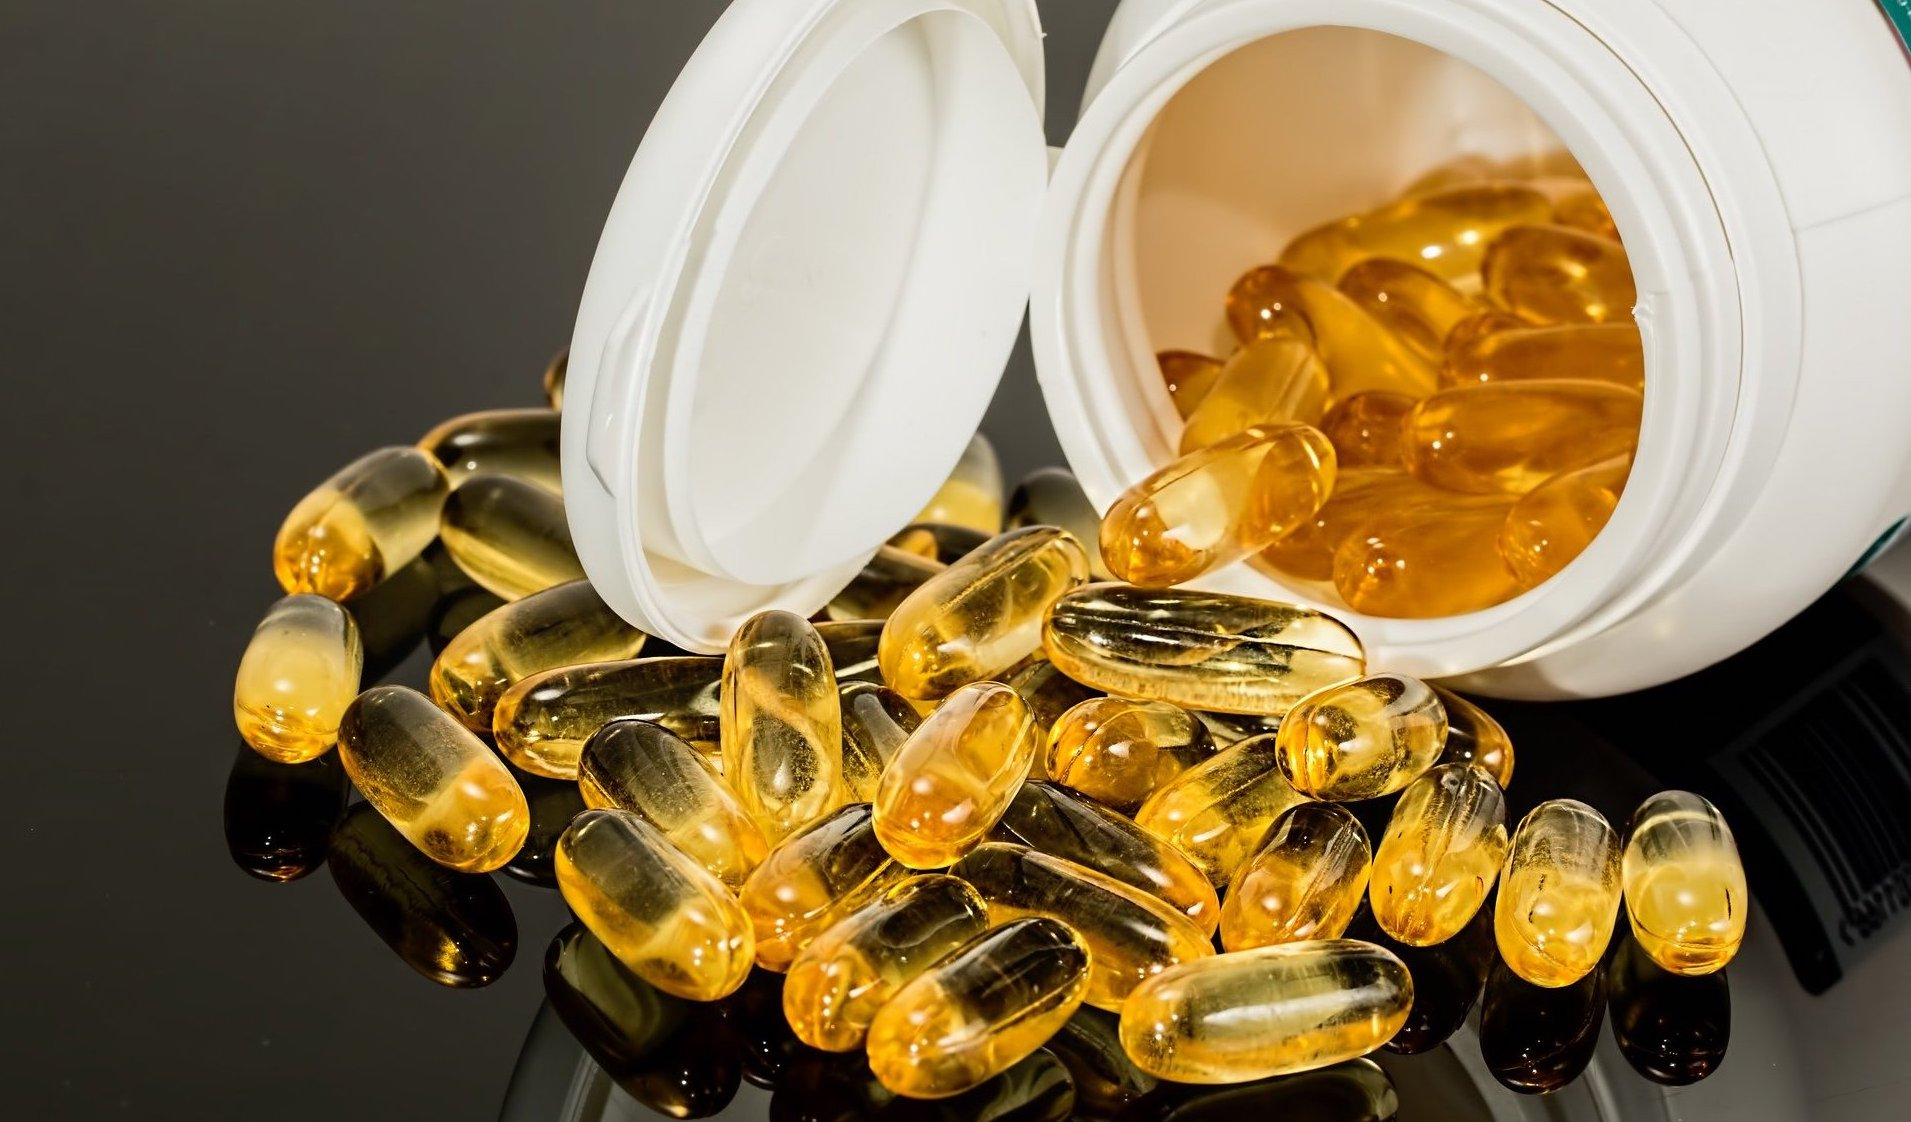
\includegraphics[width = \textwidth]{./images/vitamin}
         \vspace{-.8cm}
\begin{itemize}
\item Hidden fact: Population mean = 0
\item Idea: Market if estimate is 2 standard errors above 0.
\end{itemize}

\end{frame}


\begin{frame}
  \frametitle{The Importance of Shape}
       \center 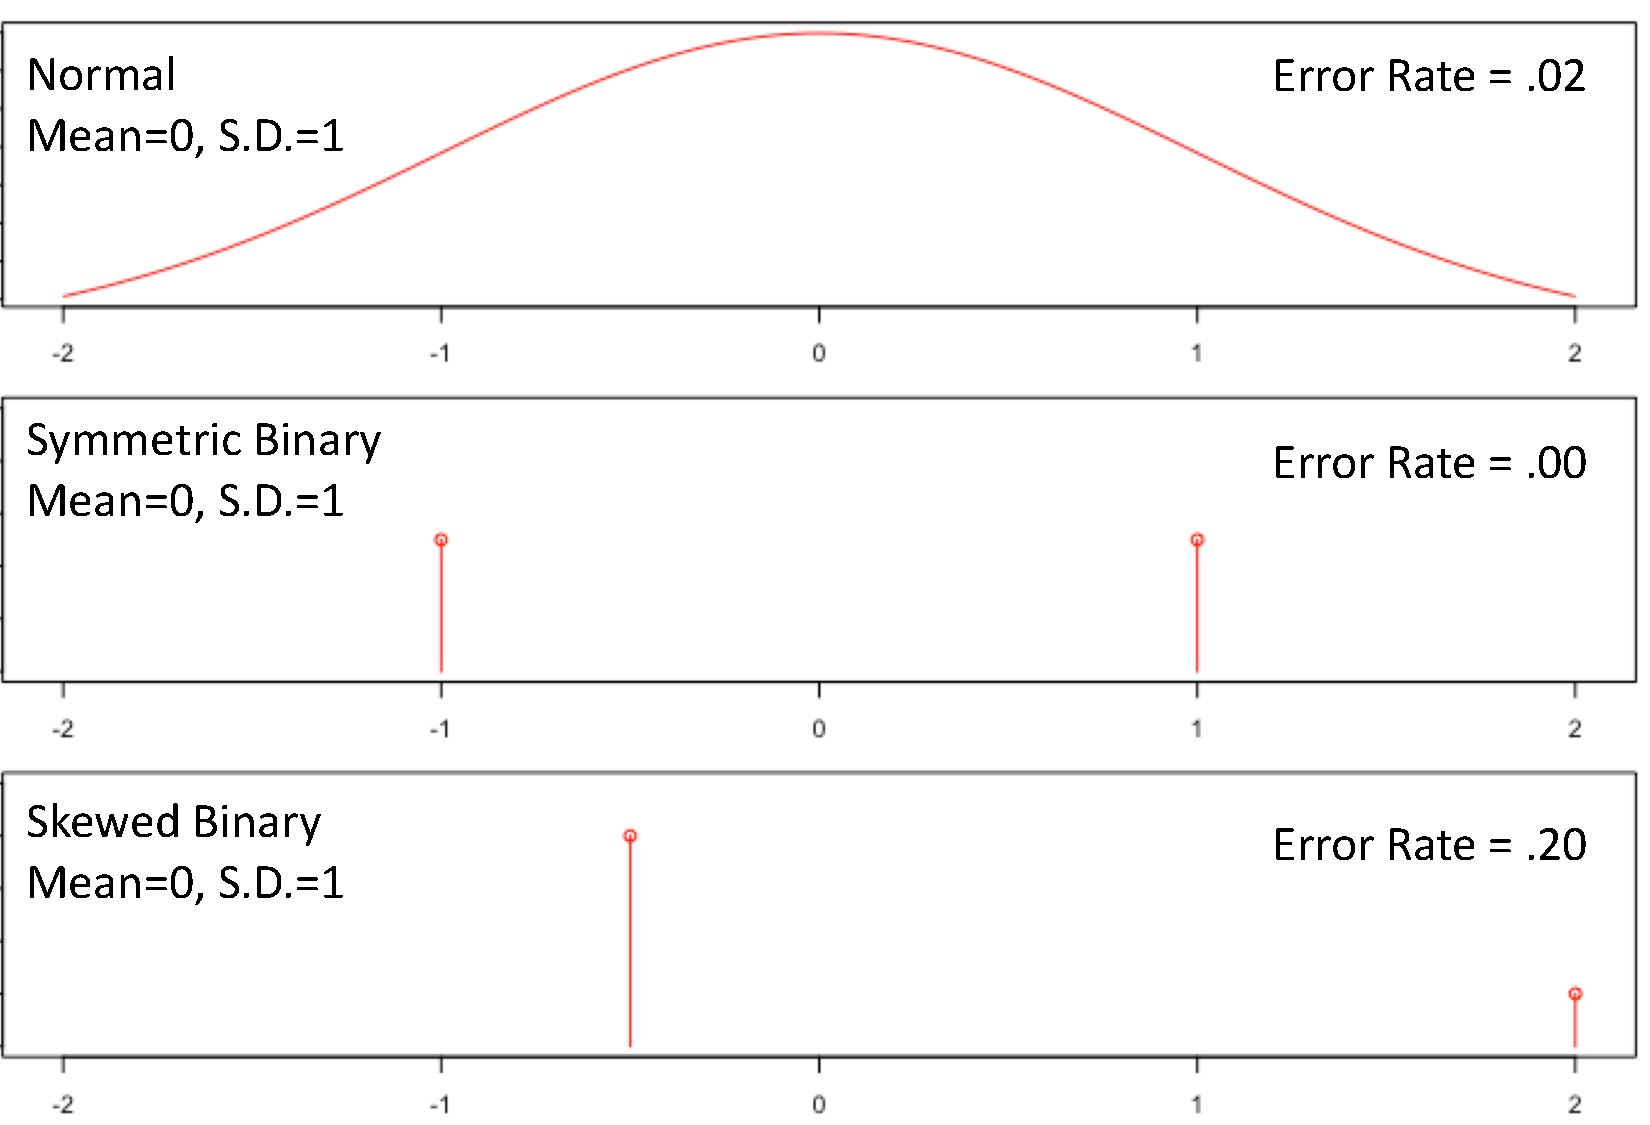
\includegraphics[width = \textwidth]{./images/equal_se}

  \note[item]{Here are three possible sampling distributions for the statistic.  All 3 of them have a mean of 0 and a standard error of 1.}
  \note[item]{So if you get an estimate of 2, you will take vitamin W to market.  and that's a mistake because the true effect is zero.}
  \note[item]{The question is, how likely are you to make a mistake in each case?}
  
  \note[item]{So the shape really matters when we want to express uncertainty more precisely.  That seems like a problem, because there are so many possible shapes out there.}
\end{frame}



\begin{frame}
  \frametitle{The Central Limit Theorem}
  \note[item]{It turns out that a very famous theorem can help us.  It's called the CLT.}
  \note[item]{The CLT says that, yes, there are a lot of possible distributions out there.  If you have a small sample size, the variety is a big problem}
  \note[item]{But as the sample size grows large, the sampling distribution of the sample mean becomes more and more normal.}
  \note[item]{This is great because it's going to unlock a lot of important tools, including confidence interval and hypothesis tests.}
  \note[item]{Because of that, this is often viewed as the most important theorem in all of classical statistics}
  \begin{block}{Central limit theorem (CLT): idea}
    For a \textbf{very broad} class of population distributions, the sampling distribution of the mean becomes approximately normal as the sample size grows large.
  \end{block}
\end{frame}

\section{Reading: The Central Limit Theorem}

\begin{frame}
  \frametitle{Reading: The Central Limit Theorem} 
  \textbf{Note: This is a reading call, we're just placing it here for
    organization.}
  Read pages 108 and 109 of section 3.2.4. There's no \textit{need} to
  read through the demonstration of Slutsky's theorem, but you can if
  you would like.
  \begin{itemize} 
    \item Rather than proving the CLT, we are going to ask you to work
    through a short demonstration against data that we hope will
    convince you of the CLT's effectiveness.
  \item The book is terse in its presentation of when and how the CLT
    applies. We will fill that out when we come back together.
  \end{itemize} 
\end{frame}

 \section{Apply the Central Limit Theorem}

 \begin{frame}
   \frametitle{Apply the Central Limit Theorem}
  \textbf{Note: This is a learnosity activity, just placing it here
    for organization.}
 \end{frame}
 
\section{Central Limit Theorem}

\begin{frame}
  \frametitle{Reminder of Context}
  \begin{itemize} 
  \item The WLLN tells us what happens to the sample mean as $n
    \to \infty$: $$\overline{X} \overset{p}{\to} \E[X]$$
  \item We also know that, as $n \to \infty$, we can generate an
    increasingly good estimate for $\V[X]$ because $$\overline{X^{2}} -
    \overline{X}^{2} \overset{p}{\to} \V[X]$$
    \item For more precise statements about uncertainty, we need the sampling distribution of the statistic.
  \end{itemize} 


  \note[item]{We were really glad when we saw the result of the WLLN.}
  \note[item]{From weak assumptions, we can put together an estimator
    $\hat{\theta}$ that converges in probability to the expected
    value. But this is only for a single point on the distribution.}
  \note[item]{What if we want to know more information about this
    estimator?} 
\end{frame}

\begin{frame}
  \frametitle{Convergence in Distribution}
    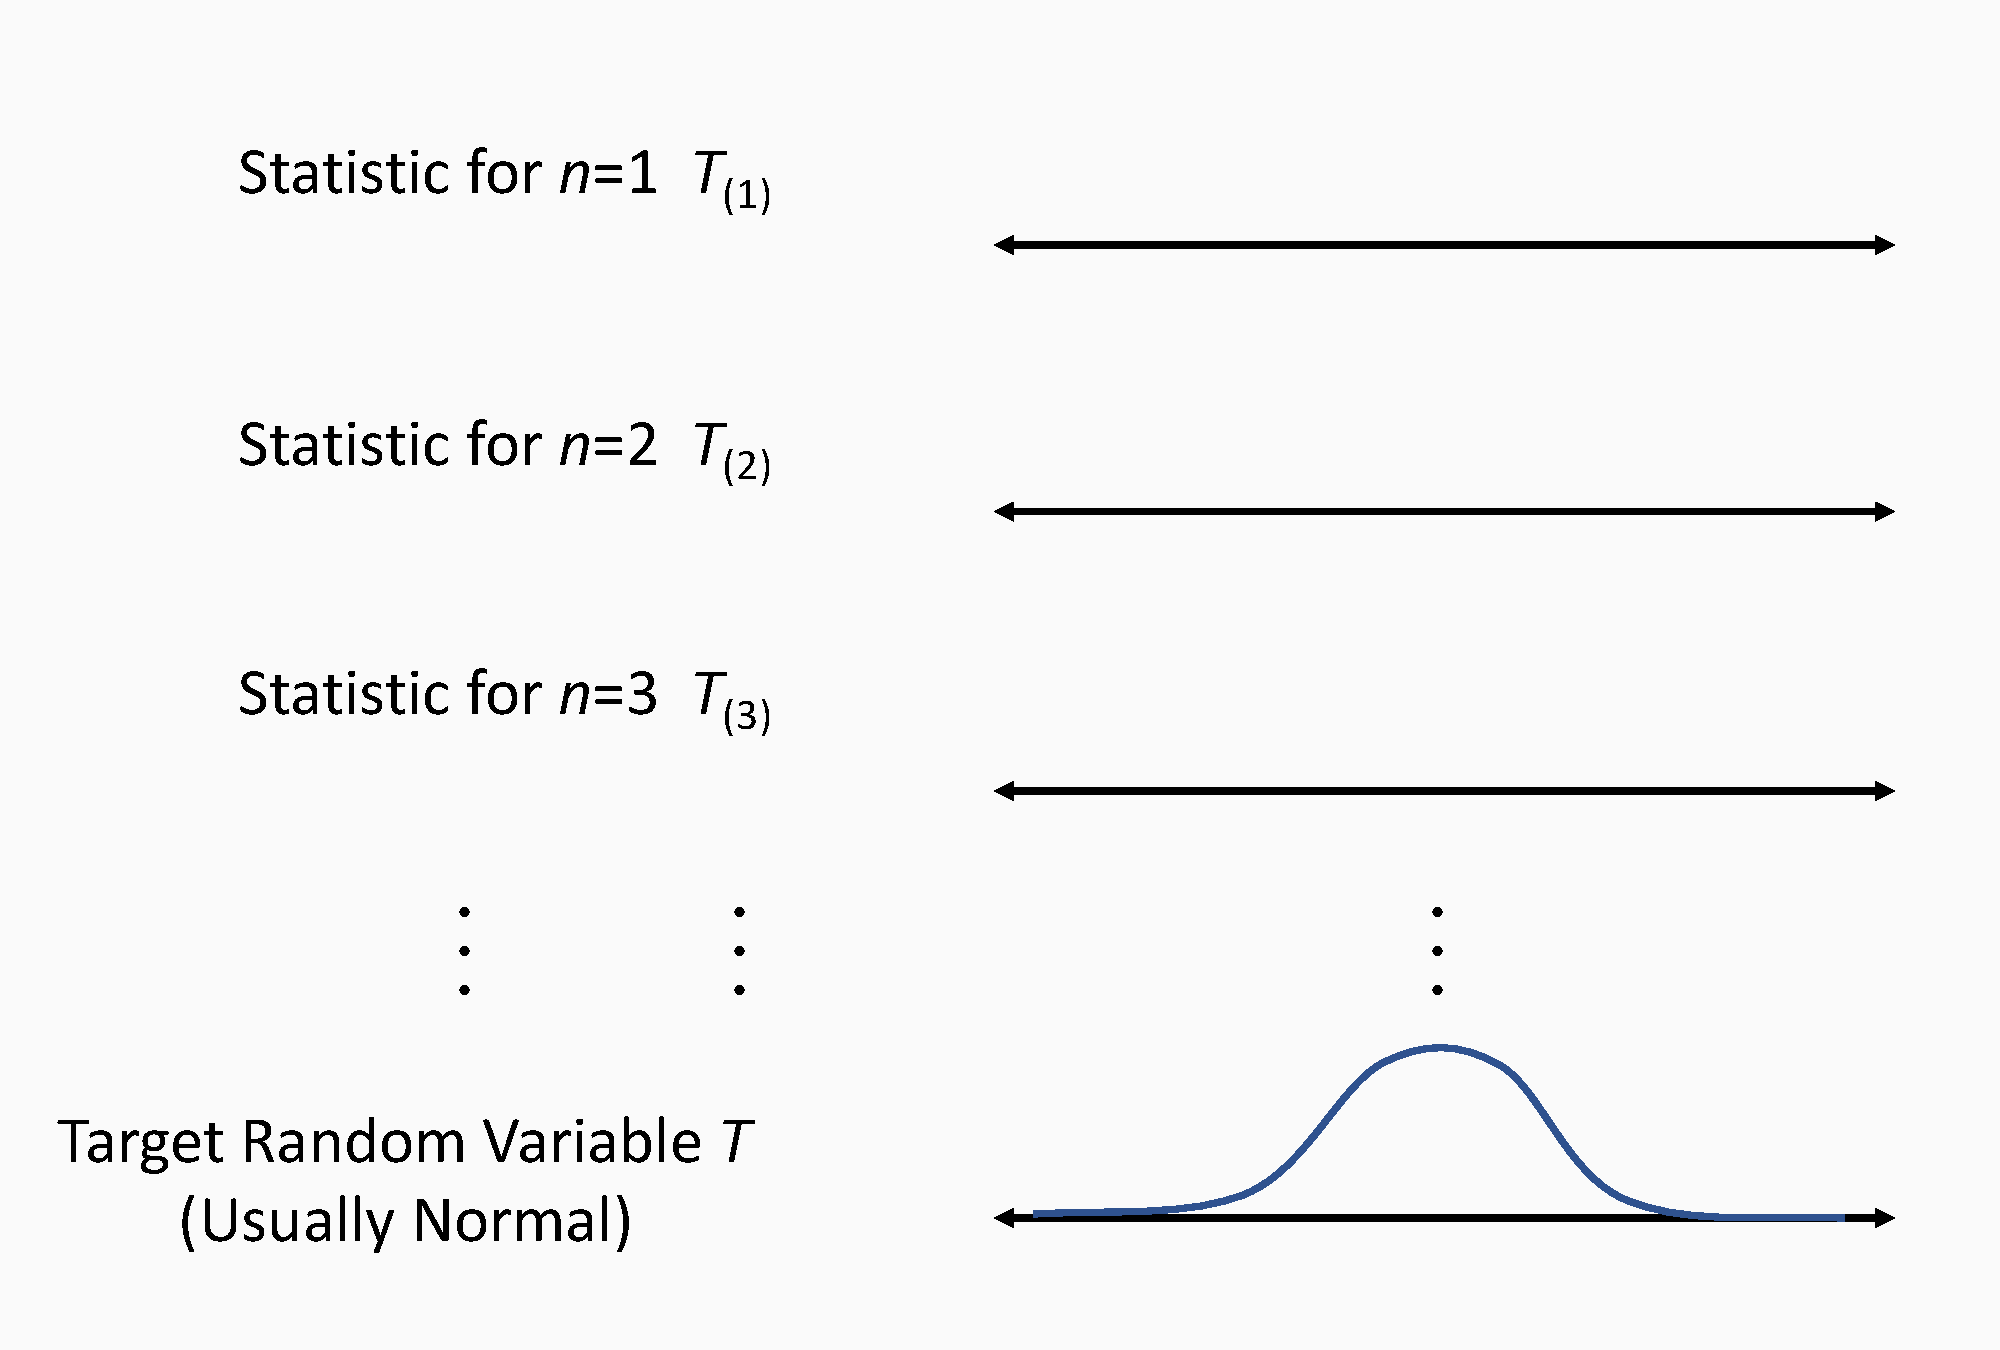
\includegraphics[width=\linewidth]{images/convergence_in_d}
  \note[item]{Let's build out the idea of \textit{convergence in
      distribution} (image on next slide)}
  \note[item]{Suppse you have a sequence of random variables, for now,
    it will be a set of sample means.}
  \note[item]{First, suppose that you take a sample of size 1, and
    return the average. What will you see?}
  \note[item]{Then, suppose that you take a sample of size 2, and
    return the average. What will you see?  Will this larger sample
    have a larger or a smaller sampling variance of the mean? (This
    is the WLLN claim).}
  \note[item]{The idea of convergence in distribution, is
    that as you go along the sequence of distributions, the shape
    \textit{at every point} becomes more and more like the
    target; this is why it is defined in terms of CDF.}
  \note[item]{Convergence in distribution is much stronger than just a
    single point converging like we had for the
    WLLN. $\overset{p}{\to}$ covers a  single point or  
    moment. $overset{d}{\to}$ is much much stronger.} 
  \note[item]{The whole distribution not just a central tendency for
    example, converges to 
    the mean.}   
\end{frame}

\begin{frame}
  \frametitle{Convergence in Distribution}
  \note[item]{Here's the statement, and the thing to notice is that the actual statement of convergence is in terms of the CDFs}
  \note[item]{You might hope it was about pdfs, but that's not possible.  for example, if you have a discrete population, you can never have a continuous statistics}
  \note[item]{Also, every random variable in the world has a cdf, so that makes this more universal.}
  
  \begin{block}{Definition: Convergence in distribution}
  Let $(T_{(1)}, T_{(2)}, T_{(3)}, ...)$ be a sequence of random variables, with cdfs  $(F_{(1)}, F_{(2)}, F_{(3)}, ...)$, and let $T$ be a random variable with cdf $F$.  Then $T_{(n)}$ \textit{converges in distribution} to $T$ if, for all $t\in \R$ at which $F$ is continuous,
  $$\lim_{n \rightarrow \infty} F_{(n)} (t) = F(t).$$
  We denote this as $T_{(n)} \overset{d}{\rightarrow} T.$ 
  \end{block}
\end{frame} 

% \begin{frame}
%   \frametitle{Convergence in Distribution}
%   \begin{block}{Convergence in Distribution}
%     Let $(T_{(1)}, T_{(2)},T_{(3)},...)$ is a sequence of random variables with CDFs $(F_{(1)}, F_{(2)},F_{(3)},...)$.
%     Let $T$ be a random variable with CDF $F$.
%     Then $T_{(n)}$ converges in distribution to $T$ if ($\forall t \in \R$ at which $F$ is continuous),
%     We write this as $T_{(n)} \overset{d}{\to} T$
% %    If, as $n\to\infty$ the CDF, $F_{n}(t)$ of a sample of the random variable, $T$
% %    tends to the CDF of the population, $F(t)$, then we say that the sequence
% %    \textit{converges in distribution}, or has an \textit{asymptotic
% %      distribution} that is just $T$. 
%   \end{block}
%   \note[item]{\paul{Here's the actual statement of convergence in distribution.  You can
%       see that the convergence is in terms of the cumulative
%       distributions.  The cumulative distributions converge on the
%       target, for every single point.}} 
% \end{frame}

\begin{frame}
  \frametitle{The need to Standardize}
  \centering
  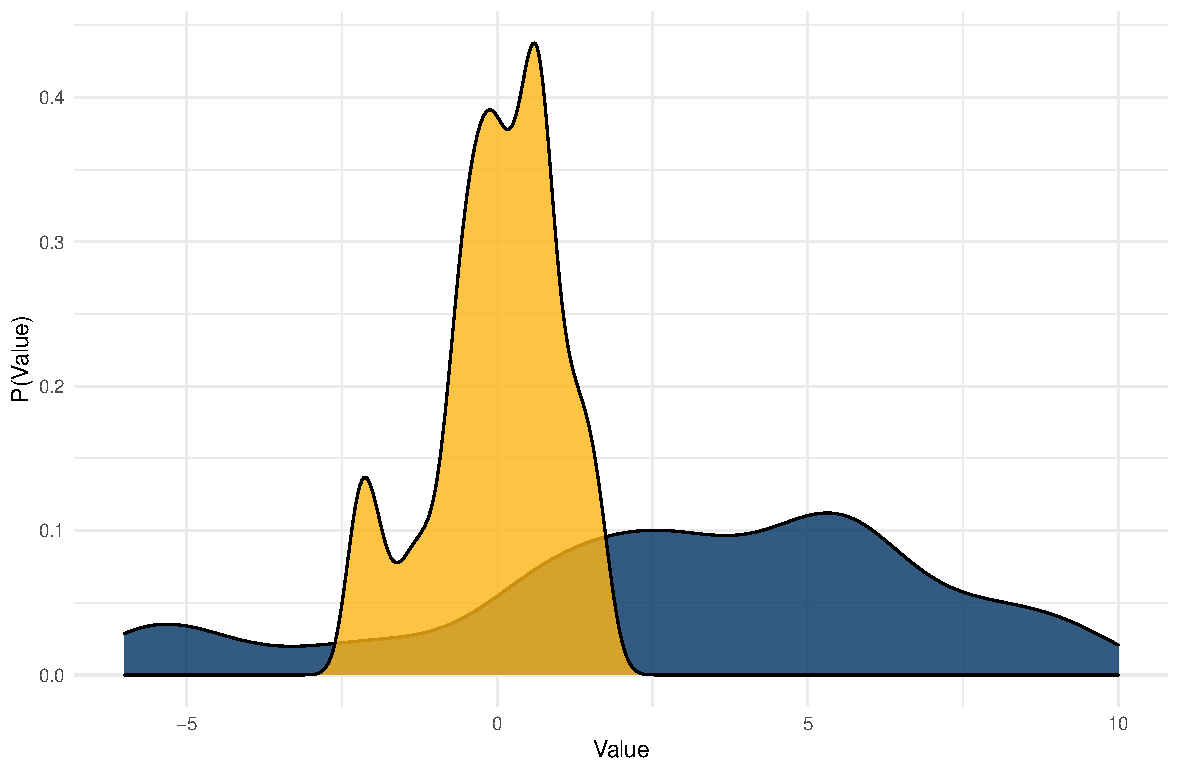
\includegraphics[width=\linewidth]{./images/standardizing_values}
  \note[item]{We want to say that the distribution of the sample mean converges in distribution to the normal, but there's one more wrinkle.}
  \note[item]{Remember that as n increases, the distribution gets thinner and thinner.}
  \note[item]{The variance decreases as 1/n}
  \note[item]{So we can't just look at the raw distribution, which approaches a spike.  We have to stretch it back out so that the width is a constant.}
\end{frame}

\begin{frame}
  \frametitle{Standardizing the Sample Mean}
  \note{Recall, $$\V\big[\overline{X}\big] = \frac{\V[X]}{n}$$ and
    so
    $$\sigma\big[\overline{X}\big] = \sqrt{\frac{\V[X]}{n}} =
    \frac{\sigma}{\sqrt{n}}.$$}
  \begin{block}{Definition: Standardized sample mean} 
    For IID random variables $(X_1,X_2,...,X_n)$ 
    with finite $\E[x] = \mu$ and finite $\V[X] = \sigma^2$,
    then \textbf{the standardized sample mean} is:
    $$
    Z = \frac{\left(\overline{X} - \E\big[\overline{X}\big]
      \right)}{\sigma\big[\overline{X}\big]} =
    \frac{\sqrt{n}\big(\overline{X} - \mu\big)}{\sigma}.
    $$
  \end{block}
  \begin{itemize}
\item The standardized sample mean always has mean 0 and standard deviation 1.
\end{itemize}

\end{frame}

\begin{frame}
  \frametitle{The Central Limit Theorem}
  \note[item]{With all that out of the way, we can finally state the CLT}
  \begin{block}{The Central Limit Theorem}
    Let $(X_1,X_2,X_3,...)$ be a sequence of i.i.d. random variables with finite mean $\E[X] = \mu$ and finite variance $\V[X] = \sigma^2$,
    $$
    Z =    \frac{\sqrt{n}\big(\overline{X} - \mu\big)}{\sigma}  \overset{d}{\to} N(0,1)
    $$
    % $$
    % which is the equivalent to
    % $$
    % \sqrt{n}(\overline{X} - \mu) \overset{d}{\to} N(0, \sigma^{2})
    % $$
  \end{block}
  \note[item]{To summarize: As long as n is large enough,
    then the mean, $\overline{X}$, has an approximately normal
    distribution.}
    \note[item]{It doesn't matter what the population distribution looks like.}
    \note[item]{This means that we can run hypothesis tests and make precise statements about uncertainty.}
\end{frame}

\begin{frame}
  \frametitle{Generality of the CLT}
The CLT applies to:
    \begin{itemize}
    \item Continuous Random Variables
    \item Discrete Random Variables
    \item Symmetric Random Variables
    \item Asymmetric Random Variables
  \end{itemize}
 Only Requirements:
 \begin{itemize}
\item Data points are IID.
\item Population has finite variance.
\end{itemize}
Versions of the CLT exist for many other statistics.

\end{frame}


\begin{frame}
  \frametitle{What Sample Size is Enough?}
  The CLT works in the limit as
    $n\to\infty$.  What can we say for a finite $n < \infty$?
    \note[item]{When you were working with a normal underlying
      distribution, how quickly with a sample average move
      $\overset{d}{\to} N$? $n = 1$ will work!}
    \note[item]{If two distributions have the same $V[X]$ will they
      $\overset{d}{\to}N$ at the same rate?}
    \note[item]{There's a general rule of thumb that for $n > 30$,
      the CLT will work.}
      
      \begin{itemize}
\item Rule of Thumb: $n=30$ for CLT to "kick in."
\item Reality: Convergence depends on how non-normal population is.
\begin{itemize}
\item A normal population requires $n=1$.
\item Highly skewed distributions may require $n=100$, $n=1000$, or more.
\end{itemize}

\end{itemize}

\end{frame}



\section{Learnosity: When Does the CLT Apply?}

\begin{frame}[t]
  \frametitle{Where and When Does the CLT Apply? Part III} 
  
  \textbf{Which of these random variables has an approximately normal distribution because of the CLT?}
  \begin{itemize}
  \item $X=$ hours spent by one individual on a 203 homework
    assignment
  \item $X=$ average hours spent by randomly assigned study groups of
    size 4 on the same 203 homework
  \item $X=$ number of barks by a dog named Rex for a one-hour
    period at night
  \end{itemize}
\end{frame}

\begin{frame}[t]
  \frametitle{Where and When Does the CLT Apply? Part III} 
  
  \textbf{Which of these random variables has an approximately normal distribution because of the CLT?}
  \begin{itemize}
  \item $X=$ total number of barks by a neighborhood of dogs
    for a one-hour period at night
  \item $X=$ age of a randomly selected MIDS student
  \item $X=$ average of sample of 10 randomly selected
    MIDS students
  \item$X=$ VADER sentiment of a sample of 100 SMS
    messages
  \end{itemize}
\end{frame}

\section{The Plug-In Principle}

\begin{frame}
  \frametitle{The Plug-In Principle}
  
  \note[item]{I want to discuss this idea of the Plug-In principle}
  \note[item]{The book uses it a lot, but it also glosses over the details}
  \note[item]{Now you've seen a few estimators, and you may start to notice a pattern...}
  
  \note[item]{If you want a function of the population variance, you can plug the sample variance into the function}
  \note[item]{So statisticians started to notice, hey, if we just plug in these sample analogues, we seem to get good estimators.}
  \note[item]{Is this just an accident?  Or is there something deeper going on?  Can we use this to find estimators for more parameters?}


  \begin{itemize}
  
  \item Want mean of population $\rightarrow$ Mean of sample.
  \item Want variance of population $\rightarrow$ Variance of sample.
  \item Want $f(E[X], V[X])$? $\rightarrow$ $f(\bar X, \hat V(X))$
  \end{itemize}
  \center   See the Pattern?
\end{frame}


\begin{frame}
  \frametitle{The Plug-In Principle}
    \begin{columns}
    \column{\dimexpr\paperwidth}
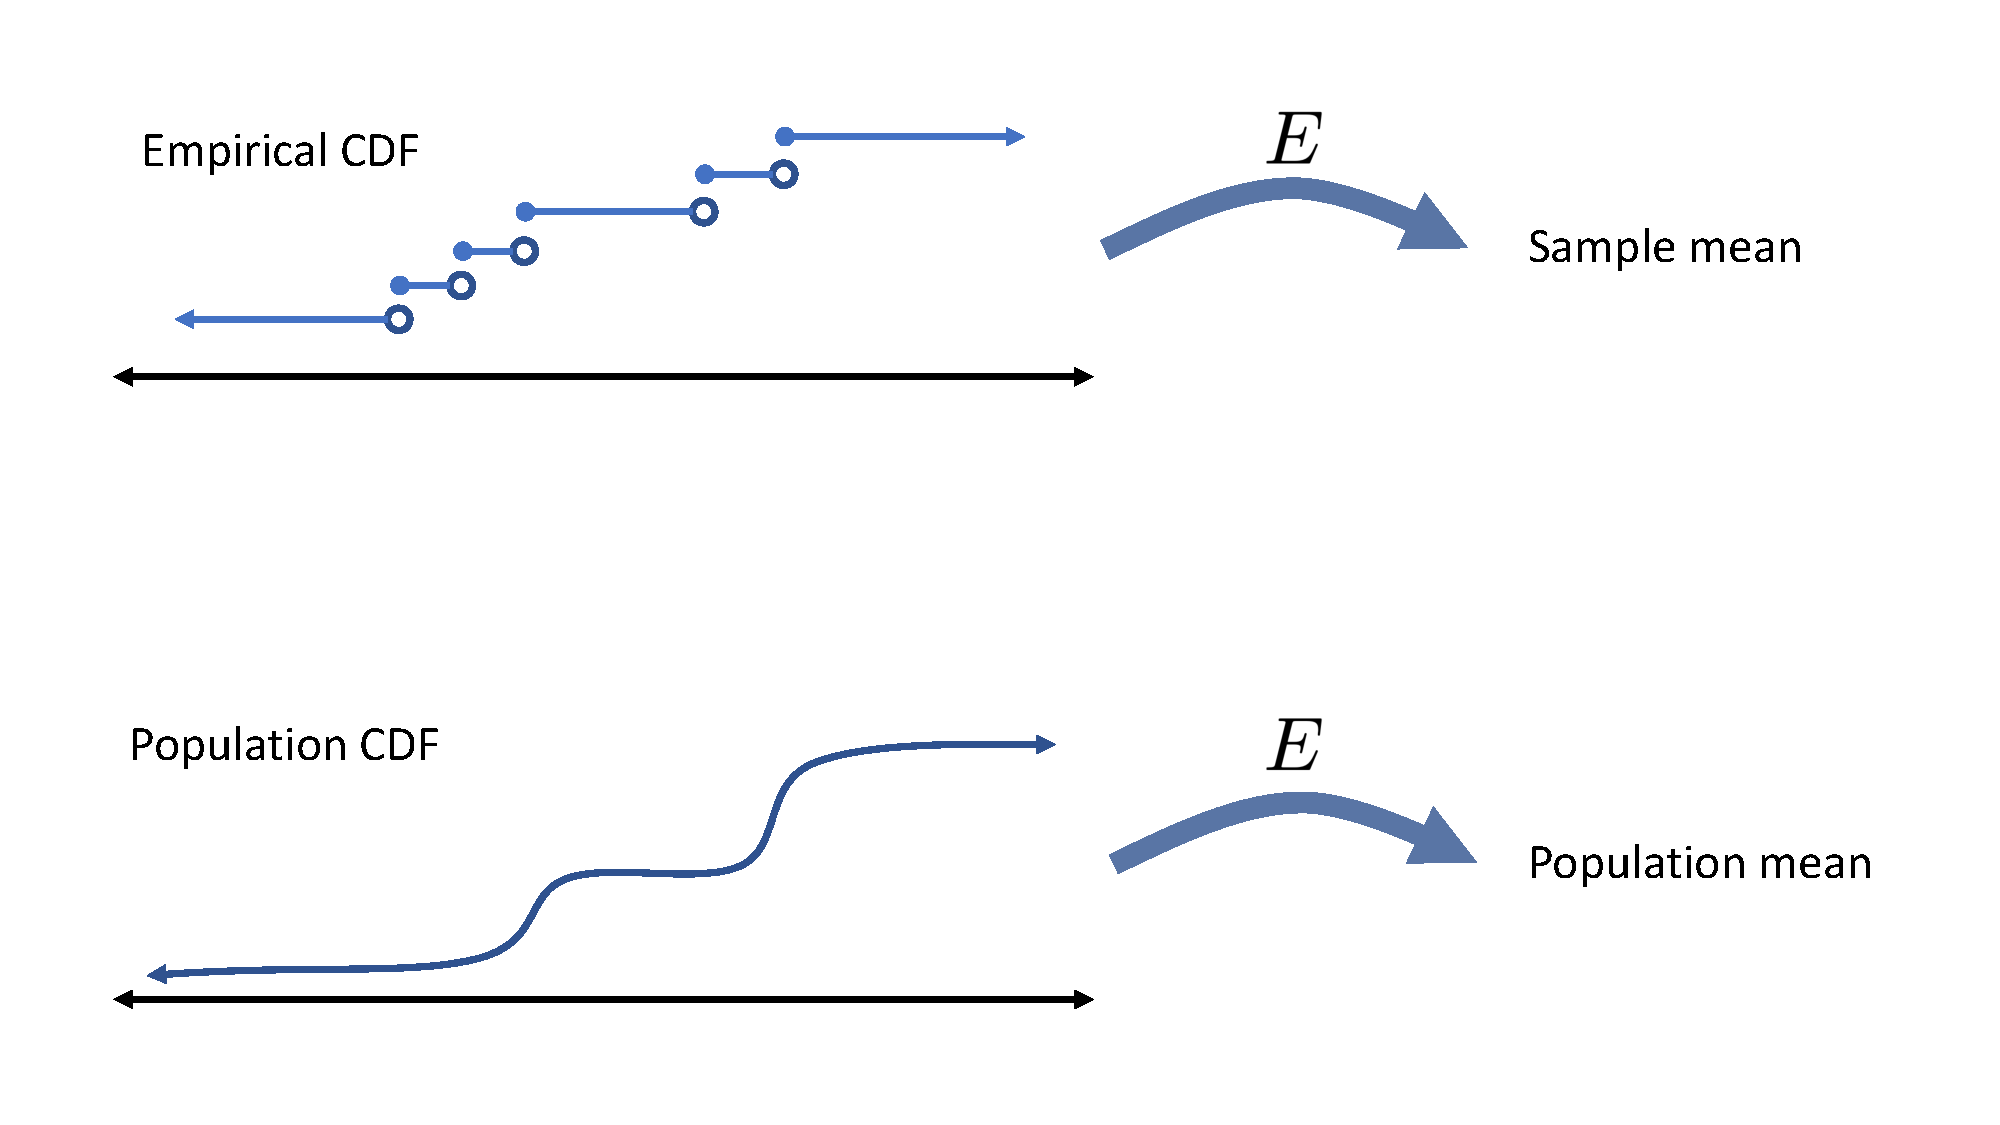
\includegraphics[width=\textwidth]{./images/plug-in}
  \end{columns}
\note[item]{It turns out, yes, there is something going on}
\note[item]{At the bottom, we have a population, represented as a CDF.  We apply expectation to it, to get the population mean}
\note[item]{Now at the top, we have our sample of data, represented by the empirical CDF.  Well, if you take the empirical distribution and apply expectation to it, you get the sample mean.}
\note[item]{What's key here, is that these expectations are exactly the same operator!  You really need to take measure theory to prove this, but hopefully that seems believable}
\note[item]{Now, what happens when $n \rightarrow \infty$?}
\note[item]{We know the empirical CDF converges in distribution on the population CDF.}
\note[item]{We need the expectation operator to be continuous, and that's not easy to define here.  but if it's smooth enough, as the empirical cdf approaches the true cdf, it makes sense that the sample mean approaches the population mean in probability. }
\note[item]{This works a lot of the time.  For a really large class of operators, if you plug in the empirical cdf for the true one, you get a consistent estimator.}
\note[item]{But that's not all.  these estimators are consistent, and they are also asymptotically normal}
\note[item]{That's harder to demonstrate, but here's a hint.  if you look at a point on the CDF function, you can write it as a sample mean - you add a 1 for every point to the left, an 0 for every point to the right.  So the distribution of this point approaches the normal.  So you can maybe believe that if the deviations are small enough, when you pass them through the expectation, you get another normal sampling distribution.}
\note[item]{So that's the plug-in principle.  It's pretty important, because it's also the basis for bootstrap theory.  It does take some advanced math to check that it actually applies to your estimator.  So we won't prove things with it in this class, but it's good to know that it exists, and we will use it to come up with ideas for estimators.}


\end{frame}

\section{Reading Assignment}

\begin{frame}
  \frametitle{Reading Assignment}
  \textbf{Only if you're interested,} read section 3.3 - 3.3.1 to learn more about the Plug-In Principle. 
\end{frame}


\section{Asymptotic Theory}

\subsection{Asymptotics Rescue Data Science}

\begin{frame}
  \textbf{Across a range of applications, small samples are problems.}
  \note[item]{Tie the problems back to the small-sample bias of the
    Plug-In Sampling Variance}
  \begin{itemize}
  \item If we've got a \textit{lot} of data, though, we can rely on
    weaker requirements
  \item Asymptotic properties of estimators ask the question,
    \textbf{What happens when we have a lot of data?} 
  \item In general, as $n\to\infty$, does $\hat{\theta}$ converge in distribution or
  probability to something that is useful or desirable? 
  \note[item]{\paul{Love the intro!}}
  \note[item]{\paul{Is it possible to give some taste of what useful or desirable means, or does that take too long?  I know it would have to be vague.   We don't really expect to find perfectly normal distributions in the real world.  We can't just assume that hair length or income is normal and fit a normal curve to data, nobody would believe our models.  With asymptotics, we know that our statistics follow simple distributions we know how to analyze.  }}
  \end{itemize} 
\end{frame}
 
\subsection{Reading: Asymptotics}

\begin{frame}
  \frametitle{Reading: Asymptotics}
  \textbf{Note: This is a READING CALL. We're placing it here for
    organization.} 
  \begin{itemize}
  \item The interested student can read pages 111-114.
  \item But, we might recommend skipping it if you're constrained. 
  \item The take home is that there is an asymptotic statement of:
    \begin{itemize}
      \item Being Normally Distributed 
      \item SE, MSE and Efficiency 
      \item Sampling Variance and Sampling Standard Error
      \end{itemize}
    \end{itemize} 
\end{frame}
 
% \subsection{Reading: Asymptotic Variance and Standard Error of the Sample Mean} 

% \subsection{Asymptotic Variance and Standard Error of the Sample Mean} 
 
\subsection{Reading: The Plug-In Principle}

\begin{frame}
  \frametitle{Reading: The Plug-In Principle}
  \note[item]{We're not going to lie to you... this is a challenging
    section to read.}
  \note[item]{A couple of notes are in order.}
  \begin{itemize}
    \item $F(x)$ is the cumulative distribution function, the \textit{CDF}
    \item $f(x)$ is the probability distribution function, the \textit{PDF}
    \item $\hat{F}(x) \not= F(x)$ and $\hat{f}(x) \not= F(x)$
     \note[item]{When showing the estimated distributions, note that
       they're not the same as the true distributions.} 
     \item As $n\to\infty$ we hope that $\hat{F}(x)
       \overset{d}{\to}F(x)$ and $\hat{f}(x)\overset{d}{\to}f(x)$.
       \note[item]{This is an important reminder to read the math
         aloud, converting the notation to its language equivalent.} 
      \note[item]{When you asked earlier, ``But where do these
        functions come from?'' the answer is, we estimate them! Here!
        They come from here!} 
  \end{itemize} 
\end{frame}

\subsection{The Plug-In Principle} 

\begin{frame}[t]
  \frametitle{The Plug-In Principle}
  \begin{block}{Expectation and Variance Functionals}
    You \textit{know} what the processes for calculating an expectation
    and variance are.
    \begin{align*}
      E[X] &= T_{E}(F) = \int x \cdot dF(x) \\
      V[E] &= T_{V}(F) = \int (x - E[X])^{2} \cdot dF(x)
    \end{align*}
  \end{block}
  These are the \textit{statistical functionals} for expectation and
  variance.
  \note[item]{You might be annoyed that we're dealing with $dF(x)$ --
    \textit{the derivative of the cumulative distribution function} --
    I was! But this is the only thing that we've got the ability to
    estimate empirically.}
  \note[item]{\paul{This is a Lebesgue integral, and I think the dF
      is fair to replace with f(x) dx if X is continuous, but the
      integral is defined for any measure on R.  I honestly don't
      think the notation is helpful to our students.  You don't
      really need the notation, all that's really needed is to point
      out that expectation and variance are functions of F, which
      should be clear because you can't have one value of F and two
      values for expectation.  }} 
\end{frame}

\begin{frame}
  \frametitle{The Plug-In Principle (cont.)}
  
  \begin{block}{Plug-In Estimators} 
    For i.i.d. random variables $X_{1}, X_{2}, \dots, X_{n}$, with a
    common CDF $F$, the plug in estimator for $\theta = T(F)$ is just
    $\hat{\theta} = T(\hat{F})$.
    \begin{align*}
      \hat{E}(X) &= T_{E}(\hat{F}) \\
                 & = \sum x \cdot \hat{f}(x) \\
                 & = \sum x \cdot \frac{I(X_{i} = x)}{n} \\
                 &= \frac{1}{n} \sum x \\ 
                 &= \overline{X} \\ 
    \end{align*} 
  \end{block} 
\end{frame} 

\begin{frame}[t]
  \frametitle{Example of the Plug-In Principle}
  \begin{block}{Example with Discrete Data}
    Suppose you there is some discrete process that places values into the
    random variable $X$.
    \note[item]{(You can't see equation process!)}
    \begin{columns}
      \column{.35\textwidth}
      \begin{itemize}
      \item $F_{X}(1) = 1/3$
      \item $F_{X}(2) = 1/6$
      \end{itemize}
      \column{.35\textwidth}
      \begin{itemize}
      \item $F_{X}(3) = 0$
      \item $F_{X}(4) = 1/2$
      \end{itemize}
    \end{columns}
    But, you do get to produce i.i.d. random draws from the
    process. Of 1000 draws: \\
    \begin{center}
    \begin{tabular}{llll}
      \textbf{1} & \textbf{2} & \textbf{3} & \textbf{4} \\
      \hline
      331 & 156 & 0 & 513 \\
    \end{tabular}
    \end{center} 
  \end{block}
\end{frame}

\begin{frame}[t]
  \frametitle{Example of the Plug-In Principle, cont'd}
  \begin{block}{Example with Discrete Data}
    $$
    \hat{E}(\bs X) = T_{E}(\hat{F})
    $$
  \end{block}
  \note{
    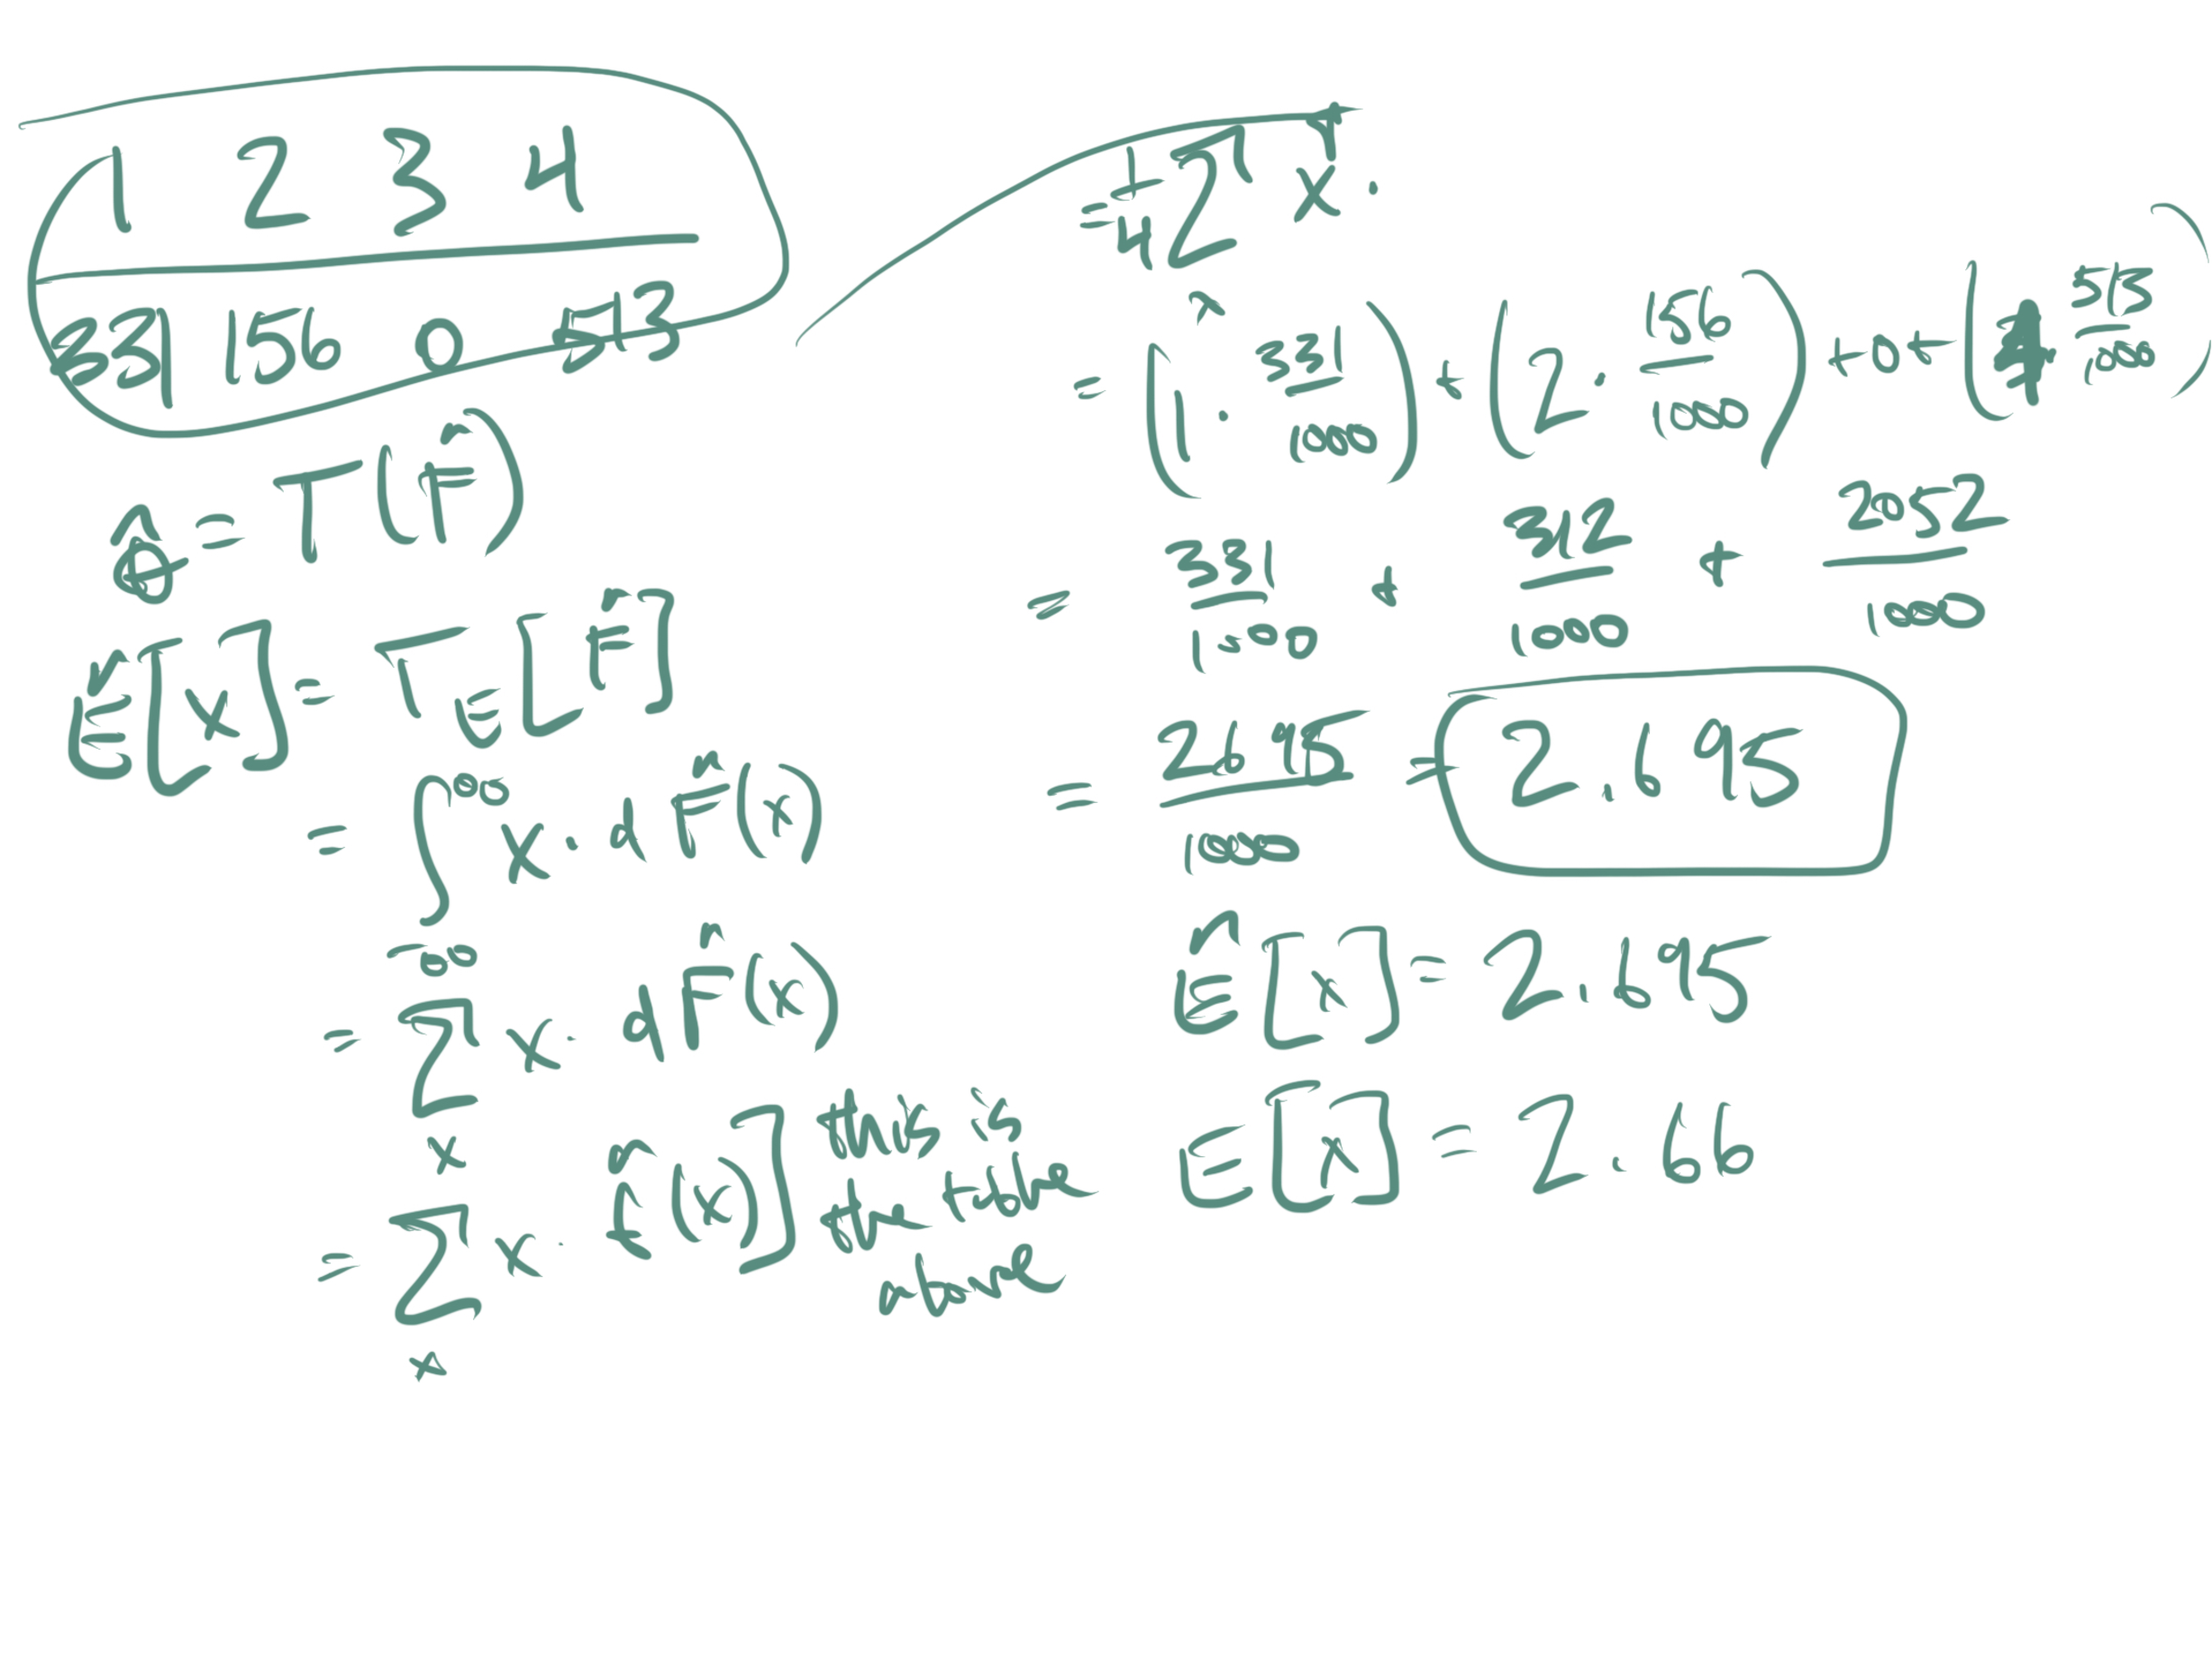
\includegraphics[width=.9\textwidth]{images/plug_in_discrete}
  }
\end{frame}

\subsection{Reading: Kernel Methods Estimate the PDF}

\begin{frame}
  \frametitle{Reading: Kernel Methods Esttimate the PDF}
  Read pages 121 - 124.   
\end{frame}
 
\subsection{Kernel Methods Estimate the PDF}

\begin{frame}
  \frametitle{Kernel Methods, Part I}
  \begin{block}{Kernel Density Estimator of PDF}
    \begin{itemize}
    \item Cannot \textit{directly} observe the joint PDF.
    \item For discrete RV, approximations come through frequency
      tables.
    \item For continuous RV, approximations come through kernel
      density estimates:
      \end{itemize} 
    \[
      \hat{f}_{K}(x) = \frac{1}{n} \sum_{i=1}^{n}K_{b}(x - X_{i}),
    \forall x \in \R\]
    
  \end{block}
\end{frame}


\begin{frame}
  \frametitle{Kernel Methods, Part II }
  \begin{itemize}
  \item Kernel methods are smoothing methods
  \item The \textit{kernel} is some weighting function
  \end{itemize}
  \begin{center}
    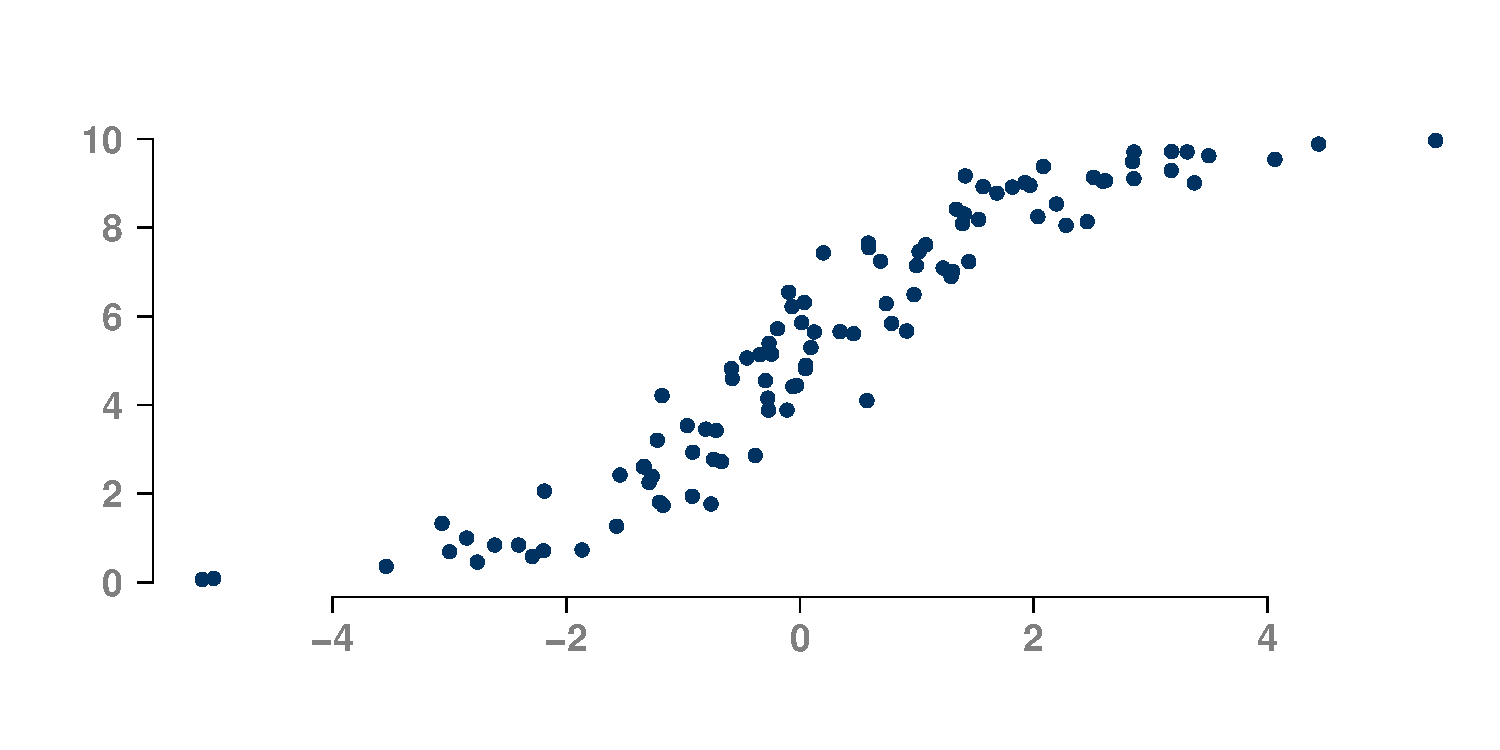
\includegraphics[width=\textwidth]{./images/logit0}
  \end{center}
  \note{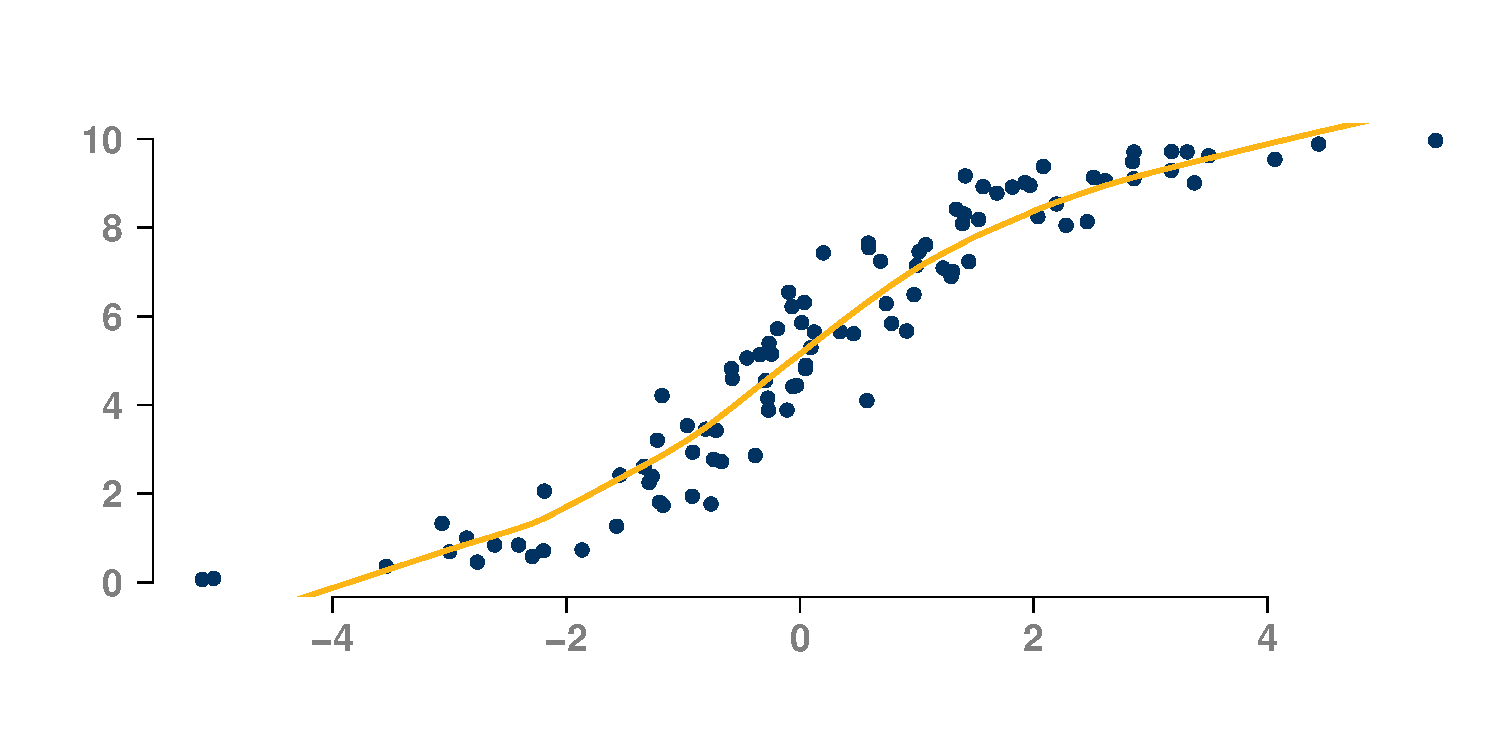
\includegraphics[width=\textwidth]{./images/logit1}}
\end{frame}


\begin{frame}
  \frametitle{Kernel Methods, part III}
  As smoothing function, these permit plug in estimates that are
  directly analogous to the estimating functionals of the CDF.
  \begin{block}{Kernel Plug-In Estimator}
    The \textit{Kernel plug-in estimator} of $\theta = T(F)$
    is \[\hat{\theta}_{k} = T\big(\hat{F}_{K}\big),\] where,
    $\hat{F}_{K} = \int_{-\infty}^{x}\hat{f}(u)du$. 
  \end{block}
  \note[item]{\paul{What's missing here is an explanation of how you get the smoothed density}}
\end{frame}

\begin{frame}
  \frametitle{Kernel Methods, part IV}
    \begin{block}{Kernel Plug-In Estimator for Expected Value}
      We know the functional for the expected value has a specific
      ``shape'' \[\E[Y] = \int y\cdot df(y).\] So, the feasible kernel method is
    \[\hat{\E}_{k}(\bs Y) = \int_{-\infty}^{\infty} y \cdot d\hat{f}_{K}(y)\]
  \end{block} 
\end{frame}

\begin{frame}[t]
  \frametitle{Kernel Methods, part V}
  \begin{itemize}
  \item $\E[Y]$ and $\E[Y|X]$ are lowest MSE estimates of $Y$
    \note[item]{But, $E[Y]$ and $E[Y|X]$ both require diety-level
      knowledge of the pdf or joint pdf.}
  \end{itemize}
  \begin{align*}
    \hat{\E}_{K}(\bs Y) &= \int y\hat{f}(y) \\ 
    \hat{\E}_{K}(\bs Y|X=x]) &= \int y \hat{f}_{Y|X}(y|x) \\
  \end{align*}
  \begin{itemize}
  \item If you can produce i.i.d. samples from $f_{Y|X}$, you can
    produce estimates, $\hat{f}_{K}(y|x)$ that get ever closer to the
    true value
  \end{itemize}
  \note[item]{The next sections in the course combine these facts with
    the CLT distributional shapes so that we can make \textbf{best}
    estimates, and we can communicate our uncertainty about these
    estimates.} 
\end{frame}



\subsection{Apply Kernel Methods}



\begin{frame}
  \frametitle{Apply Kernel Methods}
  \textbf{Note: This is a LEARNOSITY activity. We're just placing it
    here for organization.} 
\end{frame}

\end{document}
